%========================================
%                            Chapter                            
%======================================== 
\chapter{{\mv}: A Spoof-proof Voice Authentication System for Smartphones}

	Voice authentication is drawing increasing attention and becomes an attractive alternative to passwords for mobile authentication. However, existing voice authentication systems are vulnerable to various spoofing attacks. For example, attackers can record the victim's voice in person or online, then replay the recording and access the victim's devices illegally. 
We propose \shortname, a spoof-proof voice authentication system which not only differentiate different people but also differentiate live people and electronic devices. The idea is to utilize the self demodulation effect and acoustic attenuation effect when sound signals transmit through human bodies. Our system can defend the smartphone's voice authentication system against 3 attack scenarios, each contains 3 attack types. Experiments show  {\shortname} can identify different users with 94.33\% accuracy and defend voice spoofing attacks with at least 93.67\% accuracy. 
%========================================
%                            Section                             
%======================================== 	 


%\IEEEraisesectionheading{\section{Introduction}\label{sec:introduction}}
\section{Introduction}
% Computer Society journal (but not conference!) papers do something unusual
% with the very first section heading (almost always called "Introduction").
% They place it ABOVE the main text! IEEEtran.cls does not automatically do
% this for you, but you can achieve this effect with the provided
% \IEEEraisesectionheading{} command. Note the need to keep any \label that
% is to refer to the section immediately after \section in the above as
% \IEEEraisesectionheading puts \section within a raised box.




% The very first letter is a 2 line initial drop letter followed
% by the rest of the first word in caps (small caps for compsoc).
% 
% form to use if the first word consists of a single letter:
% \IEEEPARstart{A}{demo} file is ....
% 
% form to use if you need the single drop letter followed by
% normal text (unknown if ever used by the IEEE):
% \IEEEPARstart{A}{}demo file is ....
% 
% Some journals put the first two words in caps:
% \IEEEPARstart{T}{his demo} file is ....
% 
% Here we have the typical use of a "T" for an initial drop letter
% and "HIS" in caps to complete the first word.
%\IEEEPARstart{T}{his} demo file is intended to serve as a ``starter file''
%for IEEE Computer Society journal papers produced under \LaTeX\ using
%IEEEtran.cls version 1.8b and later.
%% You must have at least 2 lines in the paragraph with the drop letter
%% (should never be an issue)
%I wish you the best of success.
%
%\hfill mds
%
%\hfill August 26, 2015

%\subsection{Subsection Heading Here}
%Subsection text here.

% needed in second column of first page if using \IEEEpubid
%\IEEEpubidadjcol

%\subsubsection{Subsubsection Heading Here}
%Subsubsection text here.


% An example of a floating figure using the graphicx package.
% Note that \label must occur AFTER (or within) \caption.
% For figures, \caption should occur after the \includegraphics.
% Note that IEEEtran v1.7 and later has special internal code that
% is designed to preserve the operation of \label within \caption
% even when the captionsoff option is in effect. However, because
% of issues like this, it may be the safest practice to put all your
% \label just after \caption rather than within \caption{}.
%
% Reminder: the "draftcls" or "draftclsnofoot", not "draft", class
% option should be used if it is desired that the figures are to be
% displayed while in draft mode.
%
%\begin{figure}[!t]
%\centering
%\includegraphics[width=2.5in]{myfigure}
% where an .eps filename suffix will be assumed under latex, 
% and a .pdf suffix will be assumed for pdflatex; or what has been declared
% via \DeclareGraphicsExtensions.
%\caption{Simulation results for the network.}
%\label{fig_sim}
%\end{figure}

% Note that the IEEE typically puts floats only at the top, even when this
% results in a large percentage of a column being occupied by floats.
% However, the Computer Society has been known to put floats at the bottom.


% An example of a double column floating figure using two subfigures.
% (The subfig.sty package must be loaded for this to work.)
% The subfigure \label commands are set within each subfloat command,
% and the \label for the overall figure must come after \caption.
% \hfil is used as a separator to get equal spacing.
% Watch out that the combined width of all the subfigures on a 
% line do not exceed the text width or a line break will occur.
%
%\begin{figure*}[!t]
%\centering
%\subfloat[Case I]{\includegraphics[width=2.5in]{box}%
%\label{fig_first_case}}
%\hfil
%\subfloat[Case II]{\includegraphics[width=2.5in]{box}%
%\label{fig_second_case}}
%\caption{Simulation results for the network.}
%\label{fig_sim}
%\end{figure*}
%
% Note that often IEEE papers with subfigures do not employ subfigure
% captions (using the optional argument to \subfloat[]), but instead will
% reference/describe all of them (a), (b), etc., within the main caption.
% Be aware that for subfig.sty to generate the (a), (b), etc., subfigure
% labels, the optional argument to \subfloat must be present. If a
% subcaption is not desired, just leave its contents blank,
% e.g., \subfloat[].


% An example of a floating table. Note that, for IEEE style tables, the
% \caption command should come BEFORE the table and, given that table
% captions serve much like titles, are usually capitalized except for words
% such as a, an, and, as, at, but, by, for, in, nor, of, on, or, the, to
% and up, which are usually not capitalized unless they are the first or
% last word of the caption. Table text will default to \footnotesize as
% the IEEE normally uses this smaller font for tables.
% The \label must come after \caption as always.
%
%\begin{table}[!t]
%% increase table row spacing, adjust to taste
%\renewcommand{\arraystretch}{1.3}
% if using array.sty, it might be a good idea to tweak the value of
% \extrarowheight as needed to properly center the text within the cells
%\caption{An Example of a Table}
%\label{table_example}
%\centering
%% Some packages, such as MDW tools, offer better commands for making tables
%% than the plain LaTeX2e tabular which is used here.
%\begin{tabular}{|c||c|}
%\hline
%One & Two\\
%\hline
%Three & Four\\
%\hline
%\end{tabular}
%\end{table}


% Note that the IEEE does not put floats in the very first column
% - or typically anywhere on the first page for that matter. Also,
% in-text middle ("here") positioning is typically not used, but it
% is allowed and encouraged for Computer Society conferences (but
% not Computer Society journals). Most IEEE journals/conferences use
% top floats exclusively. 
% Note that, LaTeX2e, unlike IEEE journals/conferences, places
% footnotes above bottom floats. This can be corrected via the
% \fnbelowfloat command of the stfloats package.


\subsection{The Popularity of Voice Authentication on Smartphones}

According to reports issued by several market-research firms, the total number of smartphone users worldwide is over 3 billion this year and is expected to reach 3.9 billion by 2023~\cite{report2018newzoo,report2019forrester}. The rapid increasing use of smartphones is actuating the need for better protection. User authentication on smartphones has thus been an important area of research. 

Survey papers~\cite{vongsingthong2014survey,mahfouz2017survey,shankar2018survey} have compared the strengths and limitations of existing authentication methods, from knowledge-based methods such as PIN or password, to identity-based methods such as fingerprint and face.
%
PIN or password are the most widely used authentication methods. However, when the users have wet or dirty fingers, or wear gloves on their hands, such touchscreen-related authentication methods will not work. The fingerprint authentication suffers from the same problem. As for face recognition, it stops working when users are wearing moisturizing mask sheets or other head wearables such as ski goggles. In the aforementioned scenarios, voice authentication provides better convenience to users and thus a great alternative.


In fact, voice authentication has been adopted in a wide variety of smartphone applications. 
For example, Android users can say ``Ok Google'' to access Google assistant directly~\cite{onlinegoogle}; the Tencent company adopts Voiceprint to provide securely, faster and easier log-ins to WeChat accounts, available on both Android and iOS platforms~\cite{onlinewechat}; the BioTrust uses voice biometrics to allow elderly and sick people to order prescription medication without the need to leave the house~\cite{onlinebio}; the Citi bank uses voice biometrics authentication system for phone banking, which reduces the number of tedious security questions~\cite{onlineciti}; the LMH Blockchain adopts Say-Tec~\cite{onlinesaytec} to authenticate, validate, process, and protect users' blockchain assets and cryptocurrency by voice~\cite{onlineblockchain}.
%
Based on a market research report published in 2019~\cite{onlinemarket}, the speech and voice recognition market is expected to grow from 
 \$7.5 billion as in 2018 to  \$21.5 billion by 2024. 
 
 

\subsection{Voice Spoofing Attacks}\label{sec:spoof}
Despite of the increasing trend for the adopting of voice authentication, this method is not unassailable, just like other methods. Researchers have found that voice authentication system are vulnerable to the following four attacks~\cite{wu2015spoofing}: impersonation attack, replay attack, speech synthesis, and voice conversion.
\begin{itemize}
	\item  Impersonation attack refers to the scenario where an attacker tries to mimic the legitimate user’s voice without any computer-aided technology.
	\item Replay attack refers to the scenario where an attacker replays a pre-recorded speech sample collected from the legitimate user. 
	\item Speech synthesis refers to the scenario where an attacker generates intelligible, natural-sounding artificial speech from text.
	\item Voice conversion refers to the scenario where an attacker converts his speech signals to an artificial speech signal which has similar timbre and prosody to that of the legitimate user.
\end{itemize}


Among the four voice spoofing attacks, the impersonation attack is the hardest to perform, as Lau et al.~\cite{lau2005testing} have found that successful impersonation attacks require professional impersonators or attackers whose natural voices already similar to the legitimate user's. Even with professional mimicry artists or linguists, the existing voice authentication system is hard to fool~\cite{mariethoz2005can}.


The other three types of attacks, however, are much easier to be conducted. Because attackers could get the victim's voice recordings. It is common to see people use voice assistants (Alexa, Bixby, Cortana, Google, Siri, etc.) in public and attackers can record the victim's voice on the site or remotely. Moreover, people nowadays not only post text or image to social media sites (Facebook, Twitter, LinkedIn, YouTube, etc.), but also upload videos containing their voices. Attackers can extract the victim's voice from those online videos and build the speech profile of each victim. With a properly built speech profile, attackers are able to use the victim's voice to say just about anything, using algorithms such as vector quantization~\cite{abe1990voice}, probabilistic transform~\cite{stylianou1998continuous}, or neural networks~\cite{desai2009voice}. Such voice generation techniques are well-established. As an evidence, celebrity voice changer websites or apps could generate natural sounding speeches as from Obama, Trump, Stephen Hawking, Bruce Wayne, and many more.




Some may argue that large training data is required to build the victim's speech profile. However, for the purpose of attacking, the attackers may only need to use small training data to generate the hotword or the activation phrase. There is no need to generate every possible sentence. This is because most voice authentication systems adopts a one-time authentication scheme to grant access, instead of a continuous authentication scheme~\cite{feng2017continuous}.

\begin{landscape}
	\begin{figure*}[h]
		\begin{minipage}[t]{0.33\textwidth}
			\fbox{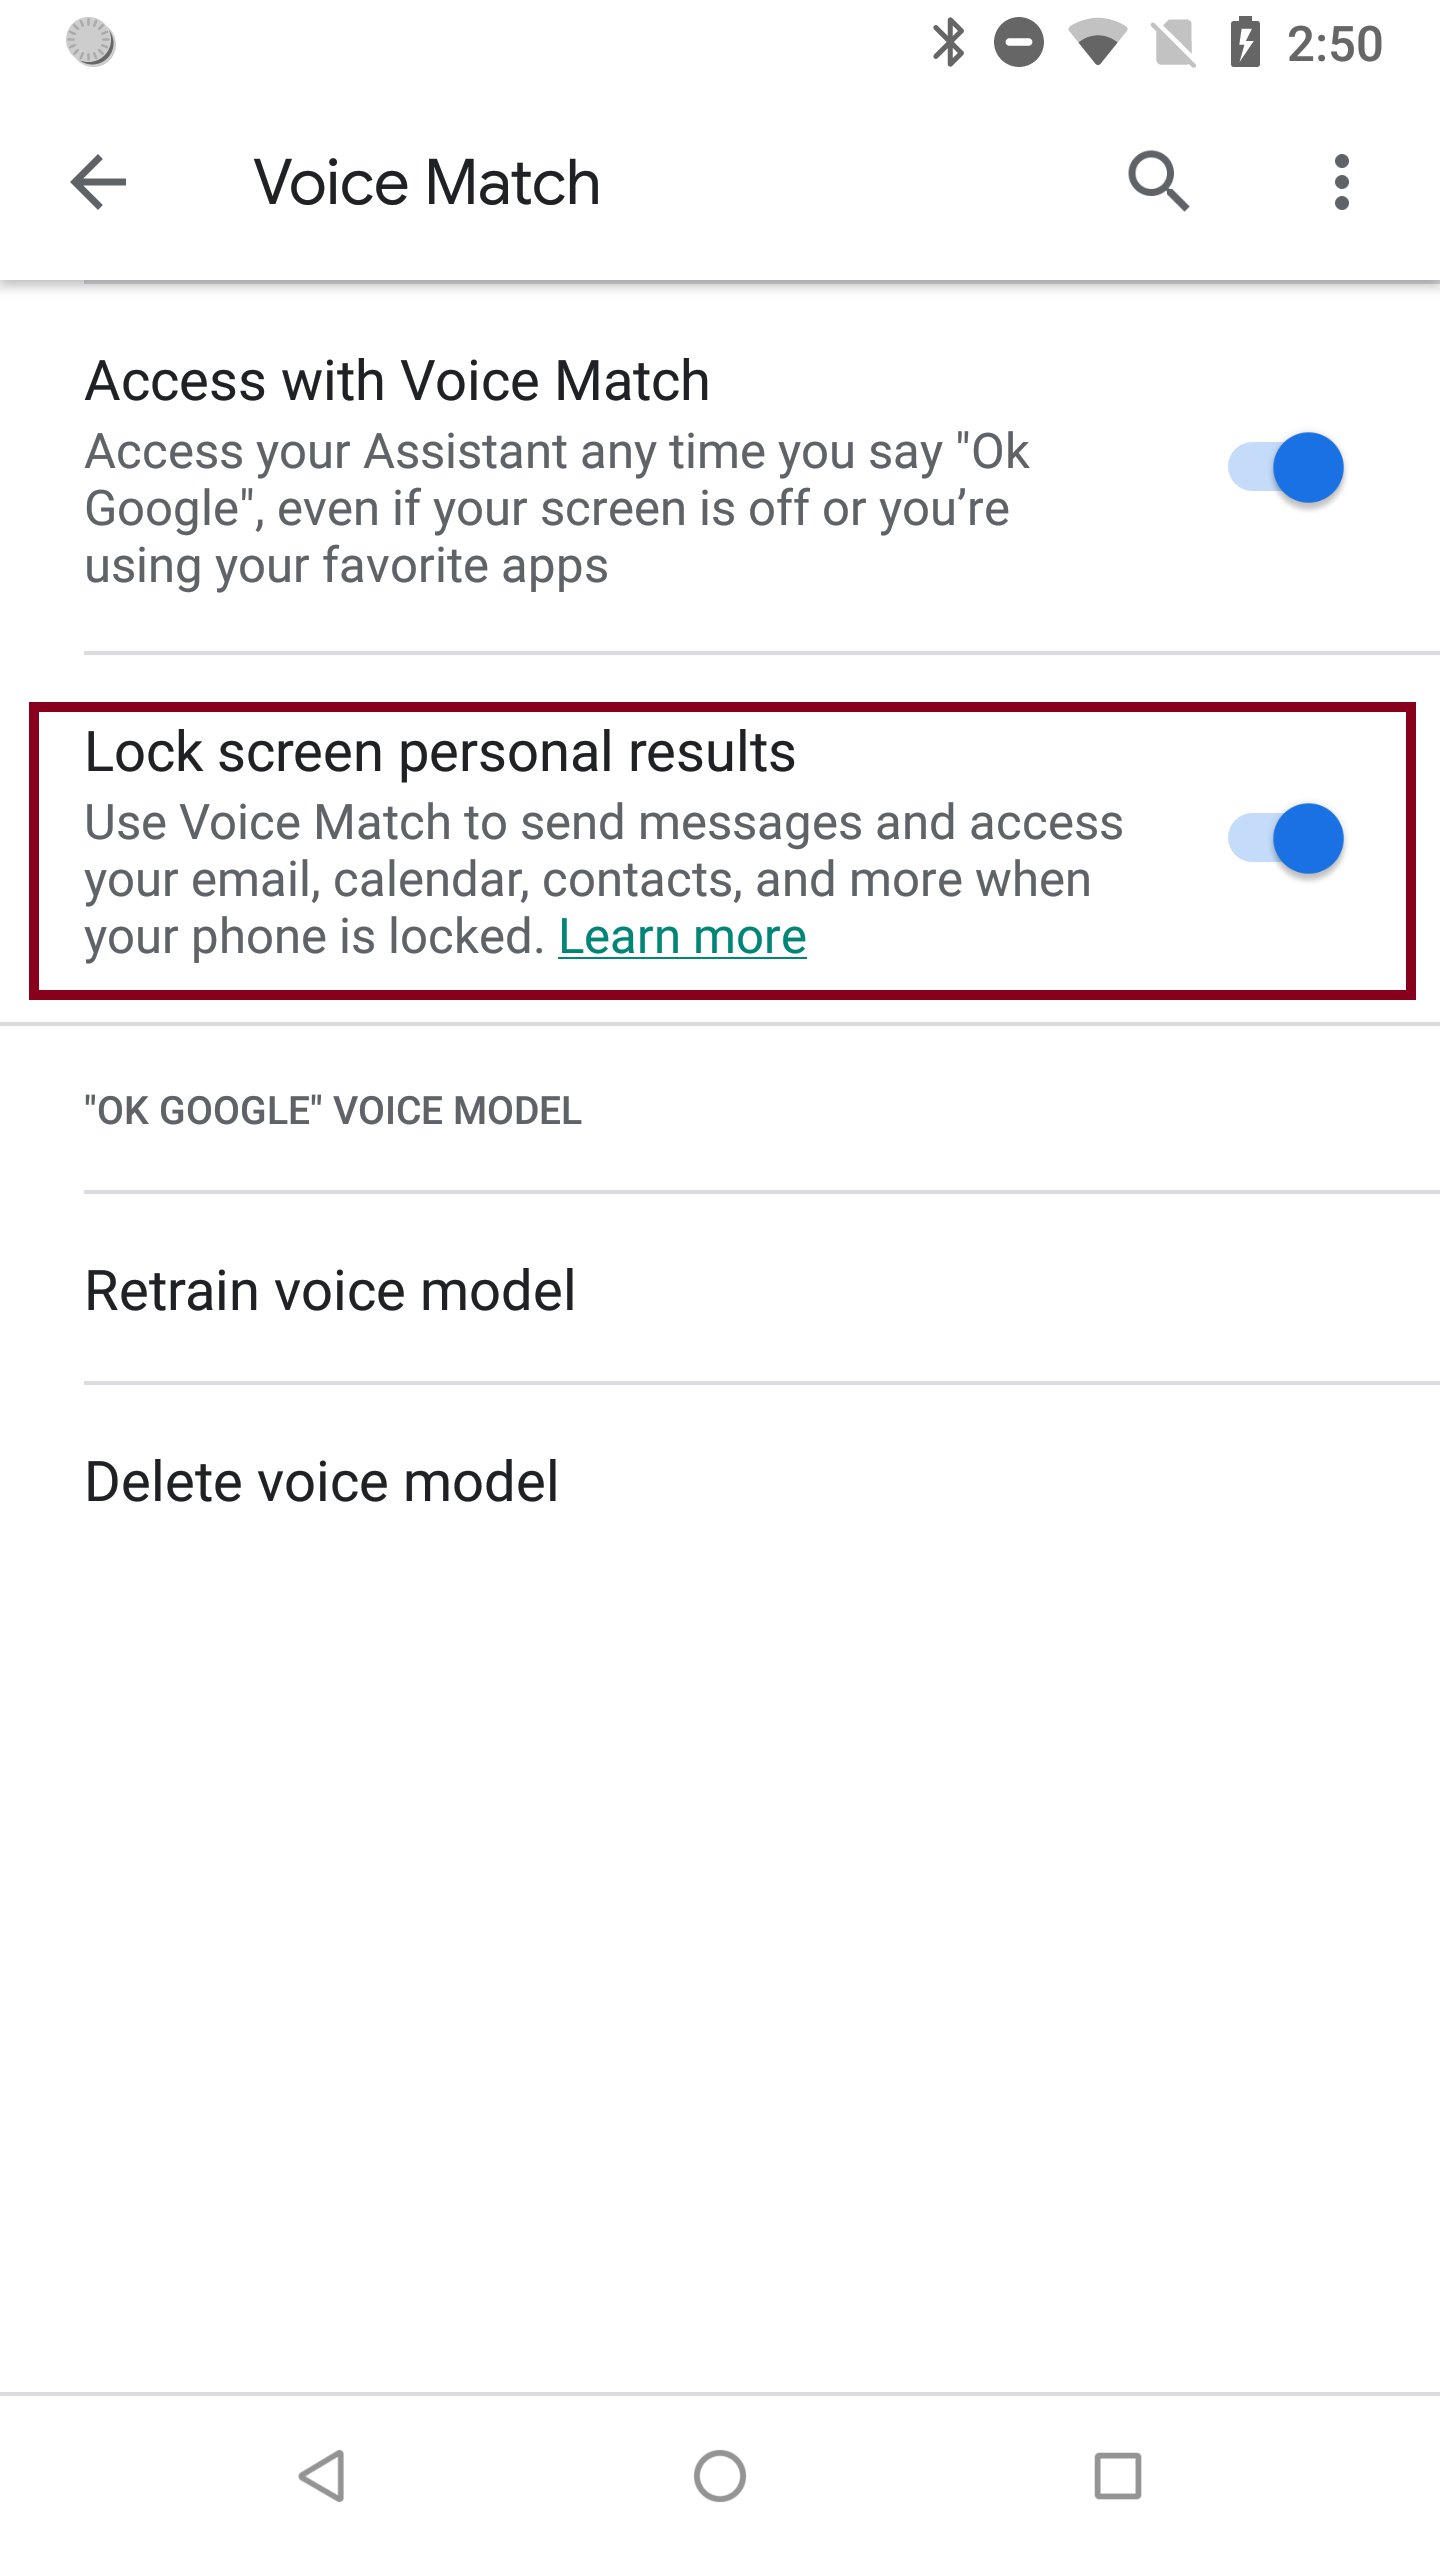
\includegraphics[width=1.2\textwidth]{voicematch}}
			\subcaption{Enabling Voice setting.}
			\label{fig:voicematch}
		\end{minipage}
		\hspace{1in}
		\begin{minipage}[t]{0.33\textwidth}
			\fbox{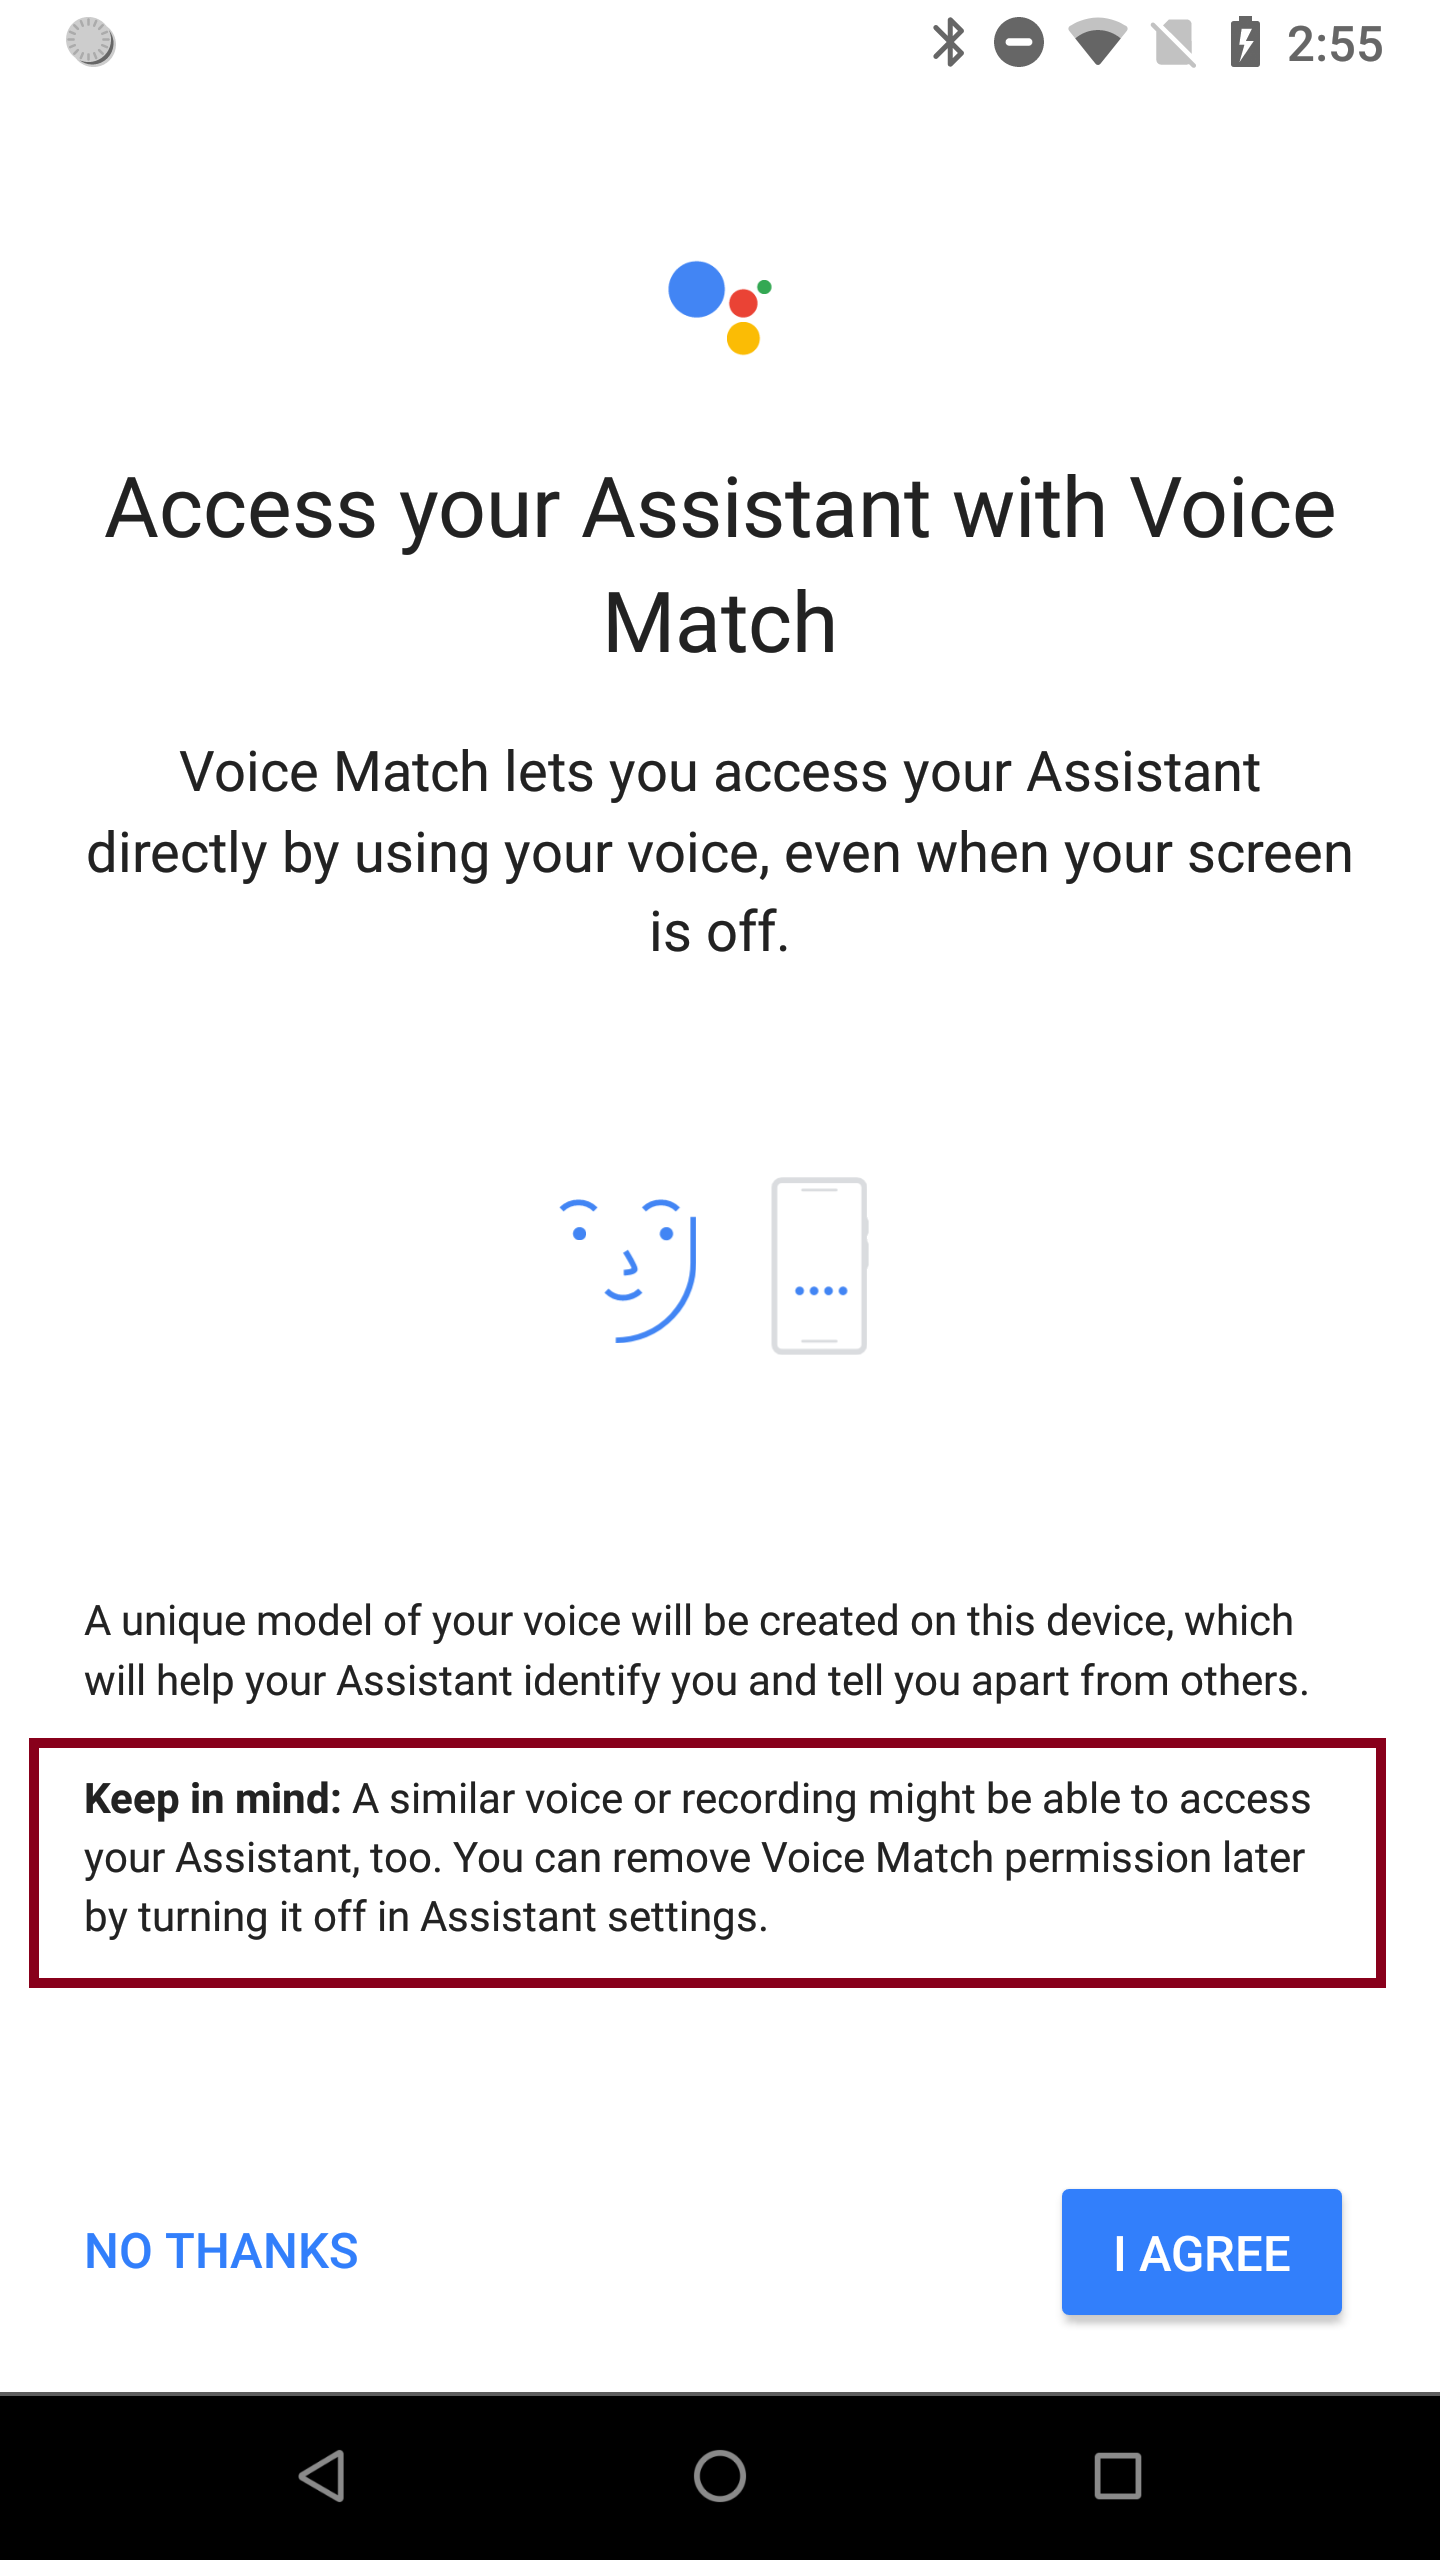
\includegraphics[width=1.2\textwidth]{voicematch2}}
			\subcaption{Voice Match warning.}
			\label{fig:voicematch2}
		\end{minipage}
		\hspace{1in}
		\begin{minipage}[t]{0.33\textwidth}
			\fbox{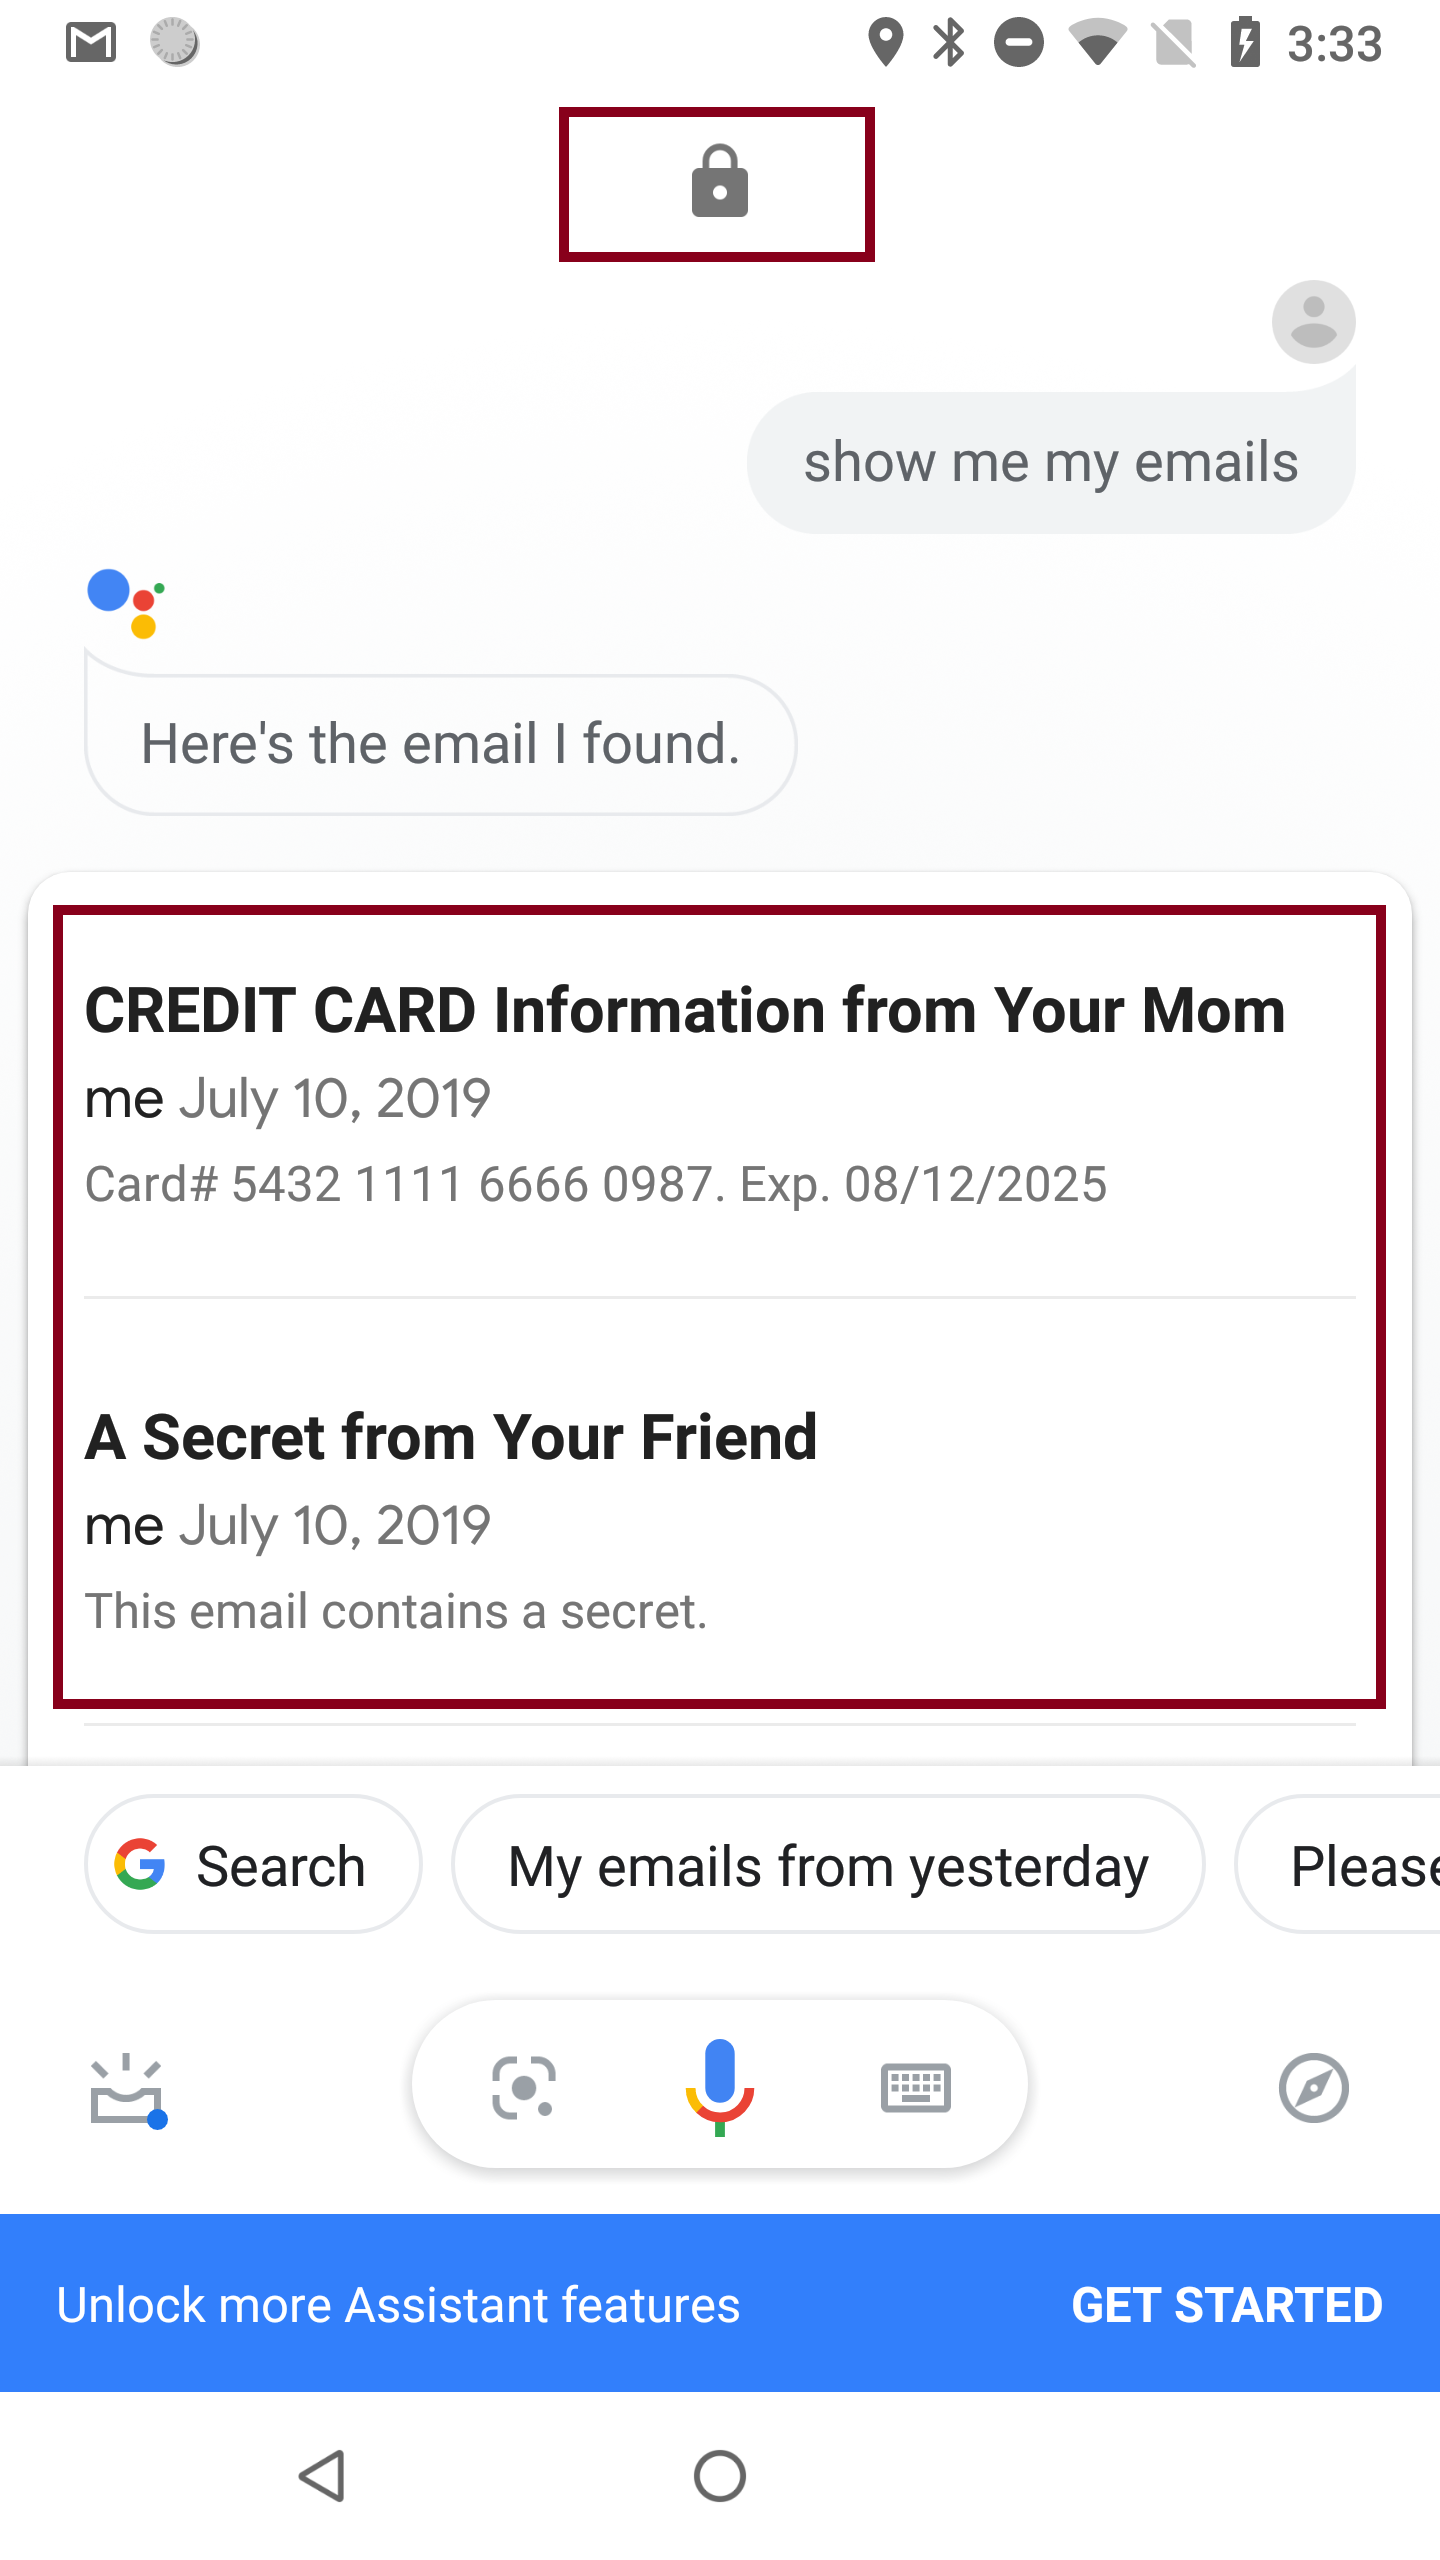
\includegraphics[width=1.2\textwidth]{email}}
			\subcaption{Information leakage when the phone is locked. }
			\label{fig:email}
		\end{minipage}  
	\vspace{-.05in}
		\caption{Screenshots about Voice Match on Google Nexus 6P.}\label{fig:example}
	\end{figure*}
\end{landscape}

For example, on a Google Nexus~6P smartphone running Android 8.1.0, it provides the Voice Match feature which allow users to access their personal data by voices\footnote{When the Voice Match feature first came out, Android users could fully unlock the phone with this function. However, starts from January 2019, Google removes the ability for Voice Match to act as a password due to security concerns. The previous ``Unlock with Voice Match'' is replaced to only providing ``personal results''. Such results come from emails, calendar entries, contacts, etc., and are still sensitive information.}. If an attacker replays the victim's ``Ok Google'' utterance, followed by ``show me my emails'' in his own voice (not the victim's), the Android system will regard him as the legitimate user (false acceptance) and show the emails. Because the authentication only check the hotword. Once the access is granted, any command coming after will be executed, no matter in whose voice.


Fig.~\ref{fig:example} are the screenshots when the aforementioned replay attack is tested in reality. Fig.~\ref{fig:voicematch} shows how to enable the Voice Match function. Fig.~\ref{fig:voicematch2} indicates the system is aware of its vulnerability to impersonation attack and replay attack. Fig.~\ref{fig:email} demonstrates the attacker could steal sensitive information without unlocking the phone (the closed padlock at the top). In this test, the leaked information are emails from the Gmail Inbox, which include the credit card information sent from the victim's mom and a secret from his friend. Recall that to conduct this attack successfully, all the thing the attacker need is a short recording of ``Ok Google'' in the victim's voice, but the harm can be huge.


\subsection{Liveness Detection}
Voice spoofing attacks drastically degrade the performance of standard voice authentication systems by increasing false acceptance rates~\cite{wang2011channel, ergunay2015vulnerability}, leading to severe security and privacy issues. Fortunately, researchers have done extensive research on defending these attacks and building spoof-proof voice authentication systems.




\begin{landscape}
	\SingleSpacing
	
	\begin{longtable}{p{3cm}p{6cm}p{6cm}ccc} %p{1.5cm}
		\caption{Related Work on Liveness Detection}
		\label{tab:liveness}
		\\
		
		\toprule
				Authors & Method & Shortcomming & Accuracy & \shortstack{No Extra \\ Devices} &  \shortstack{No Cumbersome \\ User Interaction}  \\
	%			& No User-specific Training\\
		\midrule
		
		\endfirsthead
		
		\normalfont\tablename~\thetable{}~Continued\\
		\toprule
				Authors & Method & Shortcomming & Accuracy & \shortstack{No Extra \\ Devices} &  \shortstack{No Cumbersome \\ User Interaction}  \\
	%			& No User-specific Training\\
		\midrule
		
		\endhead
		
		\bottomrule		
		\endfoot
		
		\endlastfoot
			Girija Chetty and Michael Wagner~\cite{chetty2004automated} & Detecting lip movements using cameras. & Inherits shortcomings of face authentication and introduces high computational overhead. & 99\% & \xmark & \cmark \\
%			& \xmark\\
			Poss et al.~\cite{poss2008biometric} & Using neural tree networks to determine unique aspects of utterances and Hidden Markov Models to classify them. & The accuracy is unkown. & - & \cmark & \cmark 
			\\
%			& \xmark \\
			Wei Shang and Maryhelen Stevenson~\cite{shang2010score} & Testing whether an incoming recording shares the same originating utterance as any of N stored recordings. & Performance is largely based on the pre-stored recordings. & 88.1\%/93.2\% & \cmark & \cmark 
			\\
%			& \xmark \\
			Jes{\'u}s Villalba and Eduardo Lleida~\cite{villalba2011detecting} & Detecting noises and spectrum changes caused by far-field microphone and loudspeakers. & Limits the replay attackers to use far-field microphones. & 91\%-100\% & \cmark & \cmark \\
%			& \cmark \\
			Wang et al.~\cite{wang2011channel} & Detecting channel pattern noise caused by microphone and loudspeakers. & Limits the replay attackers to use low-quality microphones. & 97\% & \cmark & \cmark 
			\\
%			& \cmark \\			
			Aley-Raz et al.~\cite{aley2013device}  & Integrating intra-session voice variation to Nuance VocalPassword~\cite{onlinenuance}. & Requires the user to cumbersomely repeat prompted sentences. & - & \cmark & \xmark 
			\\
%			& \cmark \\
			Zhang et al.~\cite{zhang2016voicelive} & \textbf{VoiceLive}: Measuring the time-difference-of-arrival changes of a sequence of phoneme sounds to the two microphones of the phone. & Requires at least two high-quality microphones in one smartphone. & 99\% & \cmark & \cmark 
			\\
%			& \xmark \\
			Chen et al.~\cite{chen2017you} & Detecting the magnetic field emitted from loudspeakers. & Requires the user to move the smartphone with the predefined trajectory around the sound source. & 100\% & \cmark & \xmark 
			\\
%			& \cmark \\			
			Zhang et al. ~\cite{zhang2017hearing} & \textbf{VoiceGesture}: Leverages Dopler shifts in signals caused by users' articulatory gestures when speaking. & Requires high quality microphones and needs a longer computation time. & 99\% & \cmark & \cmark
			\\
%			 & \xmark \\
			Feng et al.~\cite{feng2017continuous}  & \textbf{VAuth}: Utilizing the instantaneous consistency of the entire signal from the accelerometer and the microphone. & Requires the user to wear high-sampling-rate accelerometers on the facial, throat, or sternum areas. & 97\% & \xmark & \cmark 
			\\
%			& \cmark \\
			Huang et al.~\cite{huang2018breathlive}  & \textbf{BreathLive}: Utilizing chest movement when making deep breaths & The sound is deep breath sound instead of human speech; Stethoscope is needed. & 91\%/94\%/96\% & \xmark & \cmark 
			\\
%			& \xmark \\
			Ment et al.~\cite{meng2018wivo} & \textbf{WiVo}: Using channal state information (CSI) from WiFi signals to detect mouth movement  &  Requires WiFi antennas to collect the CSI info; the distance between antennas and human is short (20cm). & 99\% & \xmark & \cmark
 \\
\bottomrule

\end{longtable}

\end{landscape}

%\begin{landscape}	
%	\begin{table}
%		\centering
%%		\renewcommand{\arraystretch}{1.5}
%%		\caption{Related Work on Liveness Detection}
%%		\label{tab:liveness}
%		\footnotesize
%		\begin{tabular}{p{2.5cm}p{0.5cm}p{4.5cm}p{4.5cm}ccc} %p{1.5cm}
%			\toprule\specialrule{0.5pt}{1.5pt}{\belowrulesep}
%			Authors & Year & Method & Shortcomming & Accuracy & \shortstack{No Extra \\ Devices} &  \shortstack{No Cumbersome \\ User Interaction}  \\
%%			& No User-specific Training\\
%			\midrule
%			Girija Chetty and Michael Wagner~\cite{chetty2004automated} & 2004 & Detecting lip movements using cameras. & Inherits shortcomings of face authentication and introduces high computational overhead. & 99\% & \xmark & \cmark \\
%%			& \xmark\\
%			Poss et al.~\cite{poss2008biometric} & 2008 & Using neural tree networks to determine unique aspects of utterances and Hidden Markov Models to classify them. & The accuracy is unkown. & - & \cmark & \cmark 
%			\\
%%			& \xmark \\
%			Wei Shang and Maryhelen Stevenson~\cite{shang2010score} & 2010 & Testing whether an incoming recording shares the same originating utterance as any of N stored recordings. & Performance is largely based on the pre-stored recordings. & 88.1\%/93.2\% & \cmark & \cmark 
%			\\
%%			& \xmark \\
%			Jes{\'u}s Villalba and Eduardo Lleida~\cite{villalba2011detecting} & 2011 & Detecting noises and spectrum changes caused by far-field microphone and loudspeakers. & Limits the replay attackers to use far-field microphones. & 91\%-100\% & \cmark & \cmark \\
%%			& \cmark \\
%			Wang et al.~\cite{wang2011channel} & 2011 & Detecting channel pattern noise caused by microphone and loudspeakers. & Limits the replay attackers to use low-quality microphones. & 97\% & \cmark & \cmark 
%			\\
%%			& \cmark \\			
%			Aley-Raz et al.~\cite{aley2013device}  & 2013 & Integrating intra-session voice variation to Nuance VocalPassword~\cite{onlinenuance}. & Requires the user to cumbersomely repeat prompted sentences. & - & \cmark & \xmark 
%			\\
%%			& \cmark \\
%			Zhang et al.~\cite{zhang2016voicelive} & 2016 & \textbf{VoiceLive}: Measuring the time-difference-of-arrival changes of a sequence of phoneme sounds to the two microphones of the phone. & Requires at least two high-quality microphones in one smartphone. & 99\% & \cmark & \cmark 
%			\\
%%			& \xmark \\
%			Chen et al.~\cite{chen2017you} & 2017 & Detecting the magnetic field emitted from loudspeakers. & Requires the user to move the smartphone with the predefined trajectory around the sound source. & 100\% & \cmark & \xmark 
%			\\
%%			& \cmark \\			
%			Zhang et al.~\cite{zhang2017hearing} & 2017 & \textbf{VoiceGesture}: Leverages Dopler shifts in signals caused by users' articulatory gestures when speaking. & Requires high quality microphones and needs a longer computation time. & 99\% & \cmark & \cmark
%			\\
%%			 & \xmark \\
%			Feng et al.~\cite{feng2017continuous}  & 2017 & \textbf{VAuth}: Utilizing the instantaneous consistency of the entire signal from the accelerometer and the microphone. & Requires the user to wear high-sampling-rate accelerometers on the facial, throat, or sternum areas. & 97\% & \xmark & \cmark 
%			\\
%%			& \cmark \\
%			Huang et al.~\cite{huang2018breathlive}  & 2018 & \textbf{BreathLive}: Utilizing chest movement when making deep breaths & The sound is deep breath sound instead of human speech; Stethoscope is needed. & 91\%/94\%/96\% & \xmark & \cmark 
%			\\
%%			& \xmark \\
%			Ment et al.~\cite{meng2018wivo} & 2018 & \textbf{WiVo}: Using channal state information (CSI) from WiFi signals to detect mouth movement  &  Requires WiFi antennas to collect the CSI info; the distance between antennas and human is short (20cm). & 99\% & \xmark & \cmark
%			\\
%		\specialrule{0.5pt}{\aboverulesep}{1.5pt}\bottomrule
%		\end{tabular}
%	\end{table}
%\end{landscape}

%Shang et al.~\cite{shang2010score} propose to compare an input voice sample with stored instances of past accesses to detect the voice samples have been seen before by the authentication system. This method, however, cannot work if the attacker records the voice samples during a non-authentication time point. Villalba et al. and Wang et al. suggest that the additional channel noises introduced by the recording and loudspeaker can be used for attack detection~\cite{villalba2011detecting,wang2011channel}.
%These approaches however have limited effec- tiveness in practice. For example, the false acceptance rates of these approaches are as high as 17\%. Chetty and Wagner propose to use video camera to extract lip movements for liveness verification~\cite{chetty2004automated}, whereas Poss et al. combine the techniques of a neural tree network and Hidden Markov Models to improve authentication accuracy~\cite{poss2008biometric}.
%Aley-Raz et al.~\cite{aley2013device} develop a liveness detection system based on ``Intra-session voice variation'', which is integrated into Nuance VocalPassword~\cite{onlinenuance}. In addition to a user-chosen passphrase, it requires a user to repeat one or more random sentences prompted by the system for liveness detection. Such a method however increases the op- eration overhead of the user and is cumbersome due to an explicit user cooperation is required besides the standard authentication process. 
%
%More recently, Chen et al.~\cite{chen2017you} develop a smartphone based liveness detection system by measuring the magnetic field emit- ted from loudspeakers. It however requires the user to speak the passphrase while moving the smartphone with predefined trajectory around the sound source. Moreover, Zhang et al.~\cite{zhang2016voicelive} propose a smarthphone based solution, which measures the time-difference-of-arrival (TDoA) changes of a sequence of phoneme sounds to the two microphones of the phone when a user speaks a passphrase for liveness detection. However, it requires at least two high-accuracy microphones in one smartphone. Zhang et al.~\cite{zhang2017hearing} then propose VoiceGuesture, which leverages a user’s articulatory gestures when speaking a passphrase for liveness detection. However, the calculation overhead is high.
%Feng et al.~\cite{feng2017continuous} present VAuth,  which utilizes the instantaneous consistency of the entire signal from the accelerometer and the microphone.  However, it requires the user to wear a security-assisting device on the facial, throat, or sternum areas. 
%Huang et al.~\cite{huang2018breathlive} present BreathLive, which utilize the inherent correlation between sounds and chest motion caused by deep breathing to realize a reliable liveness detection system. However, it requires special gyroscope and stethoscope. Since it utilizes deep breathing, the sound period is very long (4 sec. for one deep breathing).
%
%In conclusion, the aforementioned approaches either require cumbersome user interaction, or require extra electronic devices, or require long recording time or processing time. Building a good liveness detection component is still an open problem.

As mentioned in Section~\ref{sec:spoof}, the threat of impersonation attack is much less than that of the other three attacks, so impersonation attack is not a research focus. For replay attack, speech synthesis, and voice conversion, researchers have noticed that they have one thing in common -- the attacking sound is played by an electronic speaker\footnote{In this and many other papers, attackers must play the attacking sound near the targeted smartphone. We do not consider the scenario where sound files are directly injected. Because if attackers can inject sounds to the system, the phone is already hacked. So there is no need to go through the voice authentication procedure anymore.} rather than spoken by a real person. Therefore, if the authentication system can distinguish whether the sound comes from a live person or an electronic device, it would be immune from those voice spoofing attacks.



Existing liveness detection methods can be classified into two groups: detecting human-related characteristics, or detecting device-related characteristics. 

As listed in Table~\ref{tab:liveness}, there have been many researches on detecting human-related characteristics.  
Girija Chetty and Michael Wagner~\cite{chetty2004automated} use cameras to detect lip movements to detect liveness. However, their work requires the camera access and inherits the shortcomings of face authentication systems. Similarly, Meng et al.~\cite{meng2018wivo} tries to detect mouth movement, but from channel state information from WiFi signals. Their approach requires antenna pairs and the antennas are placed very close to human (20cm), which is not practical in reality.
Poss et al.~\cite{poss2008biometric} use neural tree networks to determine unique aspects of utterances and hidden Markov models to classify those features. However, their work requires high computing power and long processing time. 
Wei Shang and Maryhelen Stevenson~\cite{shang2010score} detect liveness by testing whether an incoming recording shares the same originating utterance as any of previously-stored recordings. However, the performance of their work is largely based on the previously-stored recordings. 
Aley-Raz et al.~\cite{aley2013device} integrate intra-session voice variation to Nuance VocalPassword~\cite{onlinenuance} for liveness detection, but they require the user to cumbersomely repeat prompted sentences.
Zhang et al.~\cite{zhang2016voicelive} detect liveness by measuring the time-difference-of-arrival changes of a sequence of phoneme sounds using the two microphones of the phone, which requires at least two high-quality microphones in one smartphone. They also propose another work~\cite{zhang2017hearing} to detect users' articulatory gestures when speaking. However, their work requires high quality microphones again and needs a longer computation time.
Last but not least, Feng et al.~\cite{feng2017continuous}  utilizes the instantaneous consistency of the entire signal from the accelerometer and the microphone for liveness detection. Their work is the most closely related work to ours. However,  their work requires the user to wear extra accelerometers on the facial, throat, or sternum areas. Moreover, the accelerometer used in their work requires a very high sampling rate (11,000 Hz), which cannot be supported by current smartphones. In this work, we are only using a 400 Hz sampling rate for the accelerometer and the gyroscope.

The aforementioned researchers detects the liveness of a user directly, but we can also detect the liveness from the reverse side: detecting the presence of electronic devices. For example, Jes{\'u}s Villalba and Eduardo Lleida~\cite{villalba2011detecting}  detect noises and spectrum changes caused by far-field microphone and loudspeakers. Wang et al.~\cite{wang2011channel} detect channel pattern noise caused by microphone and loudspeakers to identify replay attackers. However, they can only deal with attackers who use low-quality microphones to record the legitimate user's voices or record the voice at a long distance. More recently, Chen et al.~\cite{chen2017you} detects the magnetic field emitted from loudspeakers to identify attacks, but their work requires the user to move the smartphone with the predefined trajectory around the sound source.


In conclusion, liveness detection methods either detect the presence of human beings or the presence of electronic devices. Existing work has at least one of the following shortcomings: 1) requiring special or extra devices; 2) requiring cumbersome user interaction; 3) requiring high computing power or long processing time; 4) limited ability in defending against spoofing attacks. Therefore, building a spoof-proof voice authentication system is still an open problem.



%TODO computation power
%less energy
%sensitive to surrounding noise



\begin{figure}[!h]
	\centering
	\begin{subfigure}[t]{0.15\textwidth}
		\centering
		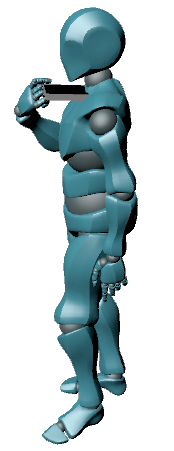
\includegraphics[height=1.8in]{standing}
		\caption{Standing}
	\end{subfigure}%
	~ 
	\begin{subfigure}[t]{0.15\textwidth}
		\centering
		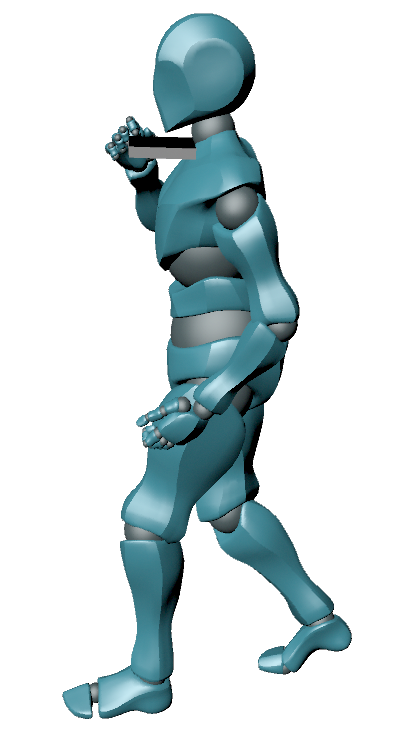
\includegraphics[height=1.8in]{walking}
		\caption{Walking}
	\end{subfigure}
	~ 
	\begin{subfigure}[t]{0.15\textwidth}
		\centering
		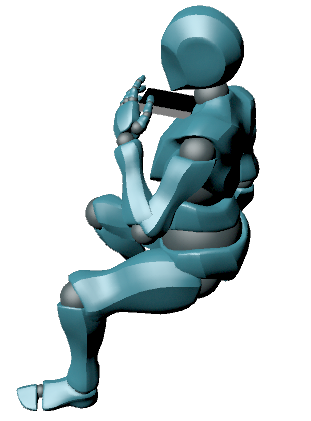
\includegraphics[height=1.8in]{sitting}
		\caption{Sitting}
	\end{subfigure}
	\caption{Authentication scenario of {\shortname}: holding the smartphone in contact with the throat while authenticating. In this way, the smartphone captures the body-borne voice vibrations through accelerometers and gyroscopes.}
	\label{fig:use}
\end{figure}

%TODO Add position test

\subsection{Overview of {\shortname}}

In this thesis, we propose {\shortname}, a spoof-proof voice authentication system that using \underline{mo}tion sensors (accelerometers and gyroscopes) to measure \underline{vo}ice.


As shown in Fig.~\ref{fig:use}, the user places the smartphone horizontally and makes sure the phone is in close contact with his throat. Then the embedded motion sensors inside the phone captures the conductive vibrations from vocal organs to the throat, and to the smartphone. Afterwards, the collected motion sensor data will be used for user authentication.


The intuition behind {\shortname} is the fact that human voice is essentially vibrations, so it can be recorded by motion sensors ~\cite{hopkin2003getting,o2009sonic,michalevsky2014gyrophone}.  Such motion-sensor data can be regarded as downsampled microphone data, so it has potentials to be used for voice authentication too. 
%
Moreover, since human body is a nonlinear medium similar to water~\cite{kim2014sound}, sounds go through the body will be affected by acoustic attenuation~\cite{szabo1994time} and self demodulation~\cite{berktay1965possible}. Such effects are human-only effects in that electronic devices are not water-like medium and have totally different acoustic properties. Therefore, using motion data for authentication can effectively differentiate live people from electronic devices, so that the system is protected against various voice spoofing attacks.

In fact,  there have been some recent studies that show the possibility of acquiring acoustic signals by smartphones' motion sensors. Michalevsky et al.~\cite{michalevsky2014gyrophone} proposed \textit{Gyrophone} in 2014. To the best of our knowledge, they are the first to use smartphone gyroscopes as low-frequency microphones to listen to loudspeakers. Gyrophone can differentiate 11 digits\footnote{One, two, \ldots, nine and zero.} with 65\% accuracy based on a 10 people dataset.
%
One year later, Zhang et al.~\cite{zhang2015accelword} proposed \textit{AccelWord}, which utilizes accelerometers to classify hotwords such as ``Okay Google'' or ``Hi Galaxy'' over other short phrases with 85\% accuracy. AccelWord is also tested over 10 people.
%
In 2018, however, Anald and Saxena~\cite{anand2018speechless} reproduced the aforementioned works and overturned their conclusions. They argued that smartphone motion sensors can not be affected by the speech signals transmitted through the air, no matter the sound source is a loudspeaker or a live person. They reported that only when the speakers and the motion sensors sharing a surface,  the  conductive vibrations will affect motion sensors' readings. Consisting with this newest research, {\shortname} asks the user to press the phone on his throat so that the body-borne vibrations are recorded, not the air-borne sounds.

%Except for this ``Loudspeaker-Same-Surface'' scenario, they studied 5 other  scenarios\footnote{``Loudspeaker-Different-Surface'',
%	``Laptop-Same-Surface'', `` Phone-Different-Surface'', 		``Human-Normal'',
%	and ``Human-Loud''.} and concluded that smartphone motion sensors only pose a limited threat to speech privacy.
% since conductive vibrations are ``possibly less common''.
%the impact of speech signals is very limited on motion sensors. 

%However, they missed one important scenario,  the \textit{intra-device} scenario, where the speakers and motion sensors are inside the same smartphone. The side-channel attack in this scenario, or the \textit{{\attackName}} attack as we refer to it, is the focus of this paper. We agree with Anald and Saxena on that motion sensors are more sensitive to conductive vibrations than aerial vibrations, but we show motion sensors can leak various critical information and pose a big threat to smartphone users' security and privacy. 


In summary, compared to previous works, the {\shortname} system have the following features:
\begin{itemize}
	\item  \textbf{All-in-One}: {\shortname} is an integral method which handles user authentication and liveness detection at the same time.
	
	\item  \textbf{Applicable}: {\shortname} works with current-off-the-shelf commercial smartphones. It does not require any extra electronic device nor any special phone model, since the sensors being used (motion sensors) are embedded on almost every smartphones.
	
	\item \textbf{Easy}: Except for pressing the smartphone on the user’s throat, {\shortname} does not ask users to do extra movements other than an ordinary speaking behavior.  
	
	\item \textbf{Improved Robust}: General voice authentication systems are sensitive to the surrounding noises and their performance will degrade a lot in noisy environments. {\shortname}, however, will not be affected. This is because smartphone's motion sensors measure the conductive vibrations and the  affection from air-borne sounds is very limited~\cite{anand2018speechless}.

%TODO change algorithms
%	\item \textbf{Computational Efficient}: {\shortname} has low computational overhead. For the same speech, motion data has a much smaller size  than that of microphones, because of the lower sampling rate (as shown in Table~\ref{tab:sample}). 
%%	Therefore, processing motion data is faster.
%	
%	\item \textbf{Energy Saving}: Motion sensors consume less energy than microphones ~\cite{zhang2015accelword}. 
	
	%TODO  section name
	\item \textbf{Expandable}: MoVo currently is a  text-dependent voice authentication systems that detects certain hotwords. However, it can be expanded to a text-independent system since it is syllable-based (will be elaborated in Section~\ref{sec:system}).
	
	
	%TODO accuracy	
%	\item
\end{itemize}




% and are dependent on the unique body structures of different people. Therefore, the data collected by motion sensors can be used for authentication and is spoof-proof.

%using the motion sensor measured voice to do authentication, instead of the microphone data, can effectively protect the system from voice spoofing attacks.



%
%As shown in Fig.~\ref{fig:use}, \shortname~records the user's voices by built-in microphones and the user's throat movement by the motion sensors at the same time. Only when these two types of signals match each other, the user is considered as a live person; otherwise, the user is rejected immediately.
%
%%\begin{figure}[!h]
%%	\centering
%%	\begin{tikzpicture}
%%	\draw (0, 1) node[inner sep=0] {\includegraphics[width=.2\linewidth]{use}};
%%	\draw (3, 1.5) node {\footnotesize\textsf{\qquad Speech -> Microphones} };
%%	\draw (4, 0) node {\footnotesize\textsf{\qquad throat Movement -> Accelerometers and Gyroscopes} };
%%	\end{tikzpicture}
%%	\caption{Authentication scenario of \shortname: placing the smartphone on the throat when speaking. In this way, the smartphone captures the audio signals by microphones and throat movements by motion sensors simultaneously.}
%%	\label{fig:use}
%%\end{figure}
%
%Although it is easy to be accepted that a person's voice and his throat movement are closely correlated,  the corresponding speech signals and motion data are not easy to be matched. The challenges are:
%\begin{itemize}
%	\item The gap between the sampling frequencies of different sensors is large. The microphone sensor on commercial off-the-shelf smartphones has a typically 44.1 kHz or 48 kHz sampling frequency~\cite{onlinemicrophone}, while the accelerometer and gyroscope has a typical 200 Hz maximum sampling frequency~\cite{michalevsky2014gyrophone}. Note that the inherent sampling frequency of MEMES sensors on smartphones is actually higher than the above values~\cite{suprem2017orientation}. However, the operating system restricts the rate.
%	\item The on-body vibration created by the sound production is subtle. Moreover, since the motion sensors are embedded in smartphones, they are not directly contacted, which further lowers the readings.
%	\item The noises caused by other body movements, heart beats, and breathings are strong interference. 
%\end{itemize}
%
%%TODO proof-of-concept
%
%%TODO figures about challenges
%\begin{figure}[h]
%%	\centering
%%	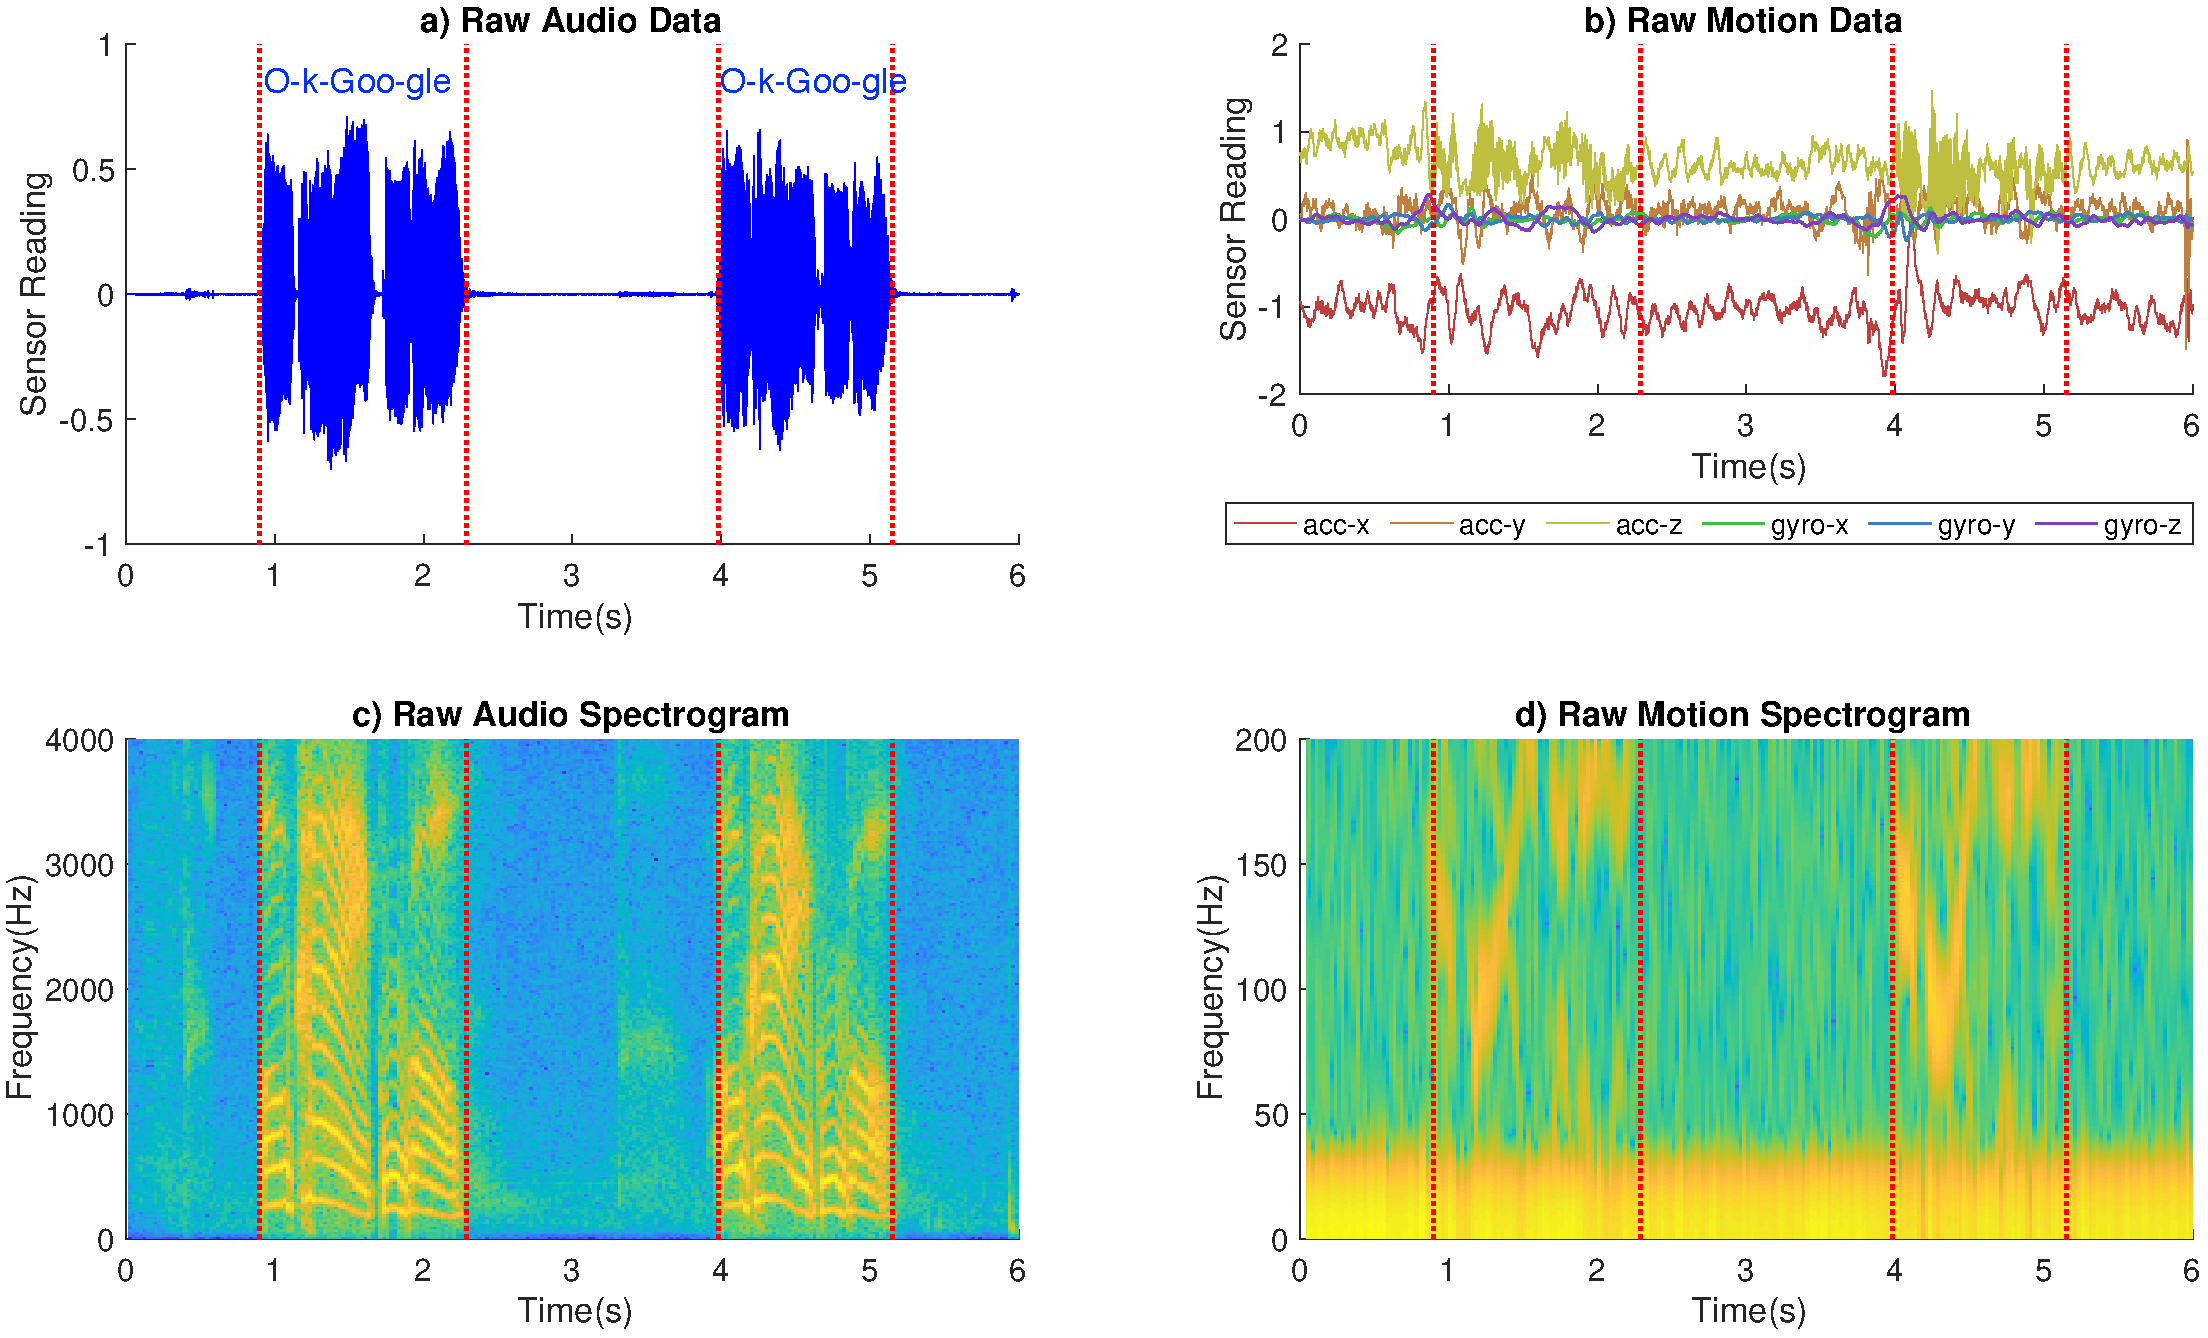
\includegraphics[height=.4\textheight]{SPSC}
%%	\caption{One user speaks ``Ok Google'' twice.}
%%	\label{fig:SPSC}
%%\end{figure}
%%%TODO more descriptions about the figure.
%%\begin{figure}[h]
%%	\centering
%%	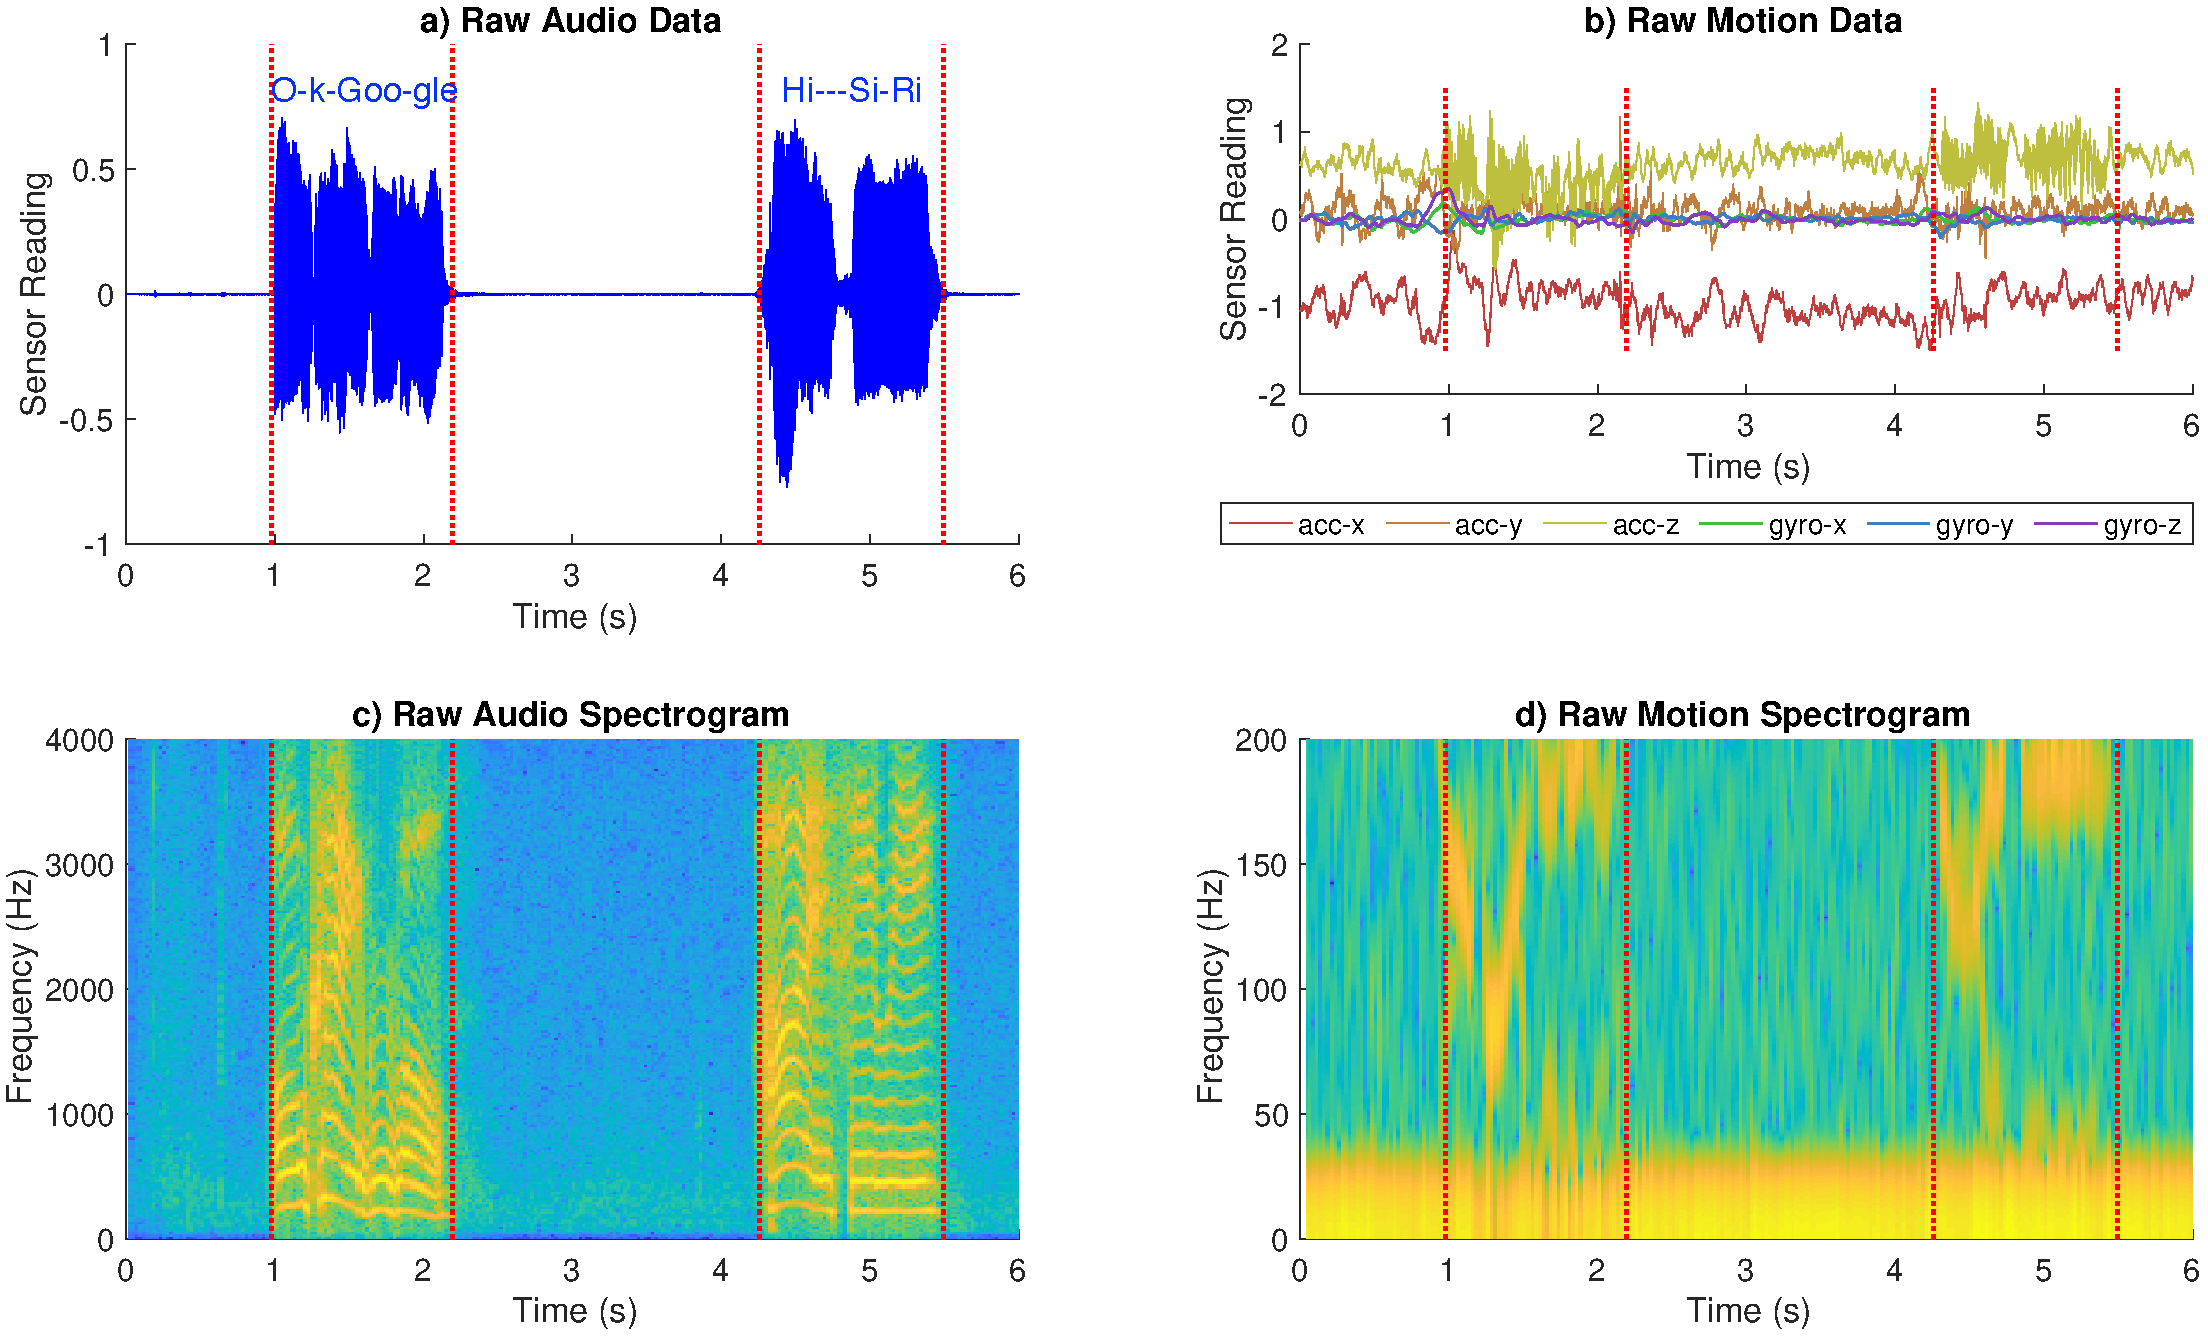
\includegraphics[height=.4\textheight]{SPDC}
%%	\caption{One user speaks ``Ok Google'' and ``Hi Siri''.}
%%	\label{fig:SPDC}
%%\end{figure}
%%\begin{figure}[h]
%%	\centering
%%	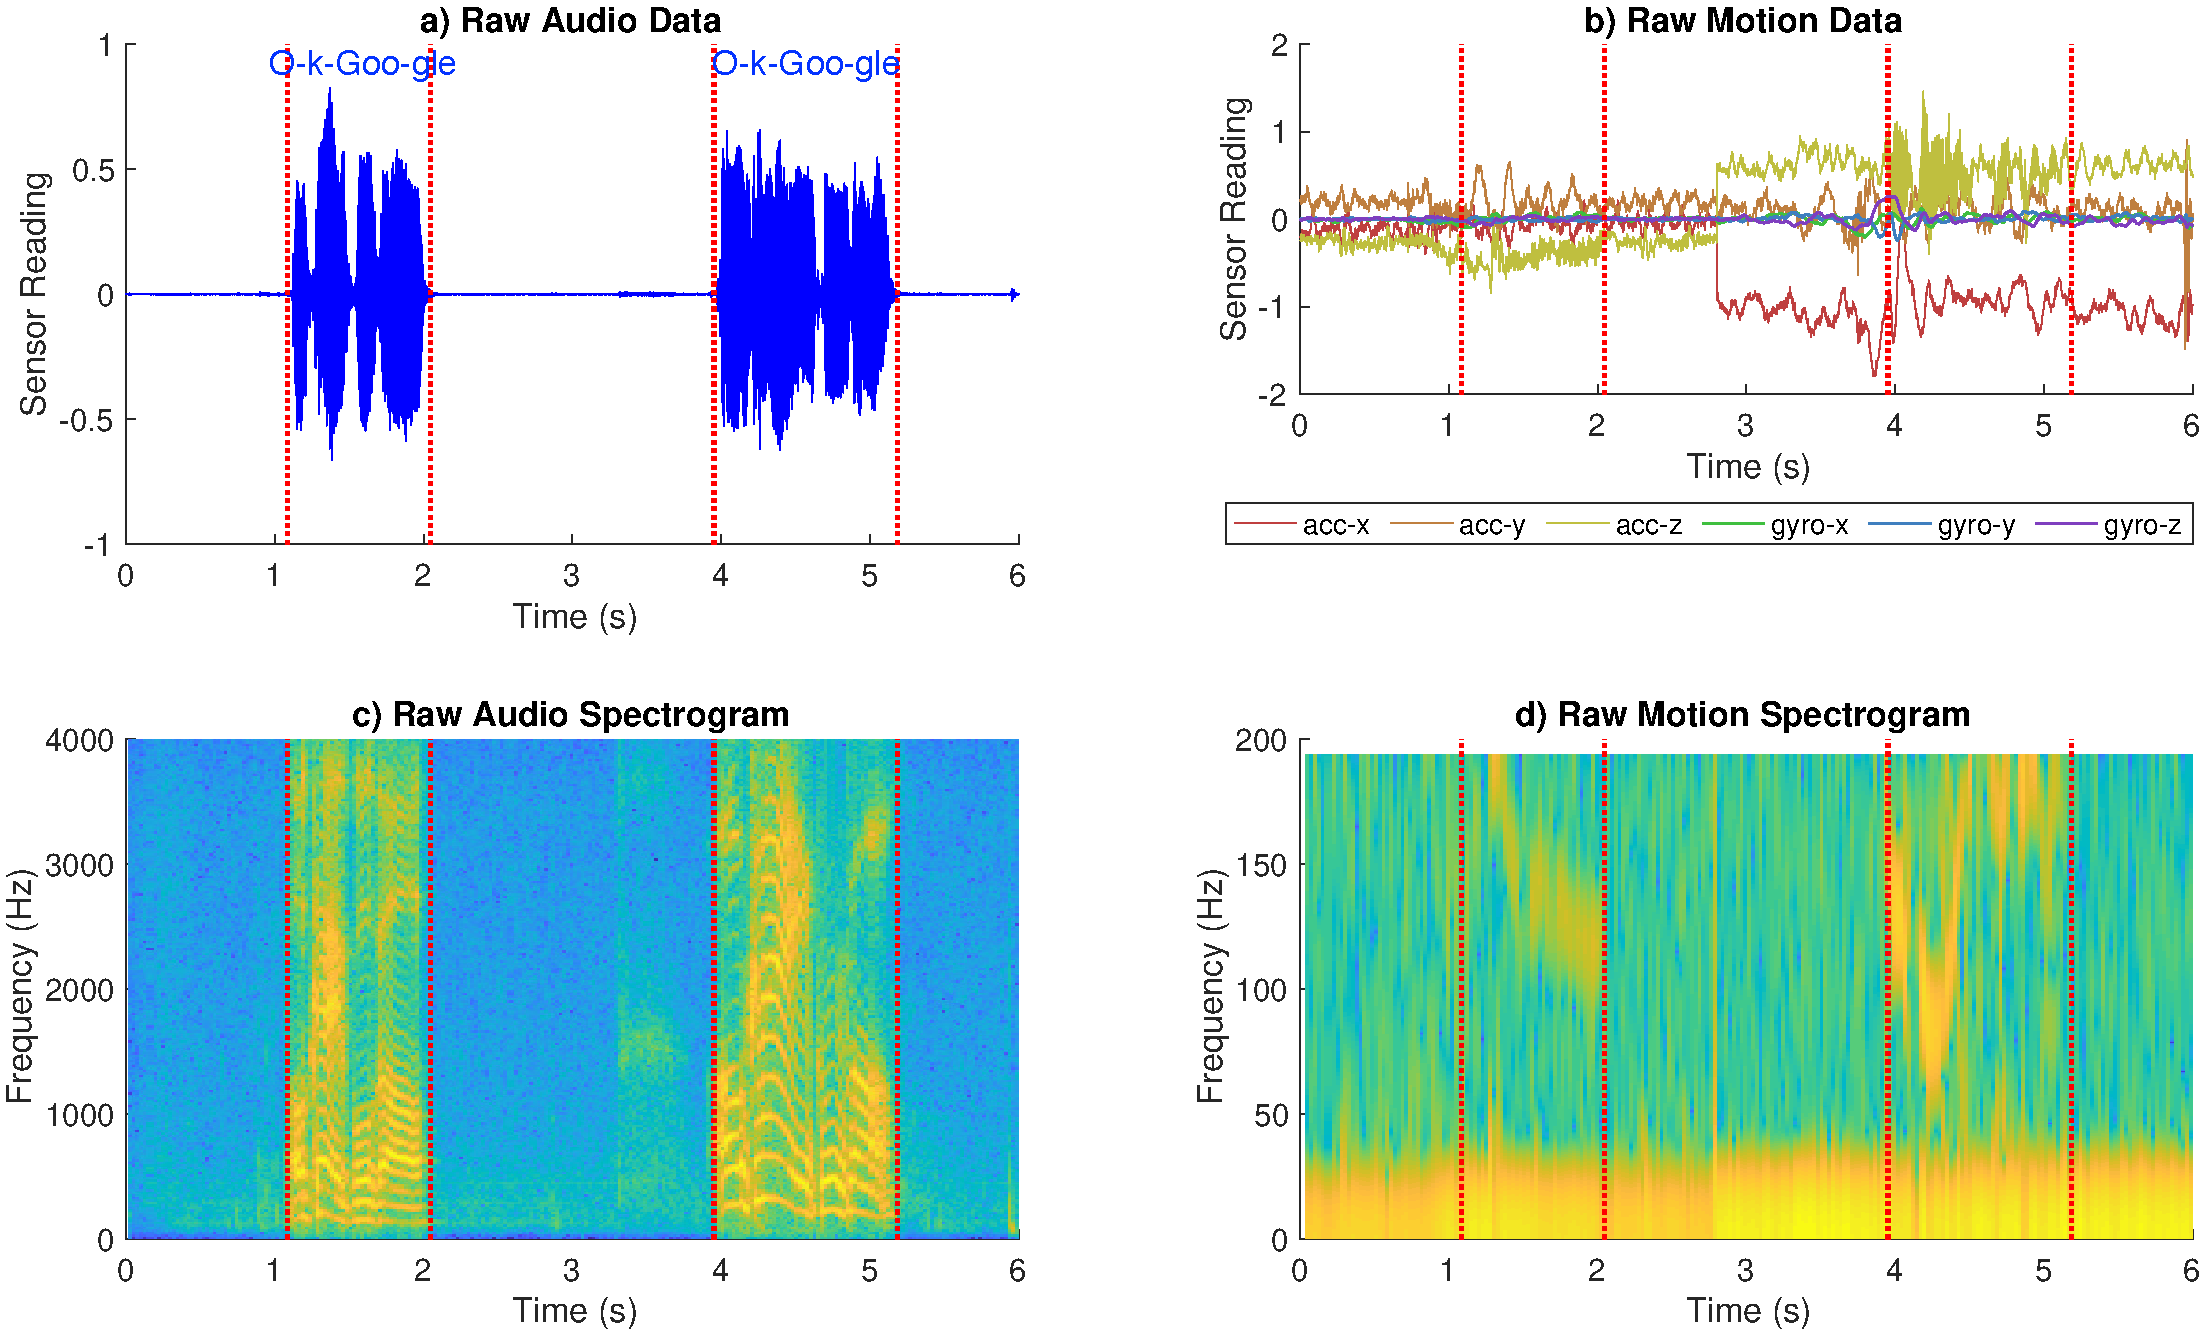
\includegraphics[height=.4\textheight]{DPSC}
%%	\caption{Different users both speak ``Ok Google''.}
%%	\label{fig:DPDC}
%%\end{figure}
%
%%TODO change same commands, do not fear DUPLICATION, ADDING HOW THE DATA IS COLLECTED
%%todo NO ()
%
%%TODO change plotted, are plotted, plot
%%WHY CHOOSE AXIS-Z
%\textbf{Proof-of-Concept}.
%Fig.~\ref{fig:SPSC}, Fig.~\ref{fig:SPDC}, and Fig.~\ref{fig:DPDC} show the example data when the same user speaks the same command ``Ok google'', the same user speaks different commands ``Ok google'' and ``Hi Siri'', and different users speak the same command ``Ok Google''. The data are collected as in Fig~\ref{fig:use}. The audio data is from the microphone with sampling rate 8,000 Hz while the motion data is sampled at 400Hz as it is the highest sample rate on Nexus 6P. In each figure, the left two subfigures, a) and c), are plotted based on microphone data, and the right two subfigures , b) and d),  are based on motion data; the top two subfigures, a) and b, plot time-domain data, while the bottom  two subfigures, c) and d), plot frequency-domain data. Note that the raw motion data have three dimensions, as shown in b) subfigures, but the spectrogram (d) subfigures only choose acc-z data to draw since it is the most representative one.
%%TODO
%
%%
%From these three figures, we can observe that the motion data are nosier and contain much fewer data and less representative than audio data, which are direct evidence of the aforementioned challenges. Note that in the ideal case, we expect when users speak the same command, no matter the same user or different users, the motion data should be similar. However, based on real data, as shown in Fig.~\ref{fig:DPDC} d), the raw spectrogram of different users are quite different. This is because different users have the different dominant speaking frequencies. What's worse, Fig.~\ref{fig:DPDC} d) shows the spectrograms are similar when one user speaks different commands.  Such observations indicate that frequency-domain data are not of much use to match between motion data and the same commands. Therefore, we adopt long short-term memory (LSTM) network, a variant of recurrent neural network (RNN), to learn the patterns of motion data in time-domain. 
%
%
%As elaborated in Section~\ref{sec:sys}, we also design syllable separation and majority voting components to further improve the performance of the LSTM network and increase the overall liveness detection accuracy.  In conclusion,  our \shortname~system has the following advantages:
%\begin{itemize}
%	\item \shortname~works with current-off-the-shelf commercial smartphones. It does not require any extra electronic device.
%	\item Except for pressing the smartphone on the user's throat, \shortname~does not ask users to do extra movements other than an ordinary speaking behavior. 
%	\item \shortname~can defend against at least 3*2= 6 different attacks. As elaborated in Section~\ref{sec:attack},  \shortname~protects the system against simple playback attack and sophisticated mimicry attack, where in each case, the speaker could play audio samples generated by replay attack, speech synthesis, or voice conversion. 
%	\item \shortname~does not require any user-specific training. Our matching algorithm is based on a user-independent model.
%	\item \shortname~currently works with text-dependent voice authentication systems. However, it is easy to expand the system to text-independent systems.
%\end{itemize}


\section{Background}

\subsection{Voice Acoustics}\label{sec:voice}

The generation of human voice follows a source-filter model~\cite{fant1960acoustic}. A speech signal can be seen as a source signal (the glottal source at the larynx, or noise generated at a constriction in the vocal tract), filtered with the resonances in the cavities of the vocal tract (tongue, teeth, lips, velum etc. modifying the sound spectrum over time). This theory has been verified using 3-D printed models of two configurations of a vocal tract to generate sounds to generate the vowels in the words ``had'' and ``heard''~\cite{wolfe2016experimentally}. 

%TODO choose one
%The fundamental frequency for speech ($f_0$) is typically 80 to 250 Hz.
A typical adult male will have a fundamental frequency  ($f_0$) of from 85 to 155 Hz, and that of a typical adult female from 165 to 255 Hz~\cite{baken1987clinical,titze1994principles}. The frequencies of the first, second and $i$-th resonances are labeled as  $R_1, R_2, \ldots R_i$, and those of the spectral peaks produced by these resonances are called formants, $F_1, F_2, \ldots F_i $~\cite{titze2015toward}. 

According to~\cite{ladefoged2014course}, English vowels are perceived largely according to the values of the formants $F_1$ and $F_2$. The range of $F_1$ is roughly from 270 to 860 Hz, and that of $F_2$ from 840 to 2790 Hz~\cite{peterson1952control}. As for English consonants, there are six categories: plosive/stop (e.g. /p/), fricative (e.g. /f/), affricate (e.g. /dZ/), nasal (e.g. /m/), lateral (e.g. /l/), and approximant (e.g. /r/). The frequencies of consonants vary a lot. The turbulence of /s/ and /z/ occurs above 3500Hz, and reaches as high as 10,000 Hz, whereas /w/ has $F_1$ from 250 to 450 Hz and $F_2 $ from 600 to 850 Hz~\cite{ladefoged2012vowels}. 

\begin{table*}[h]
	\centering
	\caption[]{Maximum Sampling Rate of Smartphone Sensors}
	%	\footnote{Some part of the data is from~\cite{matyunin2018zero}, others are tested }
	\label{tab:samplerate}
	\begin{tabular}{lccc} %{lp{2cm}p{2cm}}
		\toprule		
				\multirow{2}{3cm}{Device}& \multirow{2}{2.5cm}{Release Year } & Microphones'  & Motion Sensors'  \\
	& & Sampling Rate & Sampling Rate\footnotemark \\
		\midrule
		Samsung Galaxy S8 & 2017 & 192,000 Hz & 500 Hz\\
		Samsung Galaxy S7 & 2016 & 192,000 Hz & 500 Hz\\		
		Google Nexus 6P & 2015 & 48,000 Hz & 400 Hz\\
		LG Nexus 4 & 2012 & 48,000 Hz& 200 Hz\\
		\bottomrule
	\end{tabular}
\end{table*}
\footnotetext{Data is partially from~\cite{matyunin2018zero} and partially by calling the \texttt{getMinDelay()} function of \texttt{android.hardware.Sensor} class. In fact, the sensors can sample at a higher rate, but the operating systems restrict this rate in order to save power or for security concerns. For example, Google Nexus 6P uses Bosch BMI160, whose sampling rate can be 1600 Hz., but Android operating system only supports up to 400 Hz on the phone.}


By Nyquist–Shannon sampling theorem, to properly sample a signal contains no frequency components higher than $f$ Hz, the sampling rate must be at least $2f$ Hz (Nyquist rate). In other words, a sampling rate of 400 Hz (motion sensors' rate of Google Nexus 6P as shown in Table~\ref{tab:samplerate}) can only handle signals whose component frequencies are below 200 Hz. Except for part of the fundamentals, all $F_1$ and $F_2$ frequencies can not be sensed. Therefore, it is impossible to perceive the signals with such a low sampling rate.

Fortunately, the objective of using motion data in {\shortname} is liveness detection and user identification, not signal recovery. With some proper machine learning technology, the undersampled data is informative enough to fulfill the purpose. The reason is, in signal processing, there exists the aliasing phenomenon that high frequency data will have aliases at the low frequency range, which indicates that the information is kept, though distorted.

%Fortunately, thanks to the aliasing  phenomenon and self demodulation effect, the undersampled motion data still contains partial information, which can be used for liveness detection and user authentication .


%\subsection{Aliasing}
%Aliasing is a phenomenon that causes different signals to become indistinguishable (or aliases of one another) when sampled. For a sinusoid of frequency $f$ , sampled with frequency $f_s$, the resulting samples are indistinguishable from those of another sinusoid of frequency $\mid f − N \cdot f_s\mid$ , for any integer $N$. 
%
%Aliasing is an effect that causes different signals to become indistinguishable from each other during sampling. Aliasing is characterized by the altering of output compared to the original signal because resampling or interpolation resulted in a lower resolution in images, a slower frame rate in terms of video or a lower wave resolution in audio. Anti-aliasing filters can be used to correct this problem.


\subsection{Self Demodulation}
Motion sensors not only captures the original sound data, but also captures the modulated signals. In detail, with self demodulation~\cite{berktay1965possible}, the original sounds self interacts  inside  human body,  resulting in sounds with  lower frequency.

\begin{figure}[h]
	\centering
		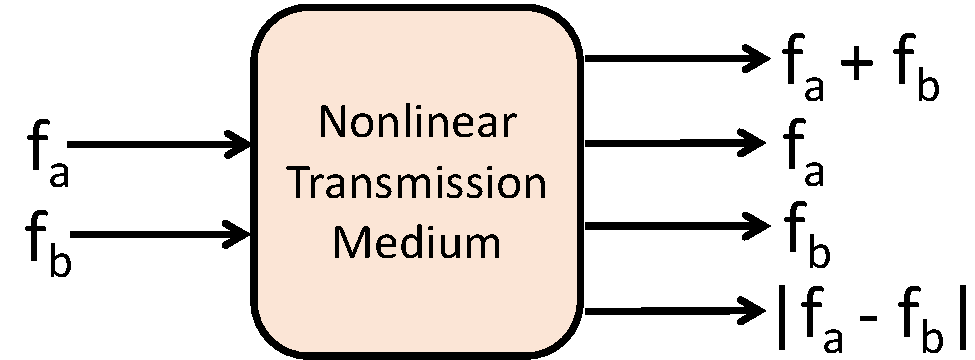
\includegraphics[width=.6\linewidth]{modulation}
	\caption{Self Demodulation of Sound Signals  When Transmitting Through the Human Body.}
	\label{fig:modulation}
\end{figure}

Researchers have found that sounds with different frequencies that transmitted through a nonlinear medium would interact with each other~\cite{pompei1998use}. This interaction produces new frequencies upon the combination of the sums and differences of the individual frequency components by Khokhlov-Zabolotskaya-Kuznetsov(KZK) parabolic nonlinear wave equation~\cite{novikov1987nonlinear}. 

Since the acoustic impedance of the human body is similar to that of water~\cite{kim2014sound}, the self-demodulation would occur in the human body as show in Fig.~\ref{fig:modulation}. 
The original sound signals with frequency $f_a$ and $f_b$ would introduce two more signals with frequency $f_a + f_b$ and $|f_a - f_b|$. For different person, the original signals generated have different frequency, so the low frequency signal $|f_a - f_b|$ are different, which can be utilized for user authetication.
%
Moreover, note that electronic devices has different acoustic property from that of human body. Therefore, those low frequent signals can be used for liveness detection.

%However, borrowing theories from \textit{compressed sensing}, the {\systemName} system can partially reconstruct the signal and obtain critical information such as the numbers appeared in a conversation, genders or even identities of the speakers, etc., from motion sensor readings, as discussed in Section~\ref{sec:threat}.

\subsection{Acoustic Attenuation}
Another effect helps {\shortname} to do spoof-proof authentication is the acoustic attenuation by human body.
%
It is known that human voice is emitted by the vocal organ and is a combination of mechanical vibrations with multiple  amplitudes and different  frequencies.
%
When a person speaks, the  airflow from the lungs through the trachea compresses the vocal cords causing vibrations to make sounds. The lung, trachea and vocal cord form a resonance chamber. 
%\begin{figure}[h]
%	\centering
%		\includegraphics[width=.4\linewidth]{background}
%	\caption{Background}
%	\label{fig:background}
%\end{figure}

Suppose the length of vocal cords is $d$, the lung volume is $V_0$ and the cross-sectional area at the vocal cords is $S$. According to the polytropic process equation, when the airflow moves $d$, the air pressure at the vocal cords can be expressed as follows,
\begin{displaymath}
P_1 = \frac{P_0 \cdot V^\gamma_0 }{(V_0 - d \cdot S)^\gamma},
\end{displaymath}
where $P_0$ is the normal atmospheric pressure, and $\gamma$ is a coefficient about the air specific heat. 
According to the definition of pressure, if the area at the vocal cords is $S_v$,  the force at the vocal cord is,
\begin{displaymath}
F_0 = P_1 \cdot S_v = \frac{S_v \cdot P_0 \cdot V^\gamma_0 }{(V_0 - d \cdot S)^\gamma}.
\end{displaymath}
When the force is applied to the vocal cords, vertical displacement occurs. 
According to the Newton’s second law of motion, we have,
\begin{displaymath}
F(t) = m a(t) + k x(t) + c v(t),
\end{displaymath}
where $F(t)$ is the external force, $v(t)$ is the speed, $x(t)$ is the vertical displacement, $c$ is the damping coefficient, and $k$ is the spring constant and m is the mass. 
The relation can further be explained as,
\begin{equation}
F(t) = m \frac{d^2 x(t)}{d t^2} + k x(t) + c \frac{x(t)}{d t}.
\label{eq:force}
\end{equation}

The vibration during an airflow pass the vocal cords can be separated into two phases. In the first phase, the airflow is passing the vocal cords which is considered to be a forced vibration with constant force $F_0$. After the airflow passed, in the second phase, the pressure of airflow disappears which leaves the system to vibrate on its own and this is called free vibration. In the forced vibration phase, after applying the Fourier transform to both side of e.q.~\eqref{eq:force}, we have,
\begin{displaymath}
\frac{F_0}{j \omega}(1-e^{-j\omega \delta t}) = - \omega^2 m X(\omega) + k X(\omega) + j \omega c X(\omega).
\end{displaymath}
That is,
\begin{displaymath}
X(\omega) = \frac{1-e^{-j\omega \delta t}}{-\frac{j m}{F_0} \omega^3 - \frac{c}{F_0} \omega^2 + \frac{j k}{F_0} \omega},
\end{displaymath}
where $X(\omega)$ is the spectrum of the vertical vibration signal and $\omega$ is the frequency. 
During the horizontal propagation of the vibration signal from the vocal cords to the throat, the vibration suffers from attenuation, and the corresponding model can be stated as follows,
\begin{displaymath}
x_s(t) = x(t) e^{-\alpha d},
\end{displaymath}
where $x_s(t)$ is the vertical displacement at the throat where the vibration has propagated, $x(t)$ is the vertical displacement at the vocal cords, $d$ is the propagation distance, and $\alpha$ is the attenuation coefficient. 
After applying the Fourier transform to both side of e.q.~\eqref{eq:force}, we have,
\begin{displaymath}
X_s(\omega) = X(\omega) e^{-\alpha d}.
\end{displaymath}
Note that $\alpha$ is related to the propagation medium. Wave propagation in body is dispersive by nature, which implies that different frequencies propagate with different attenuation coefficients at different velocities. Roughly speaking, the attenuation is small when the vibration signal propagates through the hard bone, whereas the attenuation is large through the soft tissue. Therefore, vibration waves generated at different positions at throat result in different values of $\alpha$ and $d$, which make the vibration signals unique at different positions. 
After putting all equations together, we obtain,
\begin{displaymath}
X_s(\omega) = \frac{(1-e^{-j\omega \delta t}) e^{-\alpha d}}{(-jm\omega^3 - c \omega^2 + jk\omega)(\frac{(V_0 - d \cdot S)^\gamma}{S_v \cdot P_0 \cdot V^\gamma_0 })}.
\end{displaymath}
For the same location of the human body, $m$, $c$ and $k$ are stable and belong to the same biometric feature. Each person’s lung volume and vocal cords are also different. Therefore, the vibration at the throat of different people can uniquely be identified, which can be leveraged for authentication. The propagation from electronic device to the target smartphone is different from vocal organ through human body. Thus, this effect is also valuable for liveness detection.


%\subsection{Voice Production}
%source-filter model, why our algorithm is user-independent. Similar source, different filter.
%\subsection{Voice Authentication System}
%Attacking (direct/indirect), here we only consider direct.



\section{Proof-of-Concept}
We test the feasibility of {\shortname} and the results are shown from Fig.~\ref{fig:SPSC} to Fig.~\ref{fig:device}. In each figure, we show both the raw signal and the spectrogram for the microphone data and the motion sensor data. All data are collected by Google Nexus 6P. The audio data is sampled at 8,000 Hz (telephone quality) while the motion data is sampled at 400 Hz as it is the highest sampling rate on Nexus 6P.


Fig.~\ref{fig:SPSC}, Fig.~\ref{fig:DPSC} and Fig.~\ref{fig:SPDC}, show the example data when the same user speaks the same command ``Ok Google'', different users speak the same command ``Ok Google'', and the same user speaks different commands ``Ok Google'' and ``Hi Siri'', respectively. The data are collected as in Fig~\ref{fig:usec}. In each figure, the top subfigure (a) is the raw microphone data; the subfigure (b) contains the 3-axis accelerometers data and 3-axis gyroscopes data; the subfigure (c) shows the frequency-domain information of raw audio data while the subfigure (d) show that of raw motion data. In subfigure (d), we only choose acc-z data to draw since it is the most representative one. The vertical red lines demonstrate the start and end points of the sounding period.

\newpage
%TODO figures about challenges
\begin{figure}[H]
	\centering
	\begin{minipage}[t]{.8\linewidth}
		\centering
		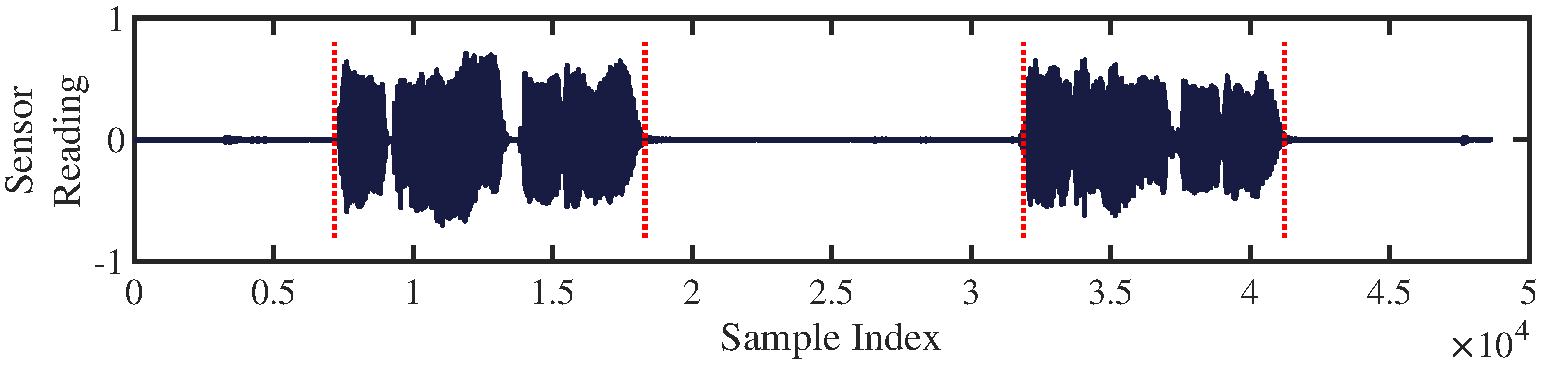
\includegraphics[width=\linewidth]{SPSC0}
		\vspace{-.2in}
		\subcaption{Raw Audio Data.}
		\vspace{.2in}
		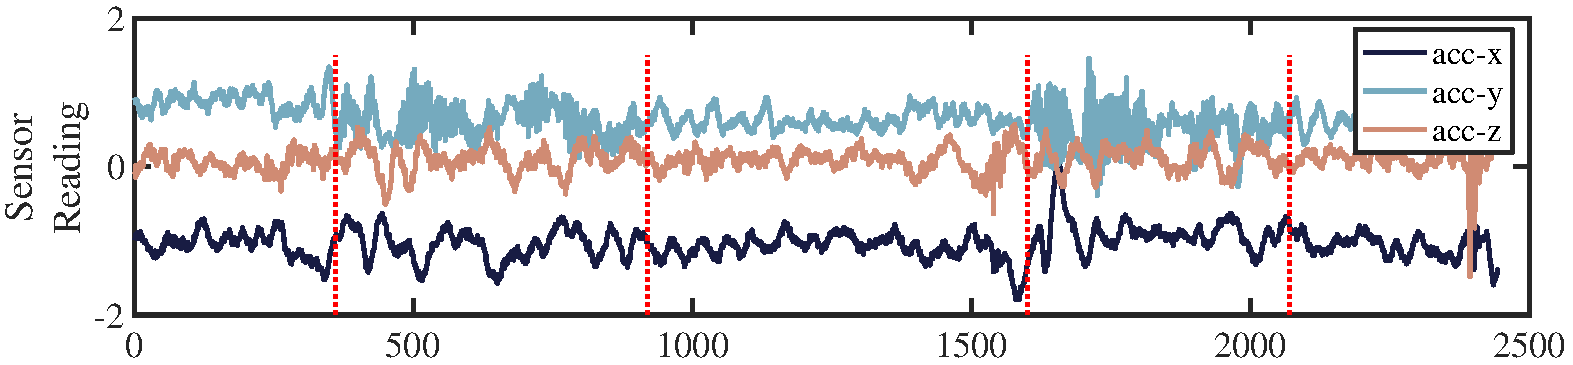
\includegraphics[width=\linewidth]{SPSC1}
		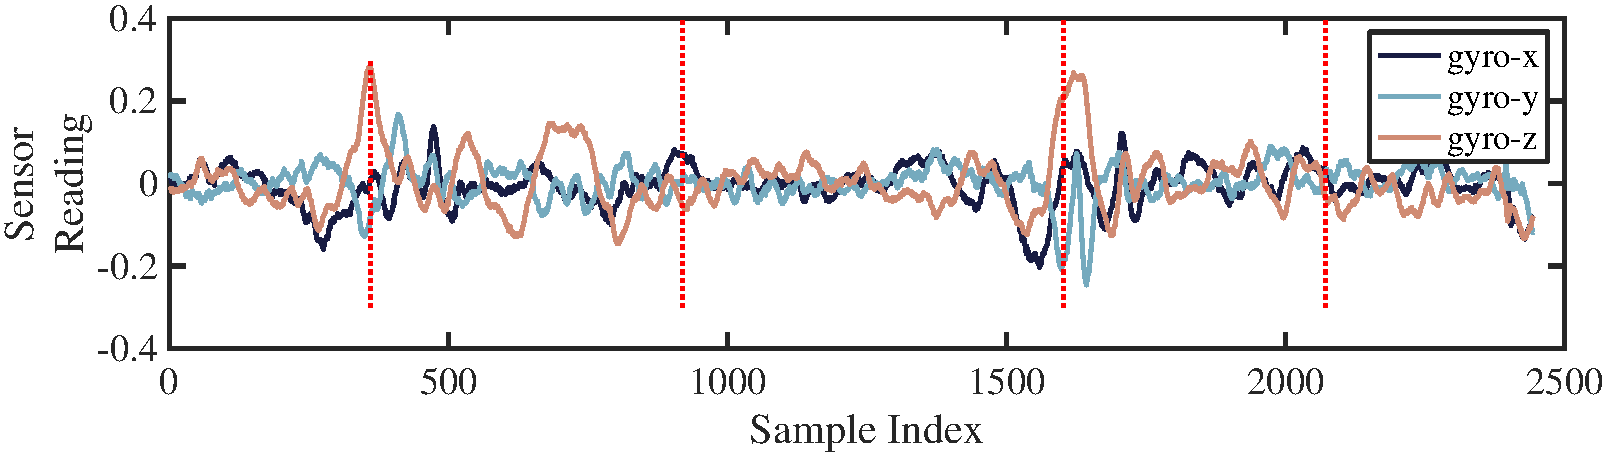
\includegraphics[width=\linewidth]{SPSC2}
		\vspace{-.2in}
		\subcaption{Raw Motion Data.}
		\vspace{.2in}
	\end{minipage}
	\begin{minipage}[t]{.45\linewidth}
		\centering
		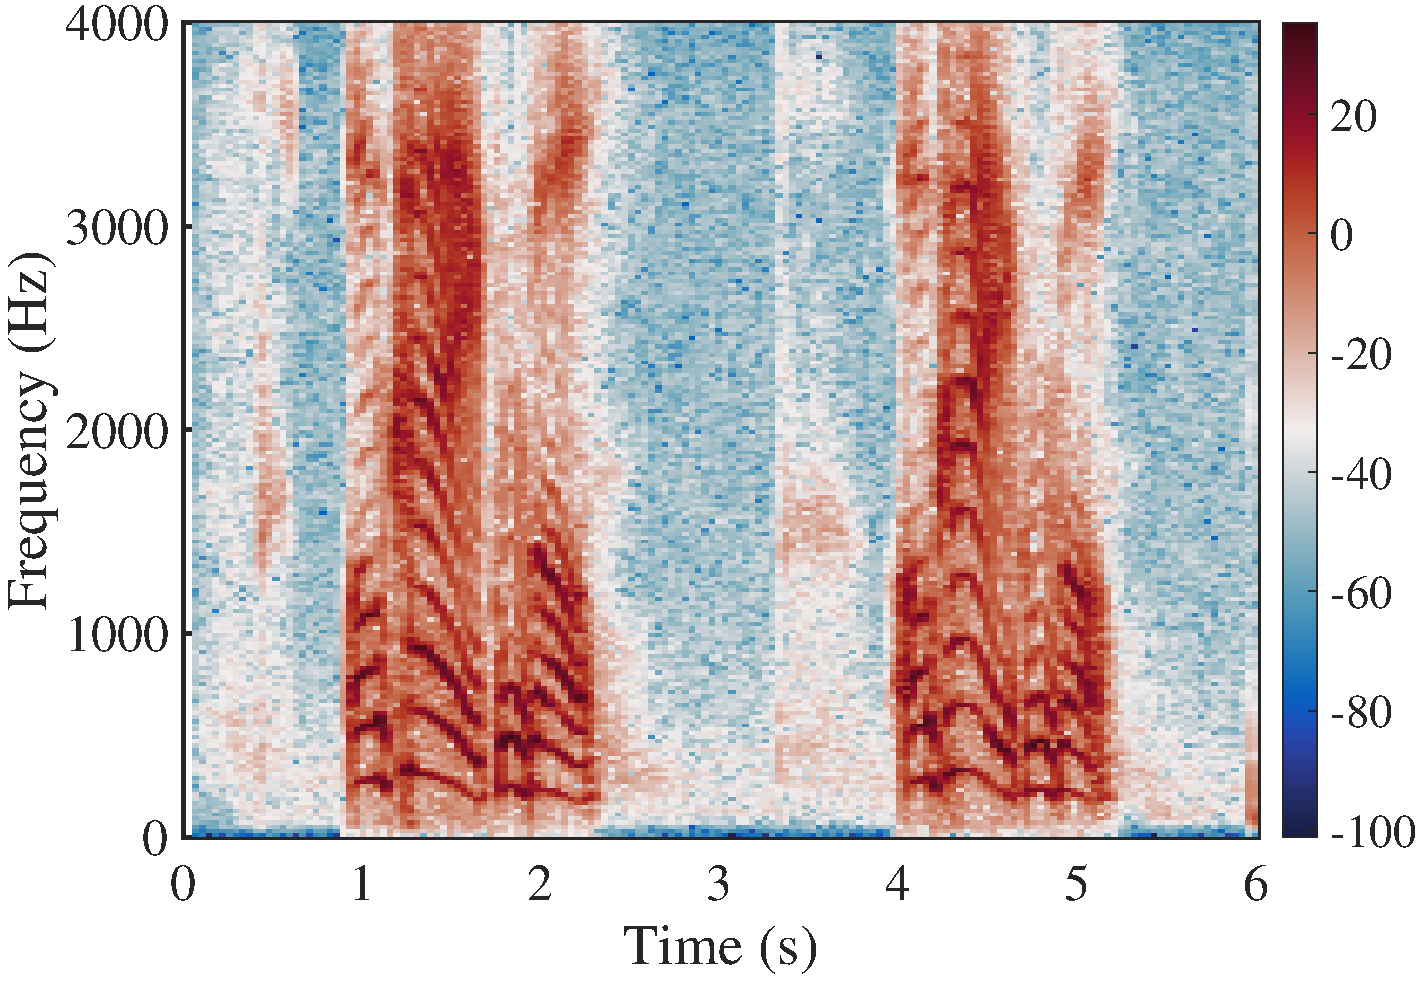
\includegraphics[width=\linewidth]{SPSC3}
		\vspace{-.2in}
		\subcaption{Spectrogram of Raw Audio Signals.}
	\end{minipage}
	\begin{minipage}[t]{.45\linewidth}
		\centering
		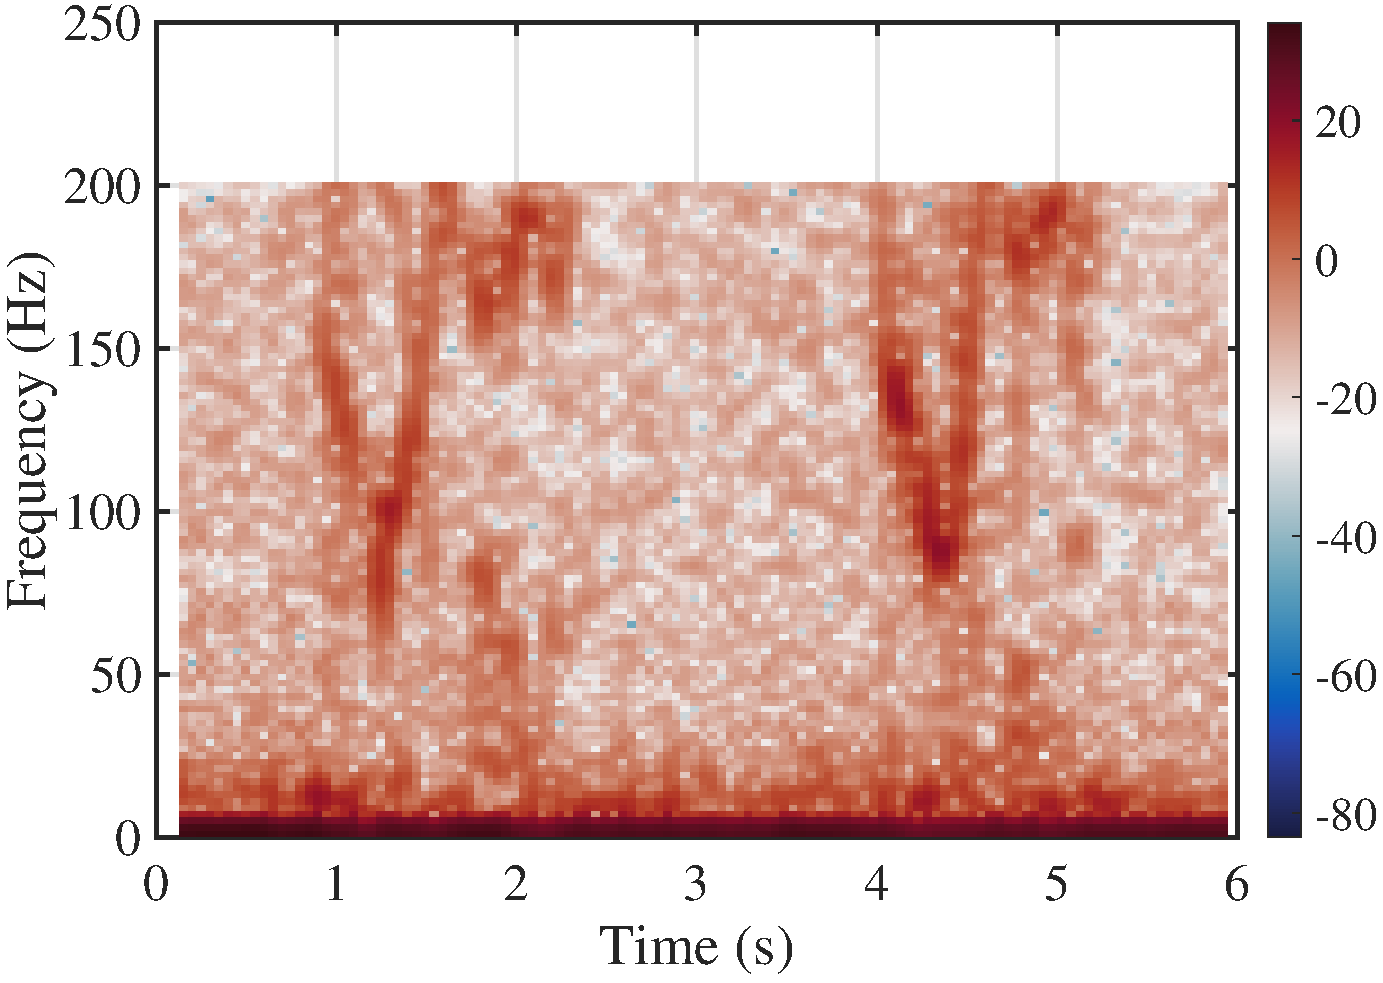
\includegraphics[width=\linewidth]{SPSC4}
		\vspace{-.2in}
		\subcaption{Spectrogram of Raw Motion Signals.}
	\end{minipage}
	\caption{One user speaks ``Ok Google'' twice.}
	\label{fig:SPSC}
\end{figure}
%
\newpage
\begin{figure}[H]
	\centering
	\begin{minipage}[t]{.8\linewidth}
		\centering
		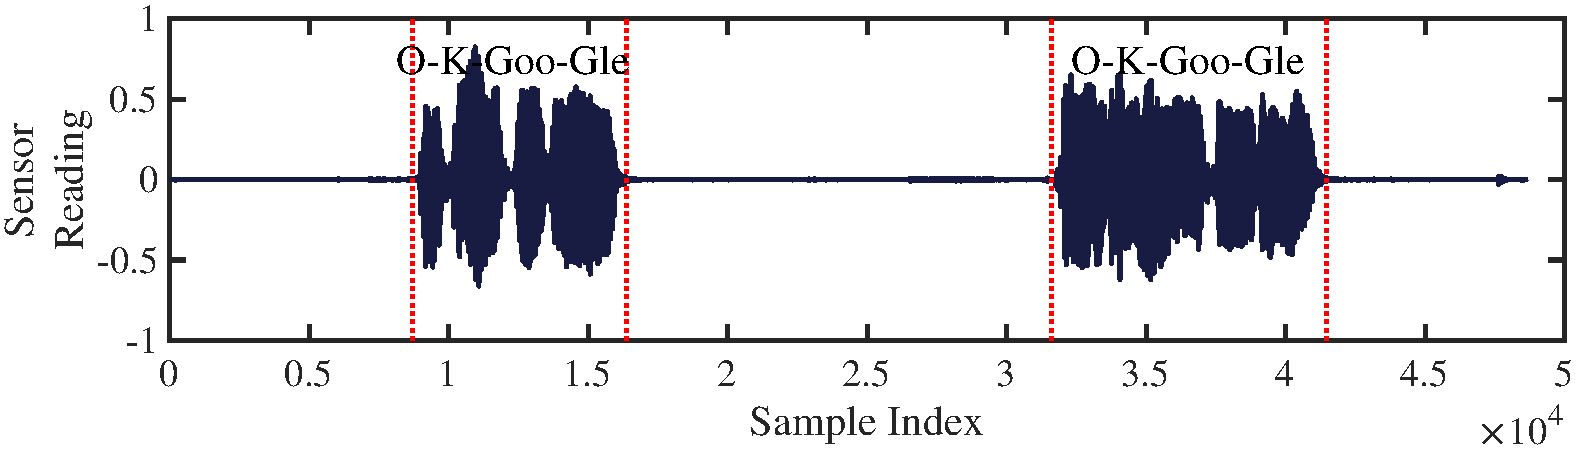
\includegraphics[width=\linewidth]{DPSC0}
		\vspace{-.2in}
		\subcaption{Raw Audio Data.}
		\vspace{.2in}
		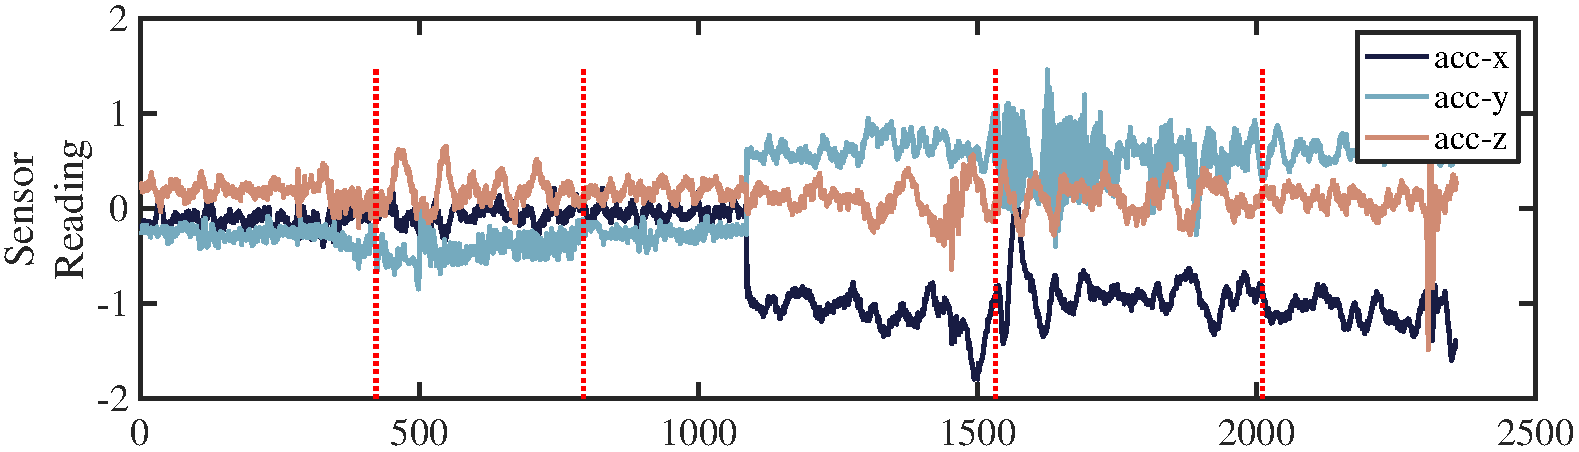
\includegraphics[width=\linewidth]{DPSC1}
		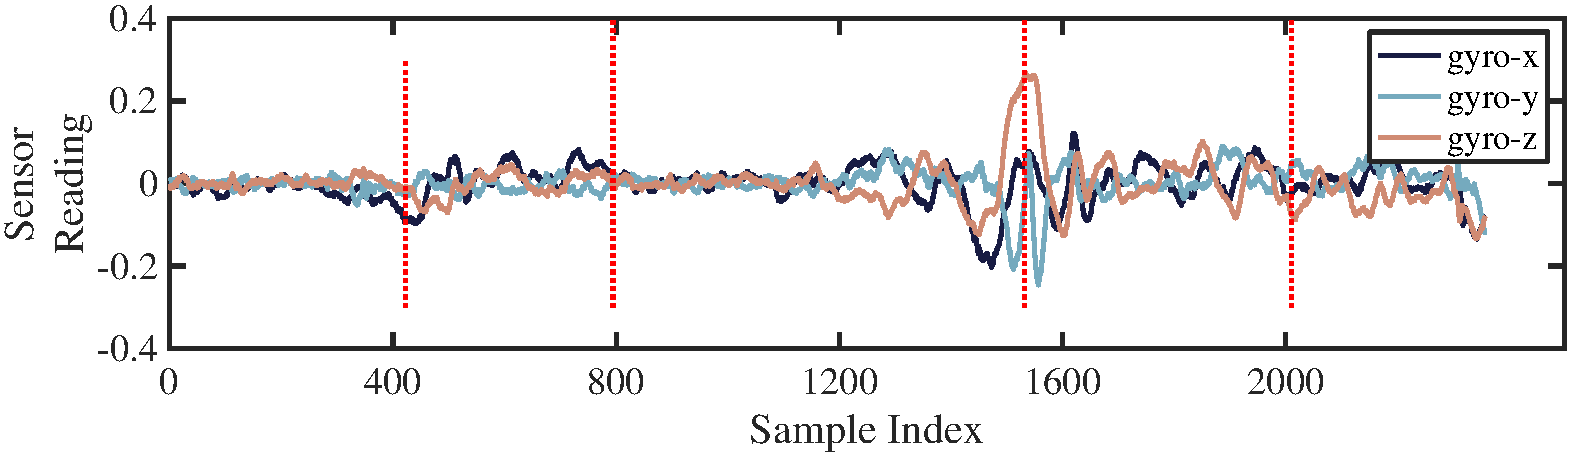
\includegraphics[width=\linewidth]{DPSC2}
		\vspace{-.2in}
		\subcaption{Raw Motion Data.}
		\vspace{.2in}
	\end{minipage}
	\begin{minipage}[t]{.45\linewidth}
		\centering
		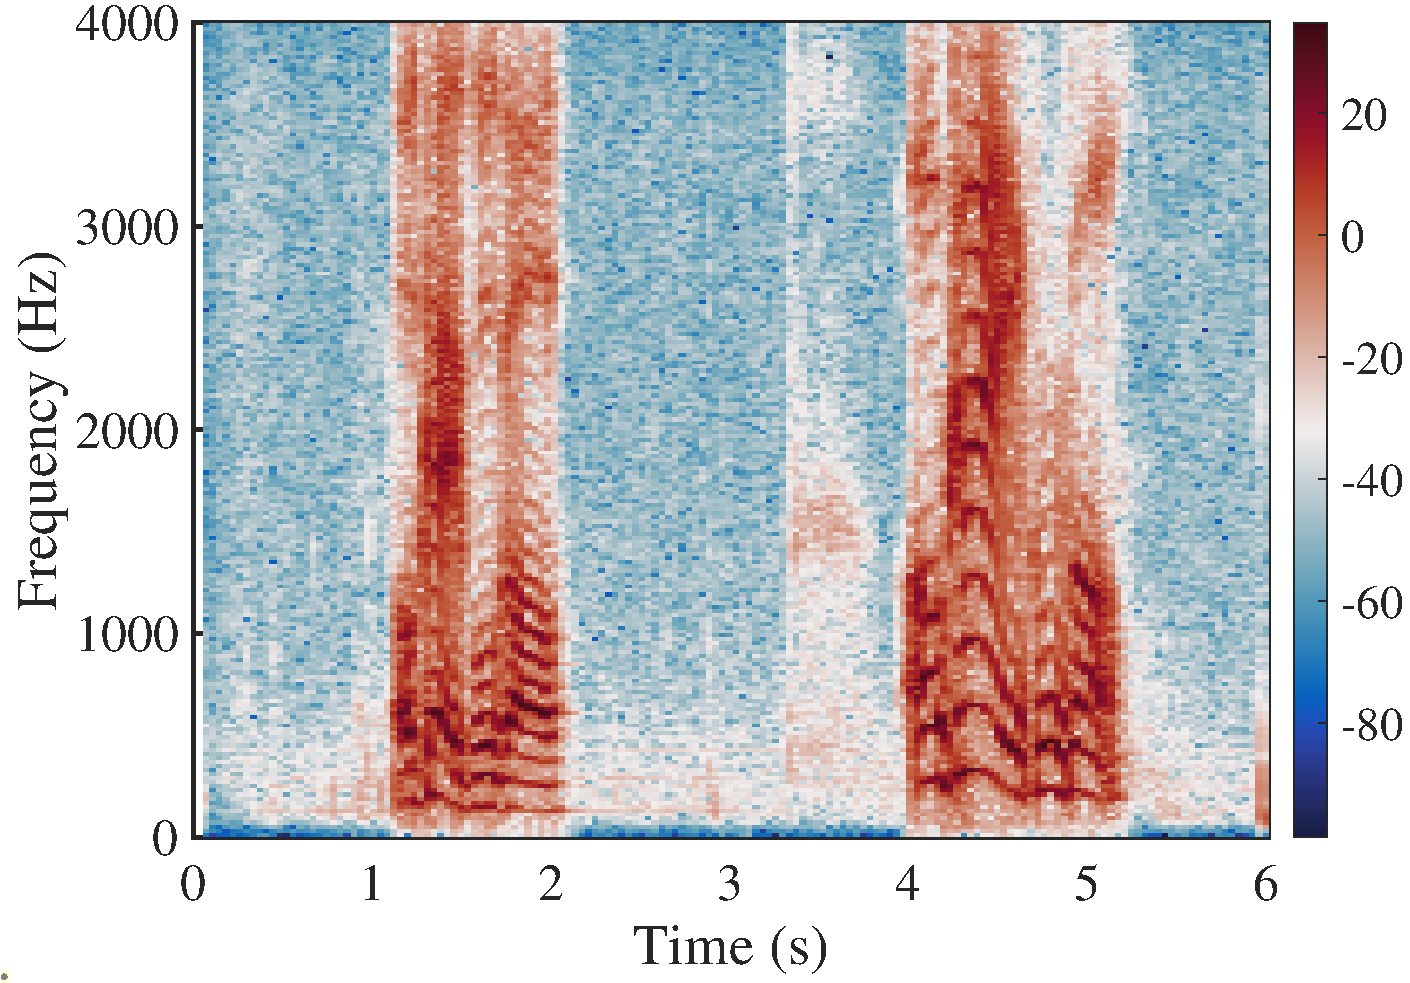
\includegraphics[width=\linewidth]{DPSC3}
		\vspace{-.2in}
		\subcaption{Spectrogram of Raw Audio Signals.}\label{fig:DPSCc}
	\end{minipage}
	\begin{minipage}[t]{.45\linewidth}
		\centering
		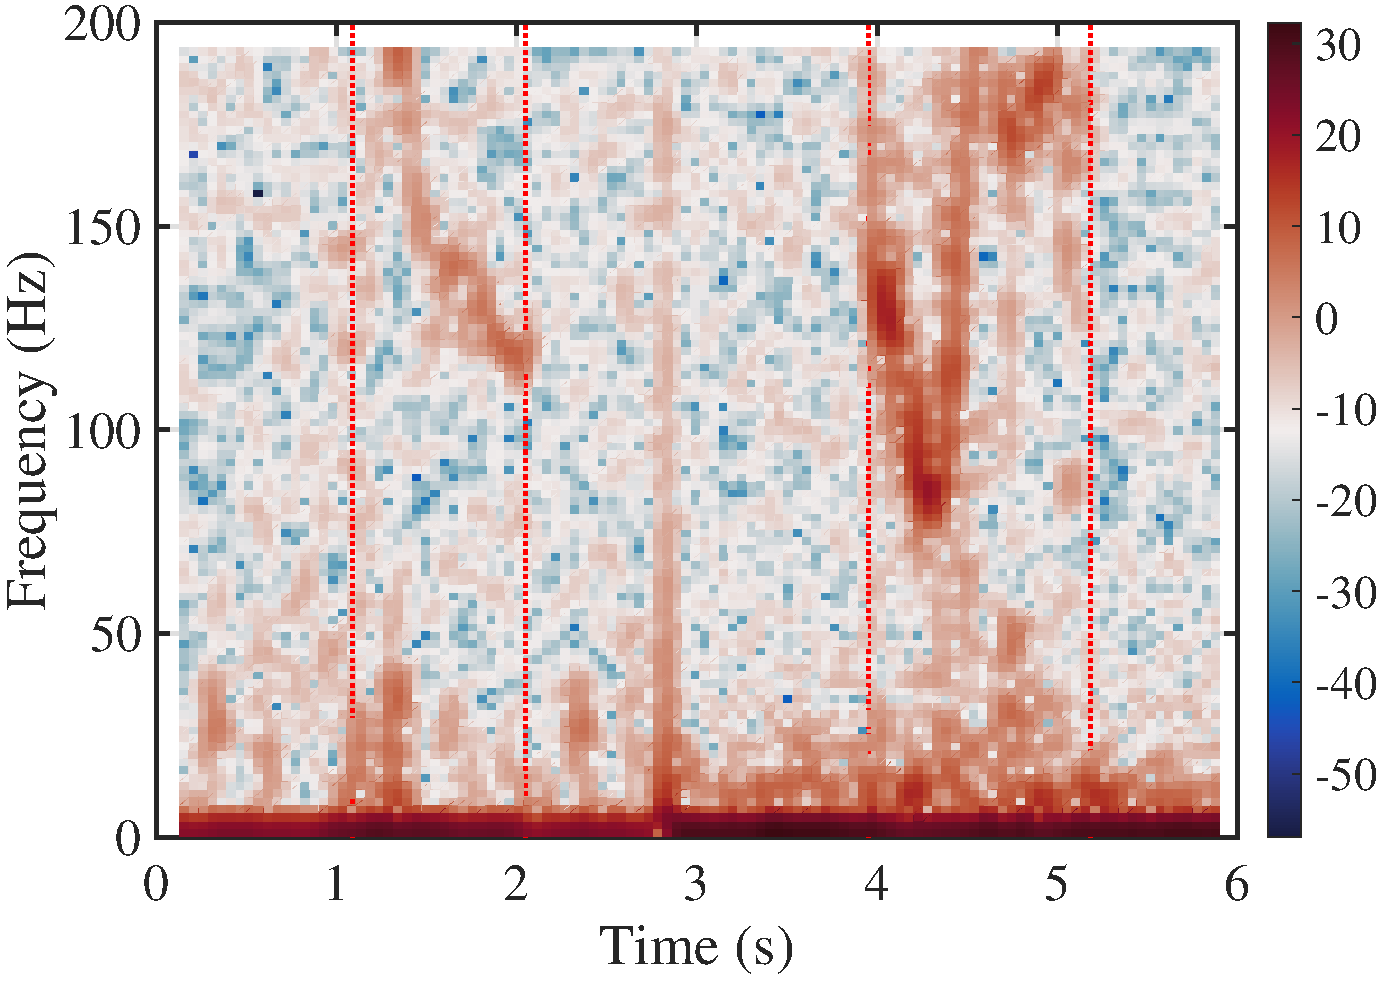
\includegraphics[width=\linewidth]{DPSC4}
		\vspace{-.2in}
		\subcaption{Spectrogram of Raw Motion Signals.}\label{fig:DPSCd}
	\end{minipage}
	\caption{Different users both speak ``Ok Google''.}
	\label{fig:DPSC}
\end{figure}
%TODO more descriptions about the figure.
\newpage
\begin{figure}[H]
	\centering
	\begin{minipage}[t]{.8\linewidth}
		\centering
		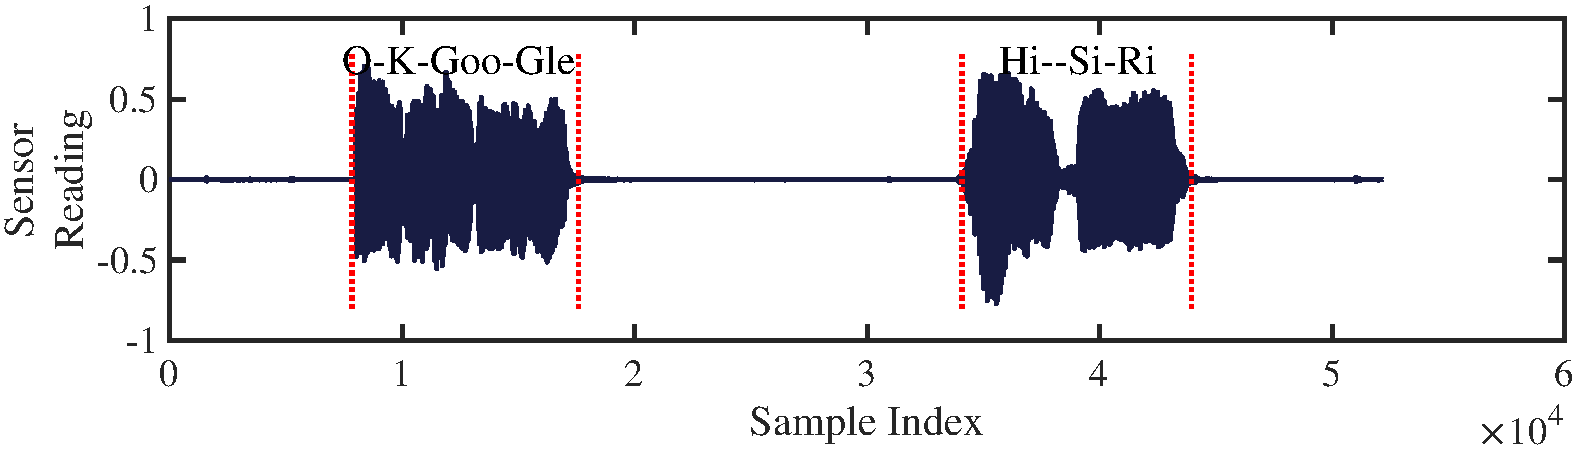
\includegraphics[width=\linewidth]{SPDC0}
		\vspace{-.2in}
		\subcaption{Raw Audio Data.}
		\vspace{.2in}
		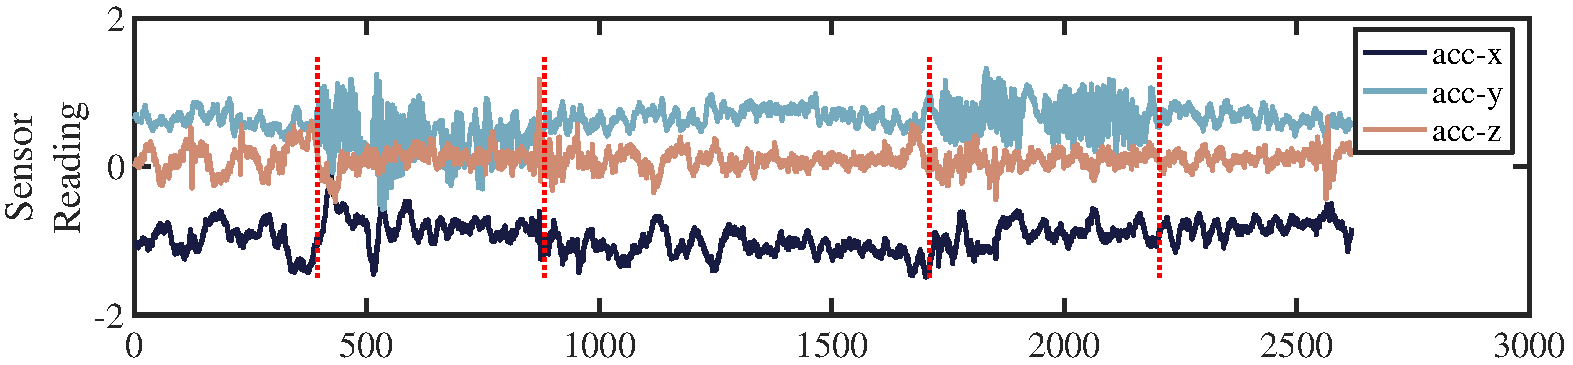
\includegraphics[width=\linewidth]{SPDC1}
		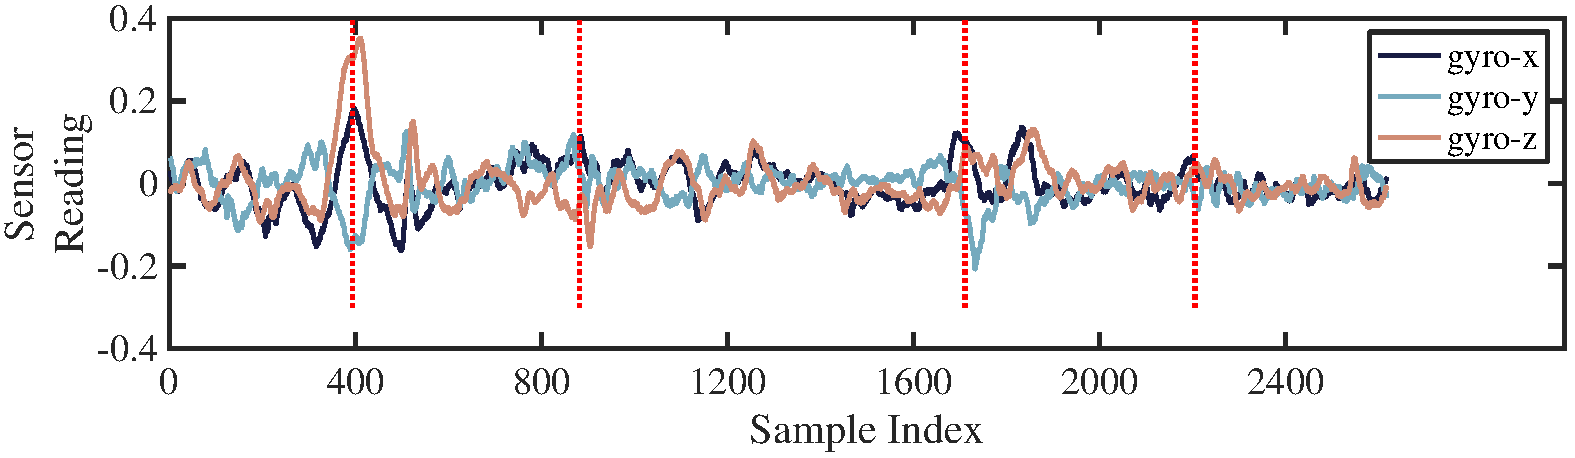
\includegraphics[width=\linewidth]{SPDC2}
		\vspace{-.2in}
		\subcaption{Raw Motion Data.}
		\vspace{.2in}
	\end{minipage}
	\begin{minipage}[t]{.45\linewidth}
		\centering
		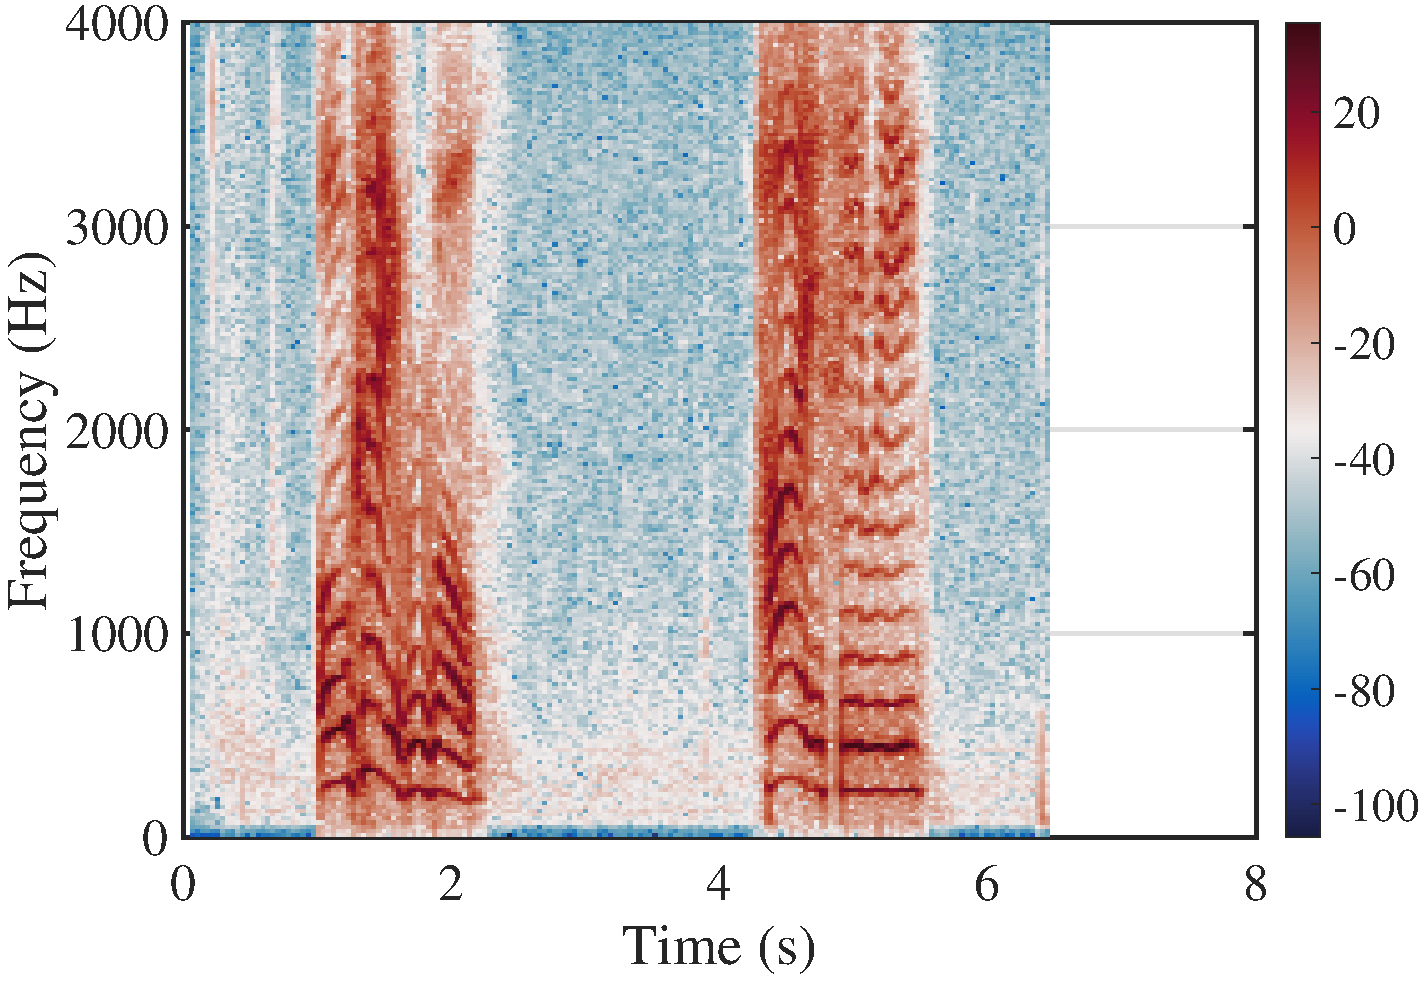
\includegraphics[width=\linewidth]{SPDC3}
		\vspace{-.2in}
		\subcaption{Spectrogram of Raw Audio Signals.}
	\end{minipage}
	\begin{minipage}[t]{.45\linewidth}
		\centering
		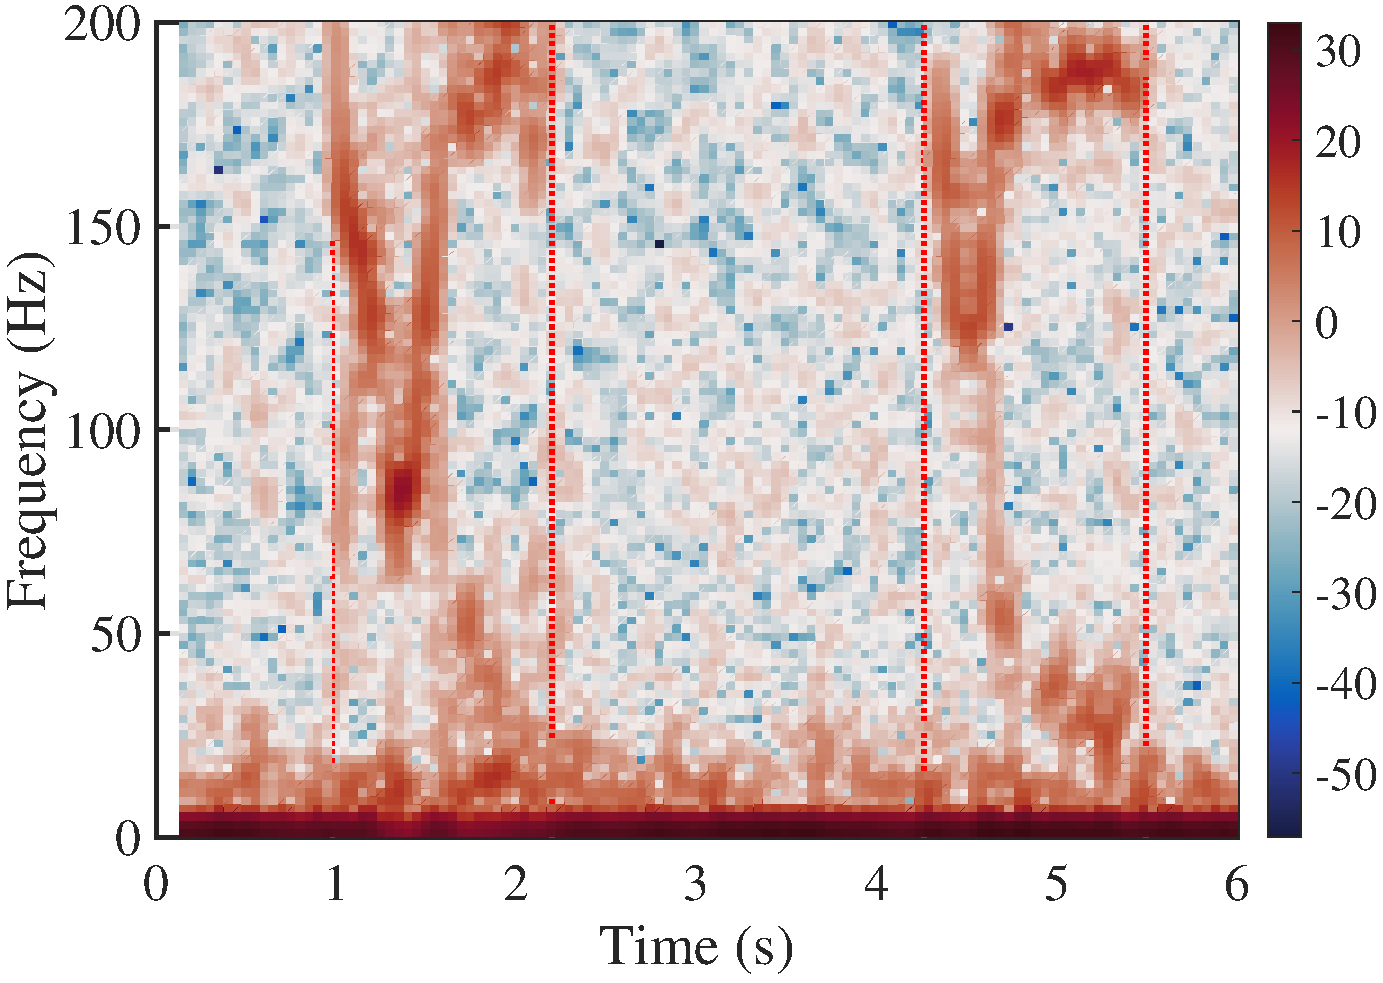
\includegraphics[width=\linewidth]{SPDC4}
		\vspace{-.2in}
		\subcaption{Spectrogram of Raw Motion Signals.}
	\end{minipage}
	\caption{One user speaks ``Ok Google'' and ``Hi Siri''.}
	\label{fig:SPDC}
\end{figure}
\newpage
\begin{figure}[H]
	\centering
	\begin{minipage}[t]{.8\linewidth}
		\centering
		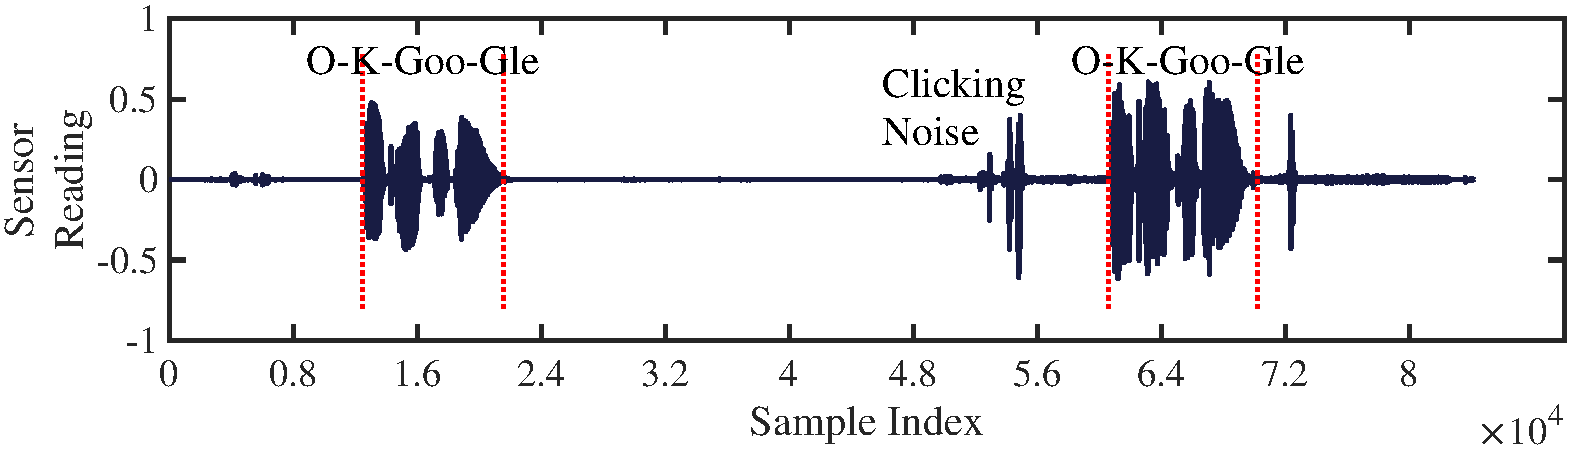
\includegraphics[width=\linewidth]{Device0}
		\vspace{-.2in}
		\subcaption{Raw Audio Data.}
		\vspace{.2in}
		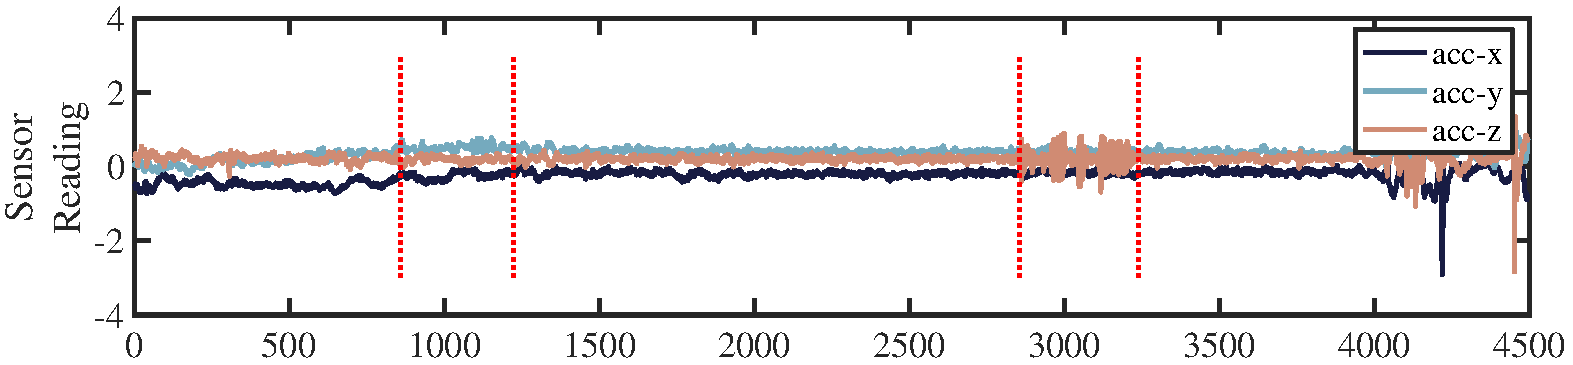
\includegraphics[width=\linewidth]{Device1}
		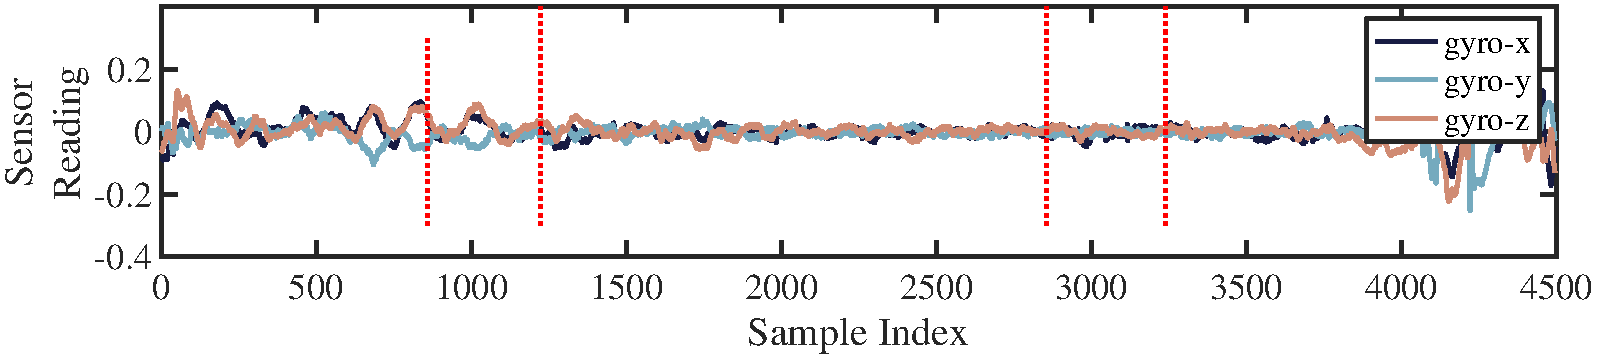
\includegraphics[width=\linewidth]{Device2}
		\vspace{-.2in}
		\subcaption{Raw Motion Data.}
		\vspace{.2in}
	\end{minipage}
	\begin{minipage}[t]{.45\linewidth}
		\centering
		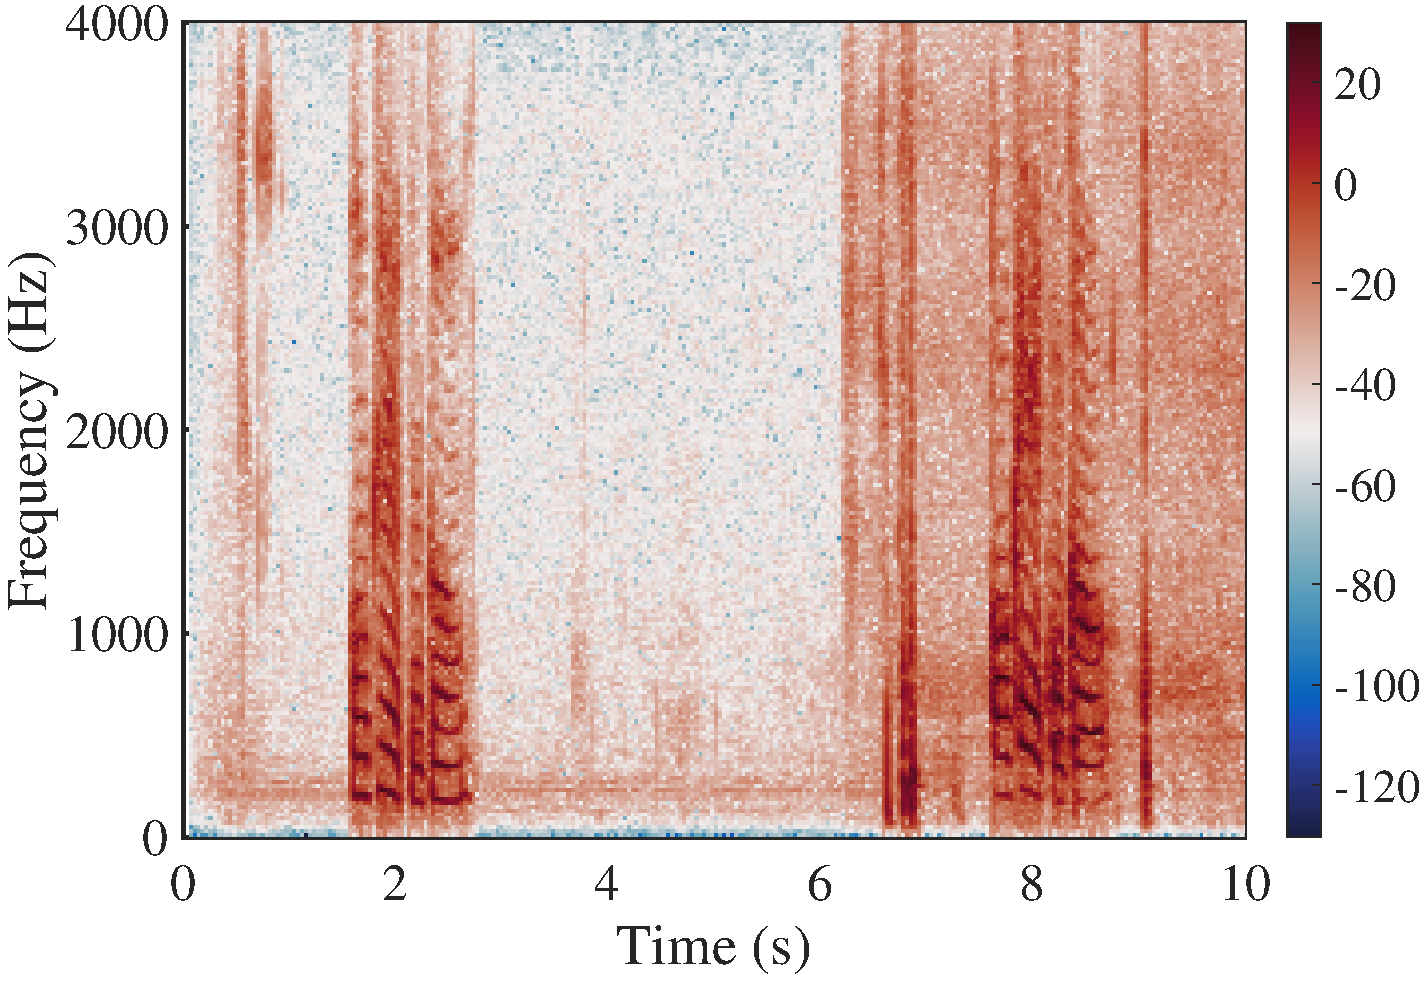
\includegraphics[width=\linewidth]{Device3}
		\vspace{-.2in}
		\subcaption{Spectrogram of Raw Audio Signals.}
	\end{minipage}
	\begin{minipage}[t]{.45\linewidth}
		\centering
		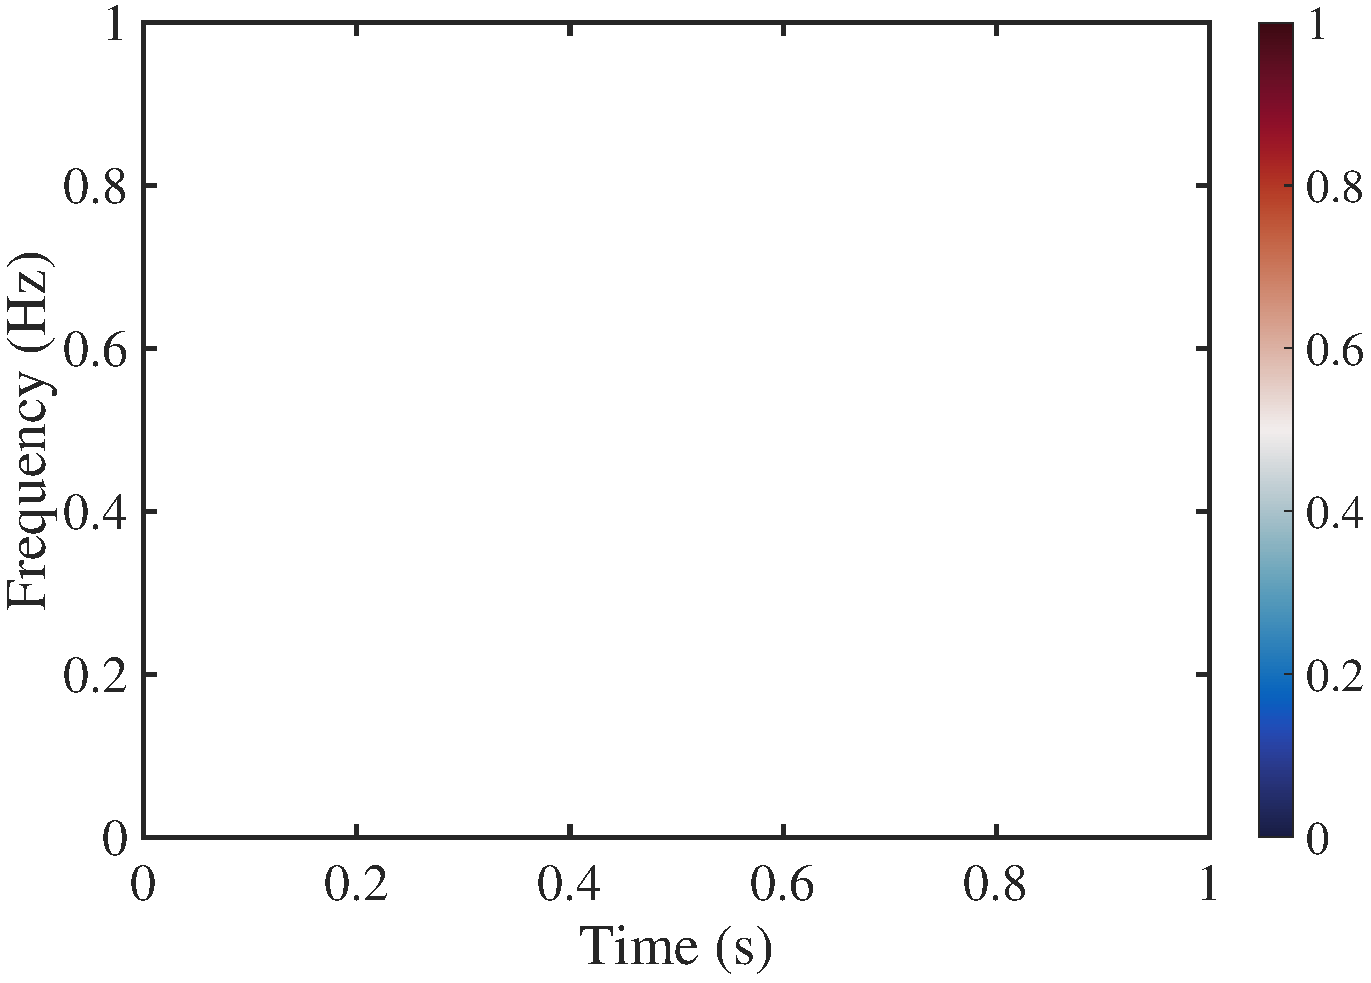
\includegraphics[width=\linewidth]{Device4}
		\vspace{-.2in}
		\subcaption{Spectrogram of Raw Motion Signals.}\label{fig:deviced}
	\end{minipage}
	\caption{Live user speaks ``Ok Google'' once, then replay the recording by an electronic device.}
	\label{fig:device}
\end{figure}
\newpage


%
From these three figures, we can observe that the motion data are nosier and contain much fewer data and less representative than audio data, which indicates the challenge of designing {\shortname}. Fortunately, the results meet our expectations. Fig.~\ref{fig:SPSC} shows the consistency when the same user speaks the same command and Fig.~\ref{fig:DPSC} shows the difference when different users speak the same command. Such intra-class similarities and inter-class differences indicate the feasibility of using motion data for user authentication. Moreover, different users have similar raw audio spectrogram (Fig.~\ref{fig:DPSCc}) but different raw motion spectrogram (Fig.~\ref{fig:DPSCd}), which is an evidence of different acoustic attenuation effect of different people. Note that Fig.~\ref{fig:DPSCd} shows the spectrograms are similar when one user speaks different commands. Such observations indicate that frequency-domain data are not of much use to match between motion data and the same commands. Therefore, we adopt a Long Short-Term Memory (LSTM) network, a variant of the Recurrent Neural Network (RNN), to learn the patterns of motion data in time-domain. 


Fig.~\ref{fig:device} shows how {\shortname} can be spoof-proof. During the test, the user speaks ``Ok Google'' once, and two smartphones (one is Google Nexus 6P and the other is iPhone XS Max) record his voice. After the user finishes speaking, the iPhone XS Max replays the recordings to Nexus 6P. The replay volume is set to be the maximum possible and the two smartphones are physically contacted. The data in Fig.~\ref{fig:device} are the readings from Nexus 6P, which contains the live user's voice followed by the iPhone replayed voice. We observe that motion data for live person shows noticeable signals from 50 Hz to 200 Hz while motion data for the electronic device shows only noises as in Fig.~\ref{fig:deviced}, which is an evidence of that the self demodulation effect of the human body generates more low-frequency signals (compared to original sound signals, the frequency of 50-200 Hz signals are low). Note that there exists a clicking noise at the time around 6.8 s, which is the time of clicking the button on the iPhone to replay the voice. The iPhone is in close contact with the Nexus 6P, therefore the power of this clicking noise is very high.


\section{Attack Model}
\label{sec:attack}
\begin{figure*}[h]
	\centering
	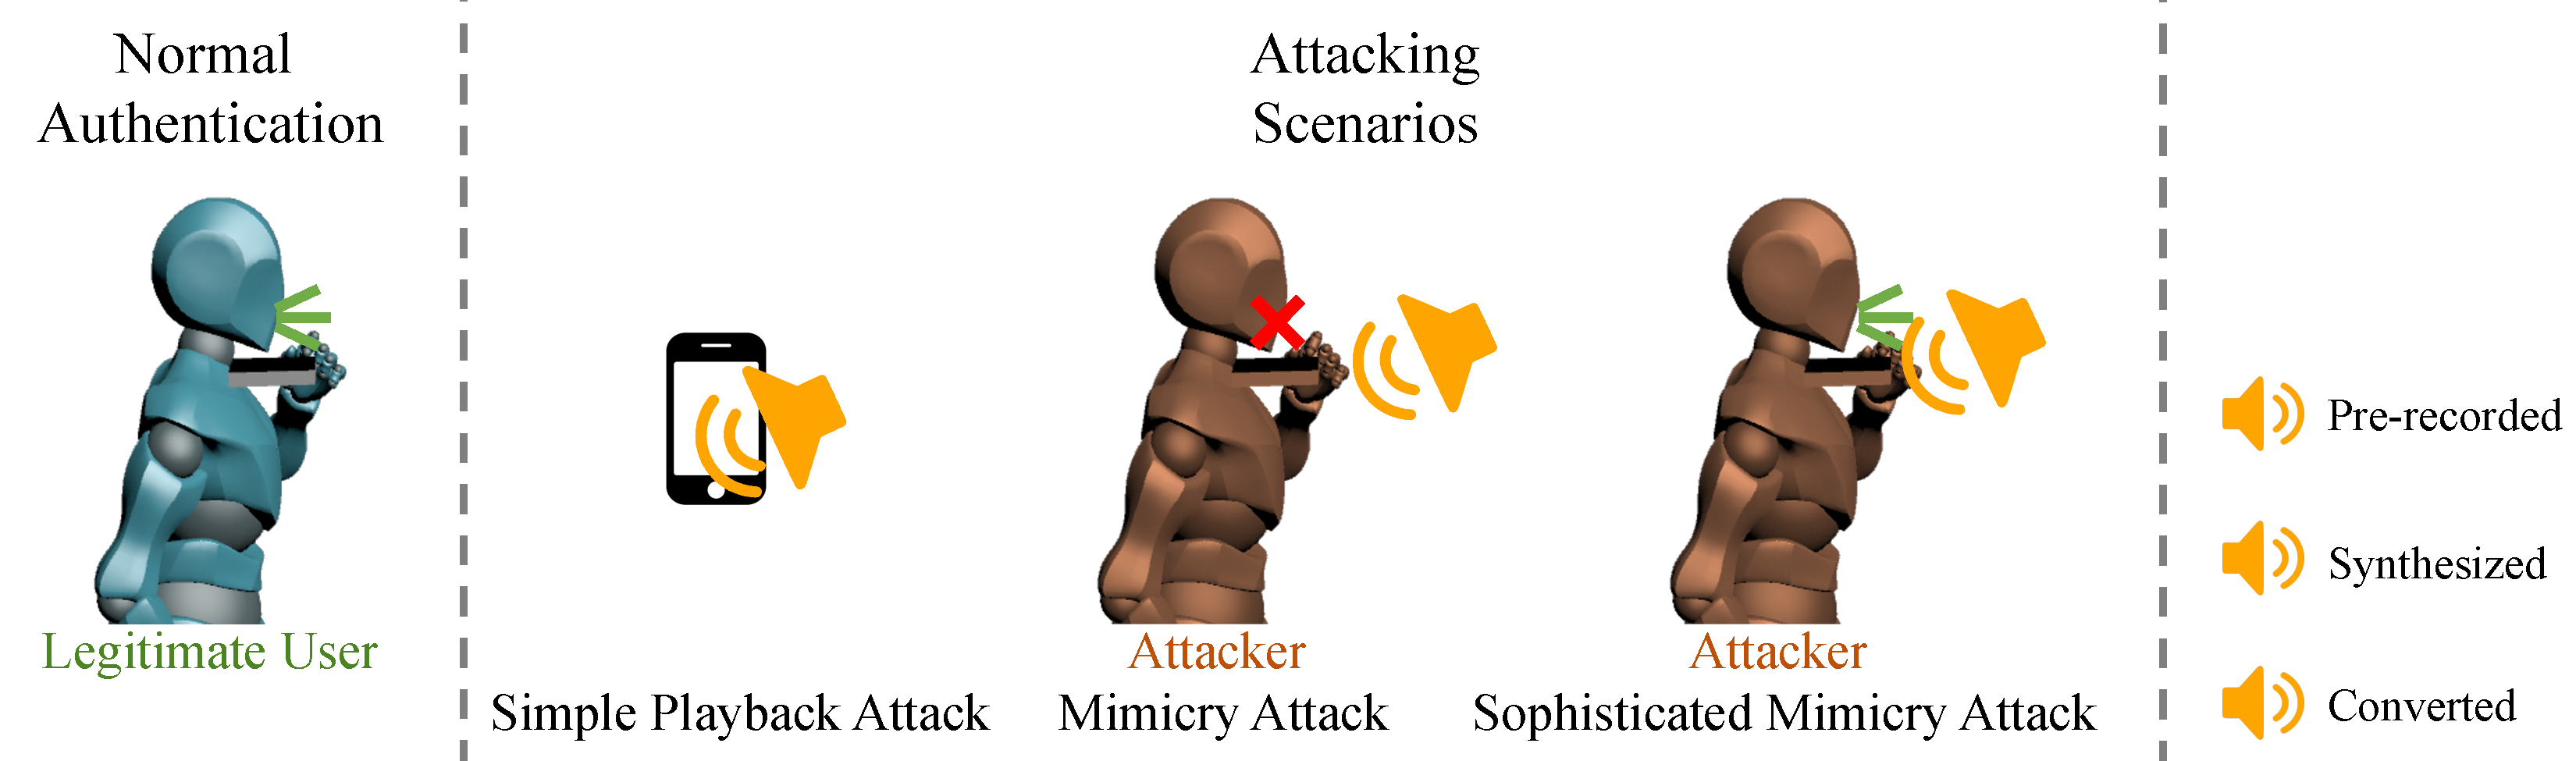
\includegraphics[width=.9\linewidth]{attack}
	\caption[MoVo Attack Model]{Attack Model: There are three types of attack scenarios. To conduct a simple playback attack, the target phone is placed in contact with the electronic speaker. To conduct a mimicry attack, the target phone is placed on the attacker's throat, but the attacker will not speak during the authentication period. As for a sophisticated mimicry attack, the attacker would try to mimic the victim's voice while playing the victim's sounds through electronic speakers. In the two mimicry attacking scenarios, the target phone is also in contact with the electronic speaker. In all three scenarios, the sound played by the electronic speaker could be the pre-recorded sound from the legitimate user, synthesized sound, or converted sound.}
	\label{fig:attack}
\end{figure*}


As mentioned in Section~\ref{sec:spoof}, traditional attacks to voice authentication are impersonation attacks, replay attacks, speech synthesis attacks, and voice conversion attacks. 
%
Real person impersonation attacks can be effectively defended by existing speaker recognition algorithms in general. For the other three, attackers acquire the legitimate user's voice samples either in place or online. The attacker then processes the samples in three ways to perform attacks: replay attack - concatenate voice segments to match the legitimate user's passphrase followed by harmful action or commands; speech synthesis - build speaker model and synthesize passphrase from texts; voice conversion - the attacker says the passphrase, then by spectral mapping and prosody conversion, the signals are manipulated to sound like the legitimate user's. 

If the attacker directly plays the processed sound signals through the speaker, he is conducting the \textit{simple playback attack}, no matter the processed signals are pre-recorded (replay attack), synthesized (speech synthesis), or converted (voice conversion).

A stronger attacker would perform the \textit{mimicry attack}, where the processed signals are still played by electronic speakers, but the attacker also needs to place the smartphone on his throat. In this case, the attacker can observe how the legitimate user passes the authentication\footnote{{\shortname} is a spoof-proof voice authentication system and require users to place the phone on the throat. For best user experience, it can downgrade to a normal voice authentication system and only process microphone data for normal use. Only when the user accesses sensitive information or makes dangerous operation, the spoof-proof mechanism will be invoked and the motion sensor would be in use.} and try to mimic the throat movement of the legitimate user. Note that we do not consider that the attacker uses the built-in speaker of the smartphone to play the processed signal, because if the attacker can control the built-in speaker, he has already hacked the targeted smartphone, which means there is no use to do voice authentication anymore. Therefore, the speaker, shown as yellow icons in Fig.~\ref{fig:attack} must be a different device from the smartphone.


The strongest attack is the \textit{sophisticated mimicry attack}, where the attacker would not only mimic the sound by the electronic device, but also by himself. Compared to the previous case, the attacker would speak the same word along while the electronic speaker is playing. Recall that impersonate the victim's voice using vocal organs is very hard, the attacker should either be professional impersonators or have natural voices similar to the victim's. Such a condition is hard to be met. Therefore, in this thesis, the sophisticated mimicry attacker only controls the timing (starting or pausing when speaking), but not timbre.

Note that we consider two mimicry attacks because these two have different emphasis: the 
mimicry attack makes sure the motion sensor data are affected by the victim's sound, while the sophisticated mimicry attack tries to add ``liveness'' to the motion sensor data. 


\section{System Design}
\label{sec:system}
\subsection{System Overview}
\begin{figure*}[h]
	\centering
	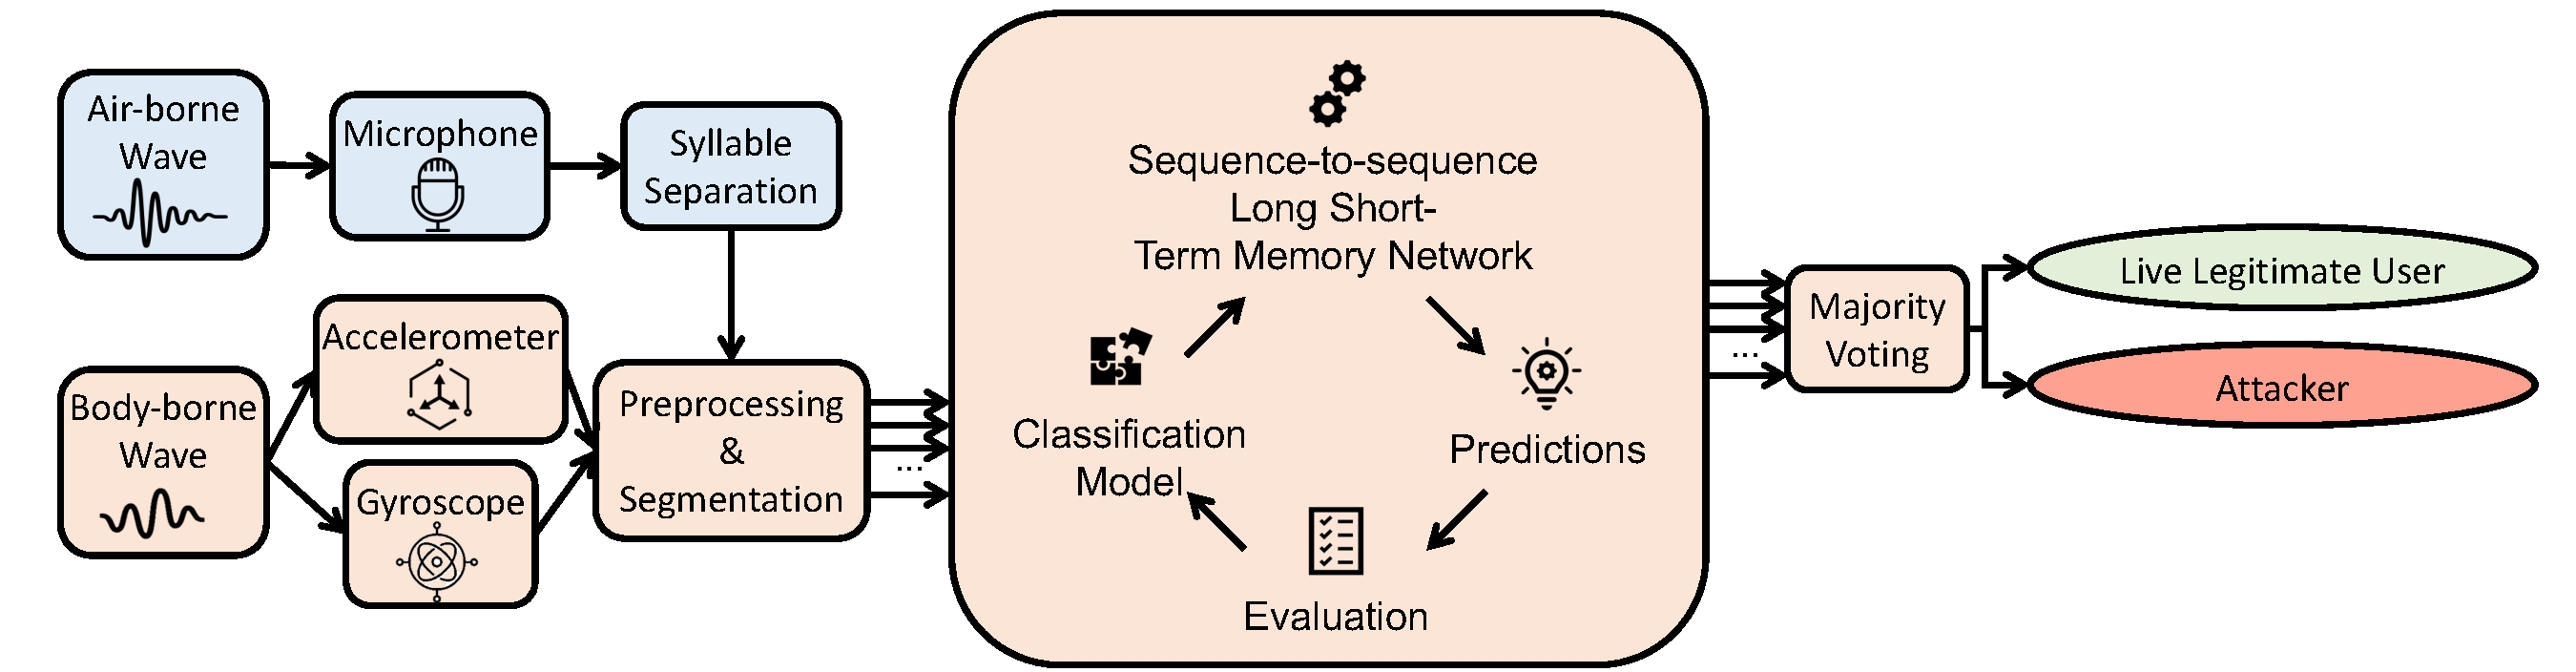
\includegraphics[width=\linewidth]{workflow}
	\caption{The flow of {\shortname}.}
	\label{fig:workflow}
\end{figure*}
\shortname~ currently is a text-dependent voice authentication system. In other words, the speaker recognition algorithm will work on hot-words such as ``Ok Google'', ``Hi Siri'', or ``Alexa''. When a user triggers the voice authentication system, the microphone works normally and the motion sensors measure the modulated and attenuated sound signals at the same time.
%

%TODO
%As shown in Fig.~\ref{fig:workflow}, \shortname~consists of two component groups, one to deal with microphone data (blue shaded components) while the other to deal with motion data (tan shaded components). In detail, the microphone data are used for syllable separation, speech recognition, and speaker recognition. The motion data will first be preprocessed and segmented, then be fed to train a classification model. After a majority voting step, we will match the motion data with hot-words to determine whether the user is a live person or an attacker.
%
Since the hot-words are usually short, less than 2 seconds in our experiment, it is acceptable to process the data together after the whole hot-word is spoken.

We first conduct the syllable separation on speech signals. For example, ``Ok Google'' has 4 syllables in total: O-k-Goo-gle, ``Hi Siri'' has 3, and ``Alexa'' has 3 too. We will, later on, use the detected hot-word beginning and ending time, as well as the syllable nuclei time to segment the accelerometer and gyroscope data.
%
Since the motion data suffer from noises from body movements, heart beats, and breathings, we must preprocess the motion data. We apply a high pass filter to mitigate the noises and increase the target signal. 
%We will also normalize the amplitude and time span of the data, so that the model we built would be user-independent.

We then segment the motion data based on different syllables. We focus on data collected among the syllable nucleus. Because when the sound signal is the maximum, the chance is high that the motion is also the maximum. The maximum motion indicates a higher accuracy of the collected data, which is beneficial for training a more effect and efficient classification model.
%
Another benefit of the segmentation is that segmentation provides the opportunity to do majority voting. For the motion data corresponding to ``Ok, Google'', as long as more than half of the samples are classified to the correct category, we regard the speech and throat movement match each other. This greatly increases the true positive rate of our liveness detection algorithm.

Due to the low sampling rate of motion sensors, the on-body vibration of speech cannot be fully recorded in motion sensors. Finding good representative features is hard. Therefore, we adopt the long short-term memory (LSTM) network, a variant of recurrent neural network (RNN), to help us learn the features on time-domain and classify each segment to each syllable. 

After the majority voting on the classification results on all data samples, \shortname~outputs whether the motion data match the live legitimate user's training model. If yes, a live user is asking the permission; otherwise, an attacker is using a speaker to attack the system. 

%TODO
%Note that we still need to apply speaker recognition algorithm on speech signals to know whether the live user is a legitimate user or an illegal user trying to perform impersonate attack. However, this speaker recognition component is out of the scope of our research topic. For your information, related techniques can be found in~\cite{saquib2010survey,lawson2011survey,wu2015spoofing}.


%When a user triggers the voice assistant, for example, by saying “OK, Google" or “Hey, Siri", our voice assistant extension collects accelerometer data from the wearable component, correlates it with signals collected from microphone and issues the command only
%when there is a match. It is worth noting that the wearable com- ponent of VAuth stays in an idle mode (idle connection and no accelerometer sampling) and only wakes up when it receives a trig- ger from the voice assistant extension

%VAuth consists of two components: (1) a wearable component, responsible for collecting and uploading the accelerometer data, and (2) a voice assistant extension, responsible for authenticat- ing and launching the voice commands. We chose to employ an accelerometer instead of an additional microphone because the accelerometer does not register voice (vibrations) through the air, thus providing a better security guarantee. The first component
%easily incorporates into existing wearable products, such as ear- buds/earphones/headsets, eyeglasses, or necklaces/lockets.
%When a user triggers the voice assistant, for example, by saying “OK, Google" or “Hey, Siri", our voice assistant extension collects accelerometer data from the wearable component, correlates it with signals collected from microphone and issues the command only
%when there is a match. It is worth noting that the wearable com- ponent of VAuth stays in an idle mode (idle connection and no accelerometer sampling) and only wakes up when it receives a trig- ger from the voice assistant extension. After the command finishes, the wearable component goes back to its idle mode. This helps reduce the energy consumption of VAuth’s wearable component by reducing its duty cycle.


%\input{syllable}
\begin{figure}[t]
	\centering
	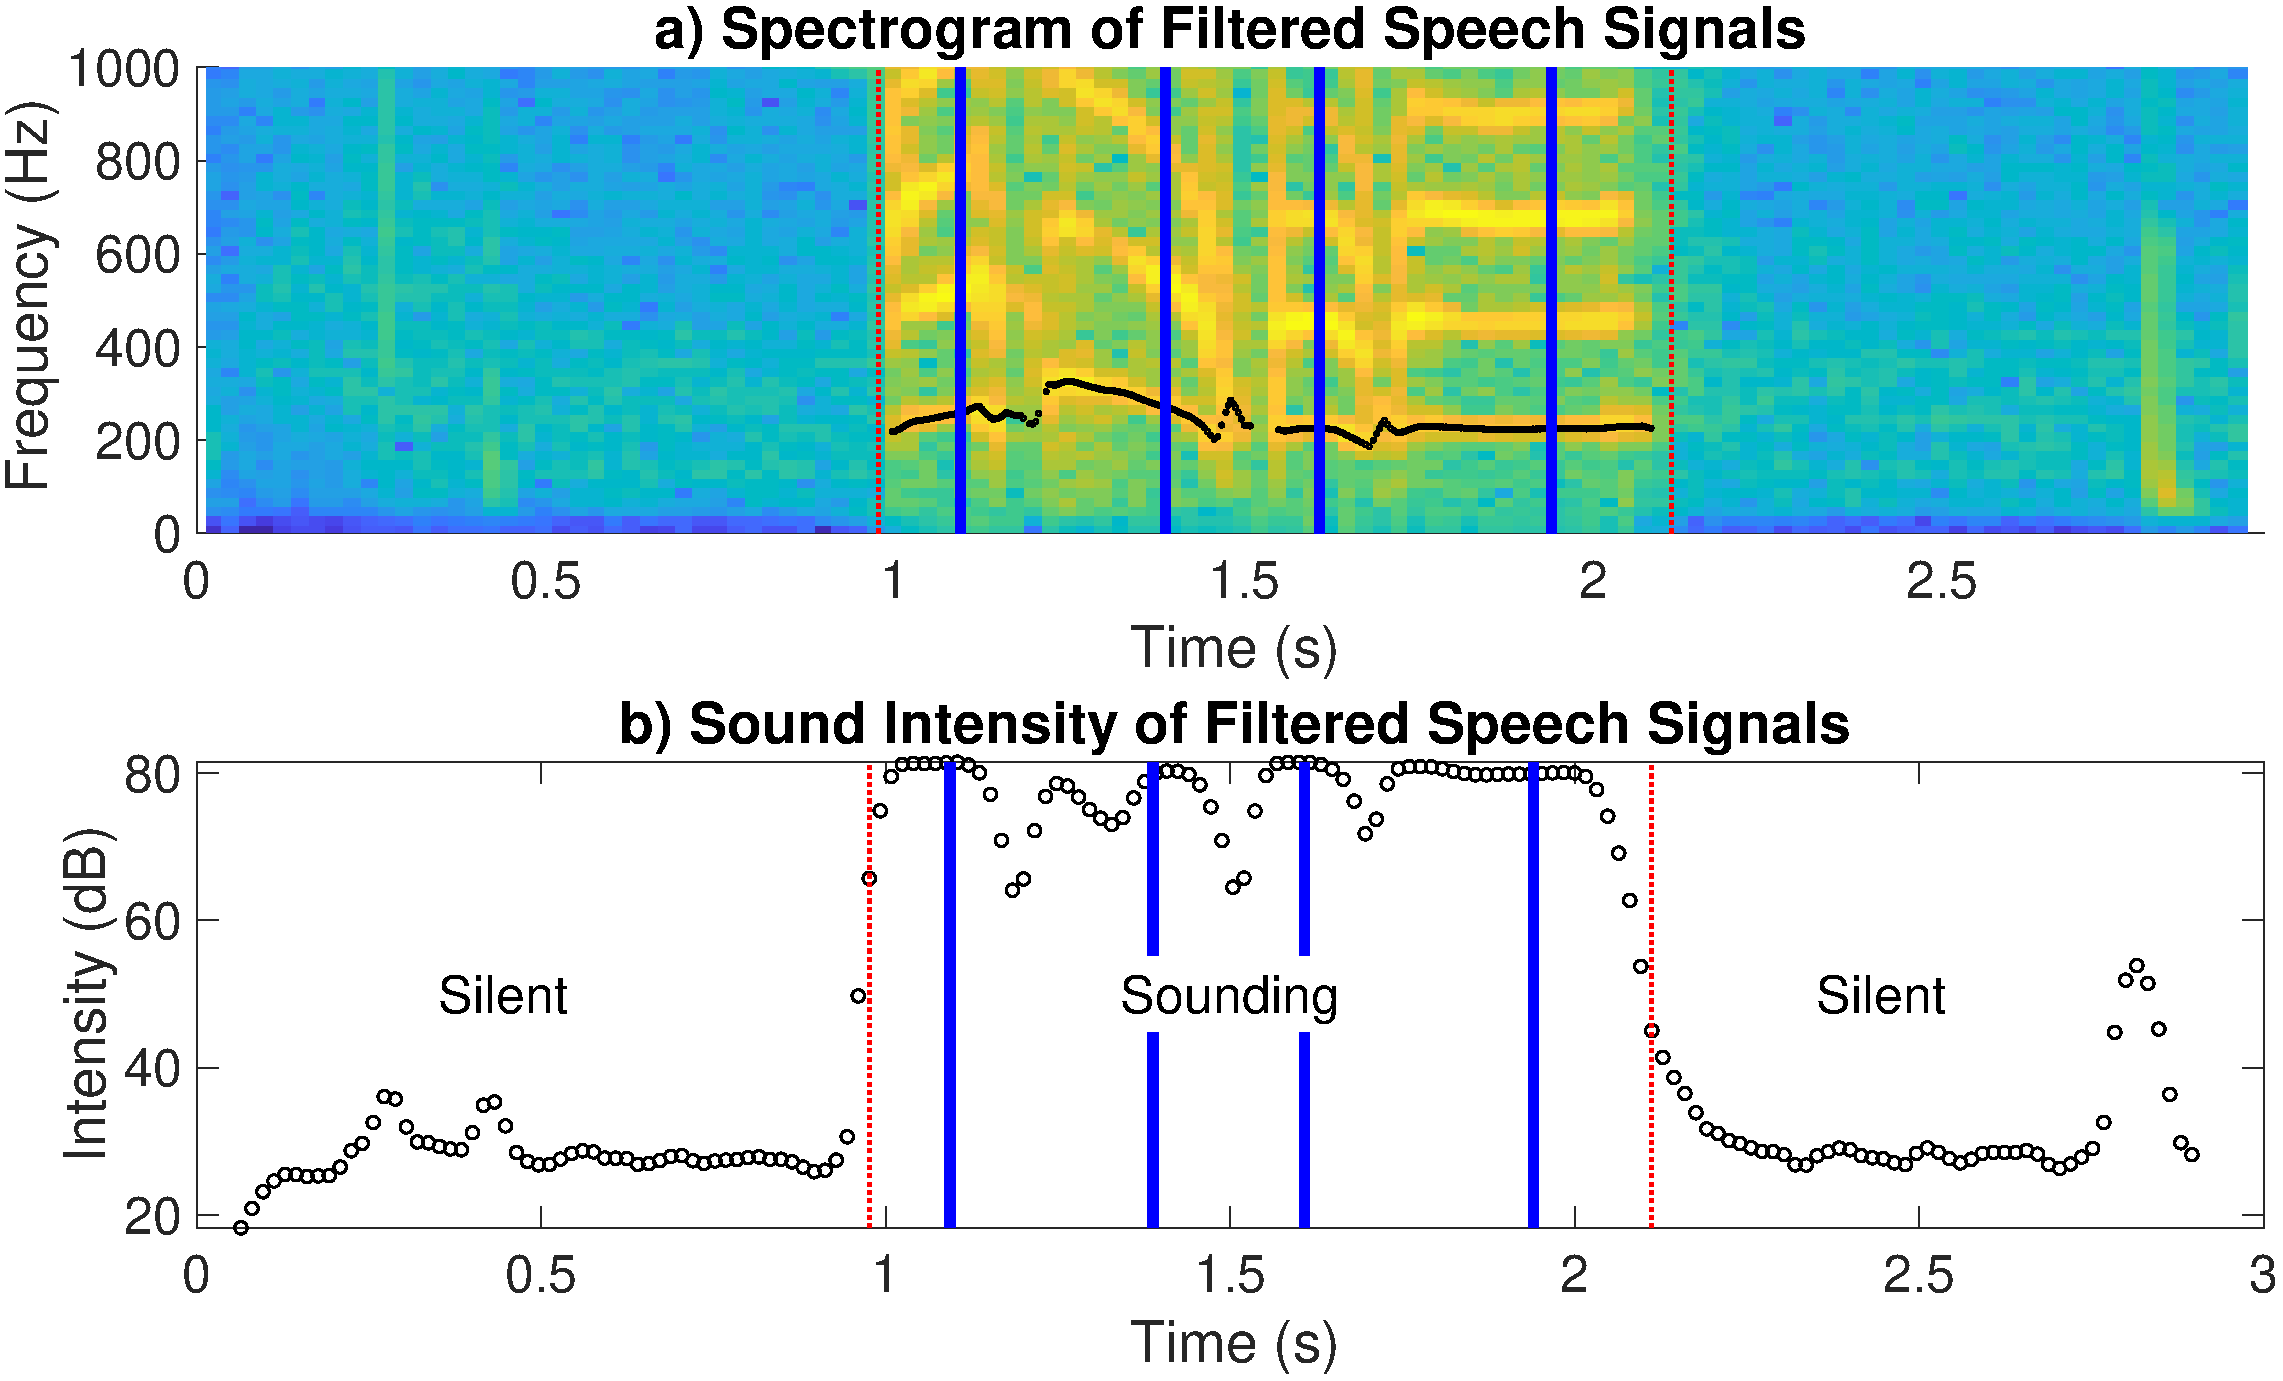
\includegraphics[width=\linewidth]{syllable}
	\caption[Syllable Separation]{Syllable Separation. The original signal is a female user saying ``Ok Google''; then the signal is filtered with a bandpass filter with passing frequency range [50 1000]. The black dots in subfigure a) are the calculated pitches. The vertical red dotted lines indicate the start and end of a sounding period. The blue vertical lines show the calculated time for each syllable nucleus.}
	\label{fig:syllable}
\end{figure}
%TODO  add arrows

\subsection{Syllable Separation}
A syllable is a unit of pronunciation having one vowel sound, with or without surrounding consonants, forming the whole or a part of a word~\cite{onlinesyllable}. The vowel in the middle of a syllable is referred as a \textit{nucleus} in phonetics and phonology. We modify the syllable nuclei detection algorithm proposed by De and Wempe~\cite{de2009praat} and the detailed steps are listed as the following:

%, and implement it in the software program Praat~\cite{onlinepraat}.

\textbf{Step 1}. 
Before conducting the syllable separation, we first apply a $\left[50-1000\right]$ Hz bandpass filter to remove noises so that the frequency range is speech-band limited. We then calculate the intensity and pitch to detect the the syllable nucleus since the vowel within a syllable has higher energy surrounding sounds. 
%



%An Intensity object represents an intensity contour at linearly spaced time points ti = t1 + (i – 1) dt, with values in dB SPL, i.e. dB relative to 2·10-5 Pascal, which is the normative auditory threshold for a 1000-Hz sine wave.
%
%
%The intensity of a sound in air is defined as
%
%%10 log10 { 1 / (T P02) ∫dt x2(t) }
%where x(t) is the sound pressure in units of Pa (Pascal), T is the duration of the sound, and P0 = 2·10-5 Pa is the auditory threshold pressure.
%In what follows, we describe the sequence of actions that the script completes to find syllable nuclei using intensity (dB) and voicedness. 
%We use intensity first to be able to find peaks in the energy contour, since a vowel within a syllable (the syllable nucleus) has higher energy than do surrounding sounds (described in Steps 1 and 2, below). 
%
%With this procedure, we delete multiple peaks within one syllable (described in Step 3, below). 

%Finally, we use voicedness to exclude peaks that are unvoiced, which is required to delete surrounding voiceless consonants that have high intensity (described in Step 4, below). 
%
%Before the script is run, sound files that are quite noisy should be filtered so that the frequency range is speech-band limited.
%


\textbf{Step 2}. 
The intensity of a sound in air is the sound pressure level relative to $2*10^{-5}$ Pascal, which is the normative auditory threshold for a 1000-Hz sine wave. We calculate the intensity contour by squaring all values in the sound, then convolved with a Kaiser window.  To guarantee that a periodic signal is analyzed as having a pitch-synchronous intensity ripple not greater than 0.00001 dB, we set the length of the Kaiser window to be 64 ms and the sidelobe height to be -190 dB. In this way, we are able to find peaks in the energy contour

%
% (Kaiser-20; sidelobes below -190 dB). The effective duration of this analysis window is 3.2 / (minimum\_pitch), which will guarantee that a periodic signal is analysed as having a pitch-synchronous intensity ripple not greater than 0.00001 dB.

%
%
%We extract the intensity, with the parameter
%“minimum pitch” set to 50 Hz, using autocorrelation. With
%this parameter setting, we extract intensity smoothed over
%a time window of 64 msec, with 16-msec time steps.

\textbf{Step 3}. We consider all peaks above a certain threshold
in intensity to be potential syllables. We set the threshold
to 20dB below the maximum intensity measured over the
total sound file.

\textbf{Step 4}. We then use the intensity contour to make sure that the intensity between the current peak and the preceding peak is sufficiently low.  We consider only a peak with a preceding dip of at least 2 dB with respect to the current peak as a potential syllable. In this way, we also delete multiple peaks within one syllable.

\textbf{Step 5}.
We use the algorithm proposed by Boersma ~\{boersma1993accurate\} to calculate the pitch (fundamental frequency) contour of audio data. The window size is set to be  100 ms with 20 ms time steps. We then exclude all peaks that are unvoiced. The remaining peaks are considered syllable nuclei and will be used to segment motion data.

Fig.~\ref{fig:syllable} shows the pitch contour in subfigure a) and the intensity countour in subfigure b). The resulting appearance times of syllable nuclei are marked using blue vertical lines.





%\input{preprocess}
\subsection{Preprocessing and Segmentation}
\begin{figure*}[h]
	\centering
	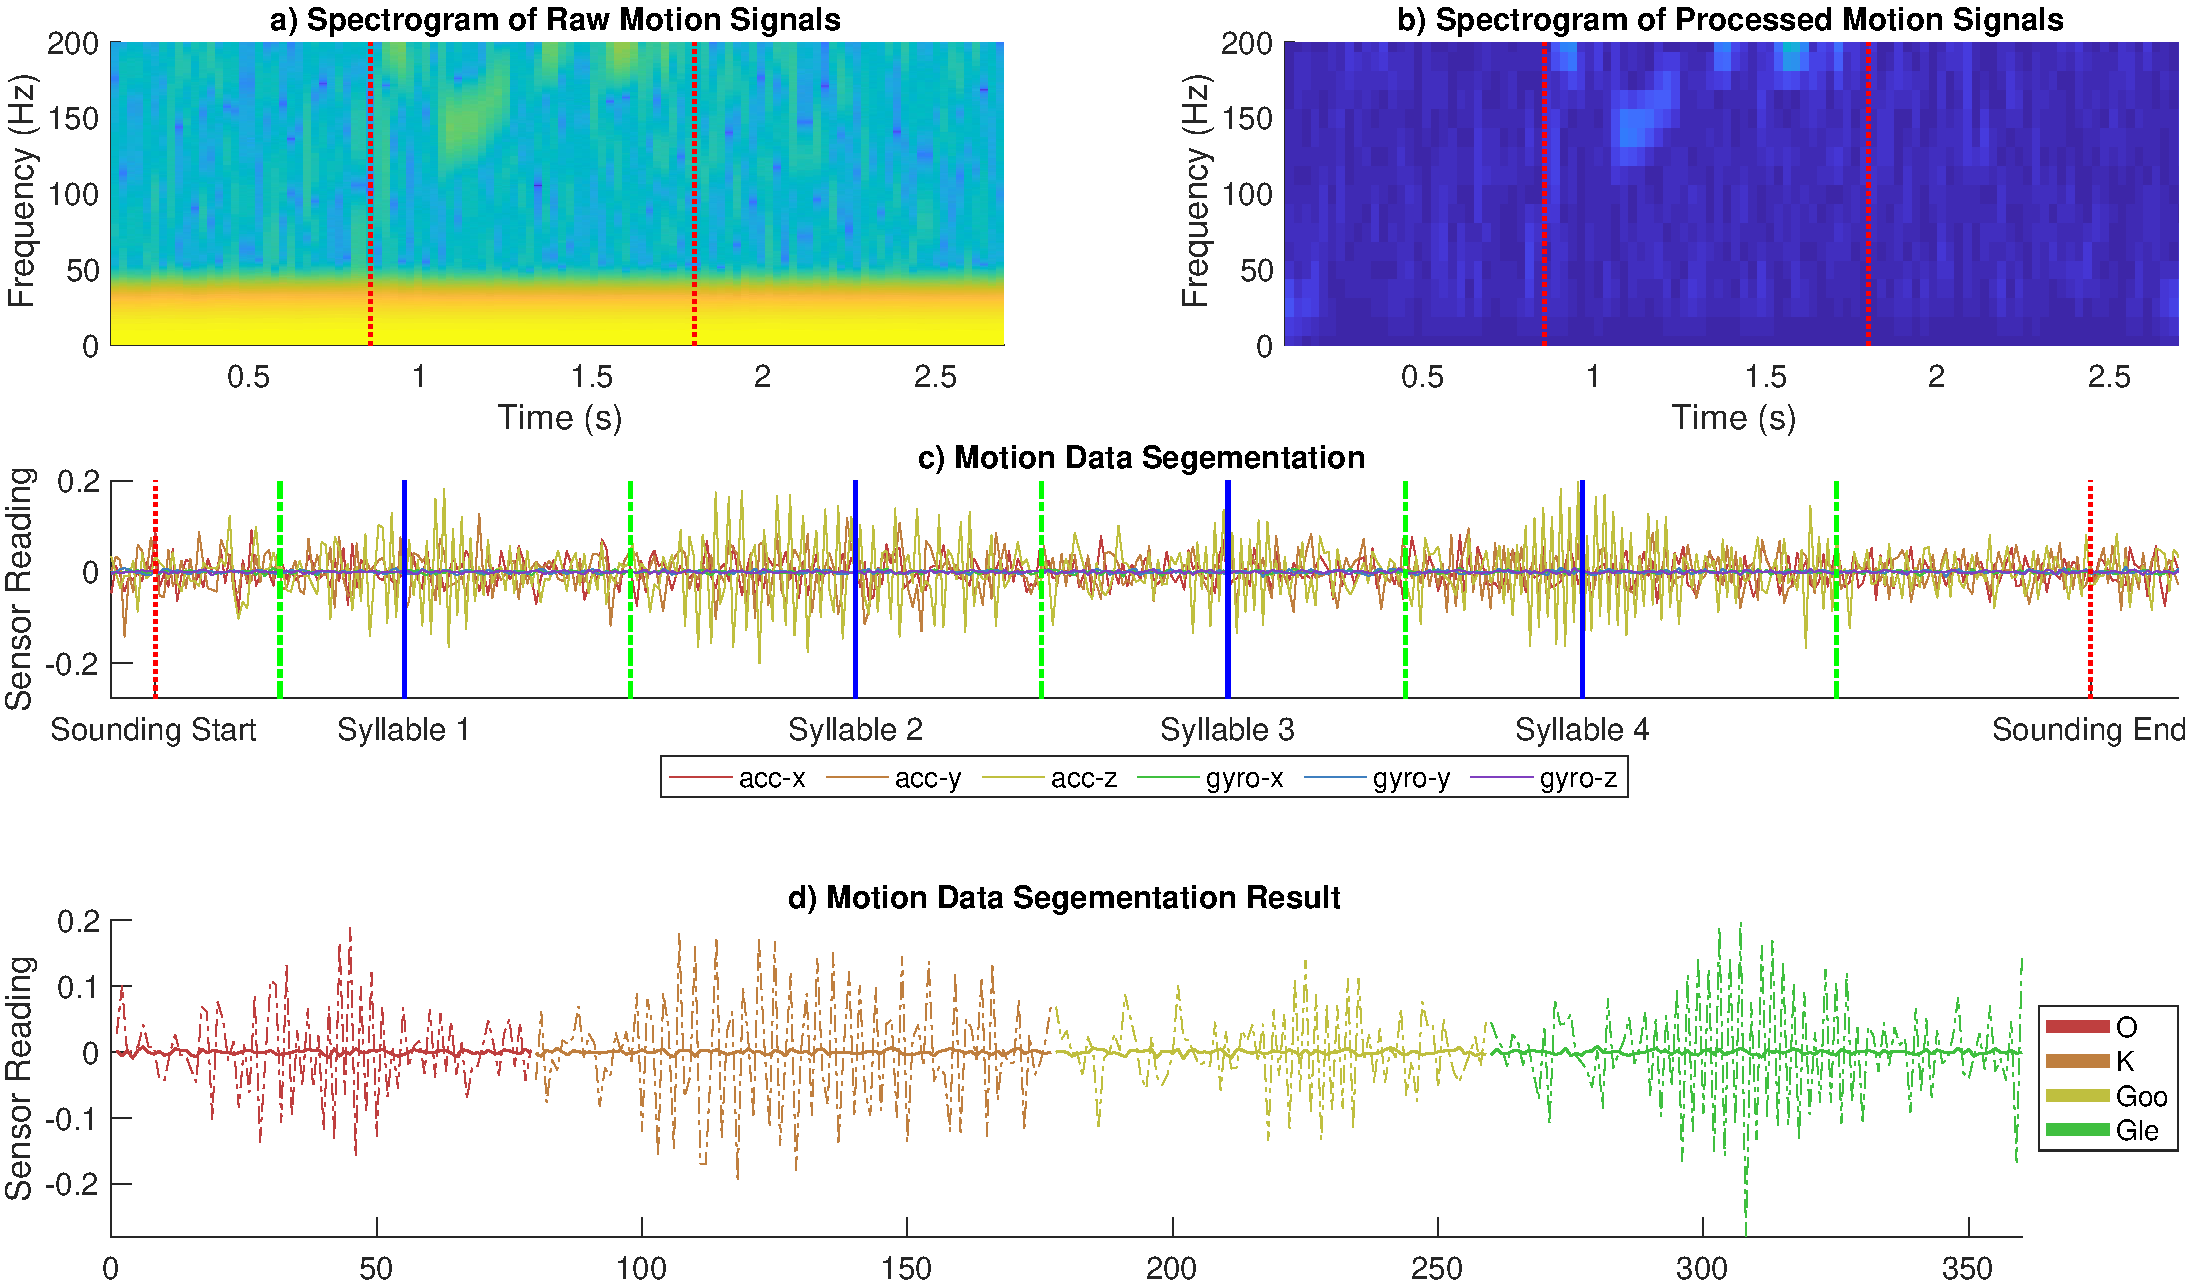
\includegraphics[width=\linewidth]{preprocess}
	\caption{Preprocessing and Segmentation. }
	\label{fig:preprocess}
\end{figure*}
The motion data is impeded by low sampling rate, low target movement, and large interfere noises. To overcome such a problem, we must preprocess the motion data. We apply a high pass filter to mitigate the noise and increase the signal-to-noise ratio. The cutoff frequency is set to be 100 Hz, since noises such as breathing or walking or other human movements can not create signals as high as 100 Hz. As shown in Fig.~\ref{fig:preprocess}, after applying a high pass filter, the motion data in Fig.~\ref{fig:preprocess}b is much more cleaner than the original data in Fig.~\ref{fig:preprocess}a. 

We then use the syllable nuclei calculated in previous section to segment the motion data. As shown in Fig.~\ref{fig:preprocess}c, we first calculate the half time points (green lines) from sounding start time (red line), syllable times (blue lines), and sound end time (red line). Then we extract each segmentation from two adjacent half time points (green lines). Note that if the time duration between two adjacent half time points is large than 100 samples,  we will only keep the middle 100-samples data and discard the data at the beginning area and the end area. This is because the data far from syllable nuclei are not as reliable as data around syllable nuclei. Keeping those unreliable data does no good to the classification model.
%
Lastly, concatenating reliable data around syllable nuclei together gives the final processed data. One example of the resulting segmentation is illustrated in Fig.~\ref{fig:preprocess}d. Note that Fig.~\ref{fig:preprocess}c shows motion data of all six dimensions, while Fig.~\ref{fig:preprocess}d only shows two of them: the data of the solid line is  from the gyroscope and the data of the dashed line is from the accelerometer.

Note that we do not consider the synchronization problem between the microphone and the motion sensors. This is because the sampling rate of motion sensors is set to be 400Hz, which means that an error with just one sample represents 1/400=0.0025 s. Within such a period of time, the sound travels about 343 m/s * 0.0025 s $\approx$ 0.85 m  in air, which is much longer than the distance between the voice source and the microphone. In other words, due to the low sampling rate of motion sensors, the true lag between microphone reading and motion reading always falls in one sample period, which makes the synchronization procedure unnecessary. 

%TODO remove subfigure


%\input{lstm}
\subsection{The LSTM Network}
%TODO RNN
After the preprocessing and segmentation of the motion data, we use the data to establish a sequence-to-sequence Long Short-Term Memory (LSTM) network model. LSTM was first proposed by Sepp Hochreiter and J{\"u}rgen Schmidhuber in 1997 ~\cite{hochreiter1997long}. It is a special variant of  Recurrent Neural Networks (RNN), and is widely used in learning, processing, and classifying sequential data because of 
its great property of selectively remembering patterns for long durations of time. Over the years, there have also been many variants of LSTM networks. However, based on a study in 2017, none of the variants can improve upon the standard LSTM architecture significantly~\cite{greff2017lstm}. Therefore, we still choose to implement the standard LSTM network in this work.

%Short-Term duplicate 
%change figure font display
%\begin{figure}[h]
%	\centering
%	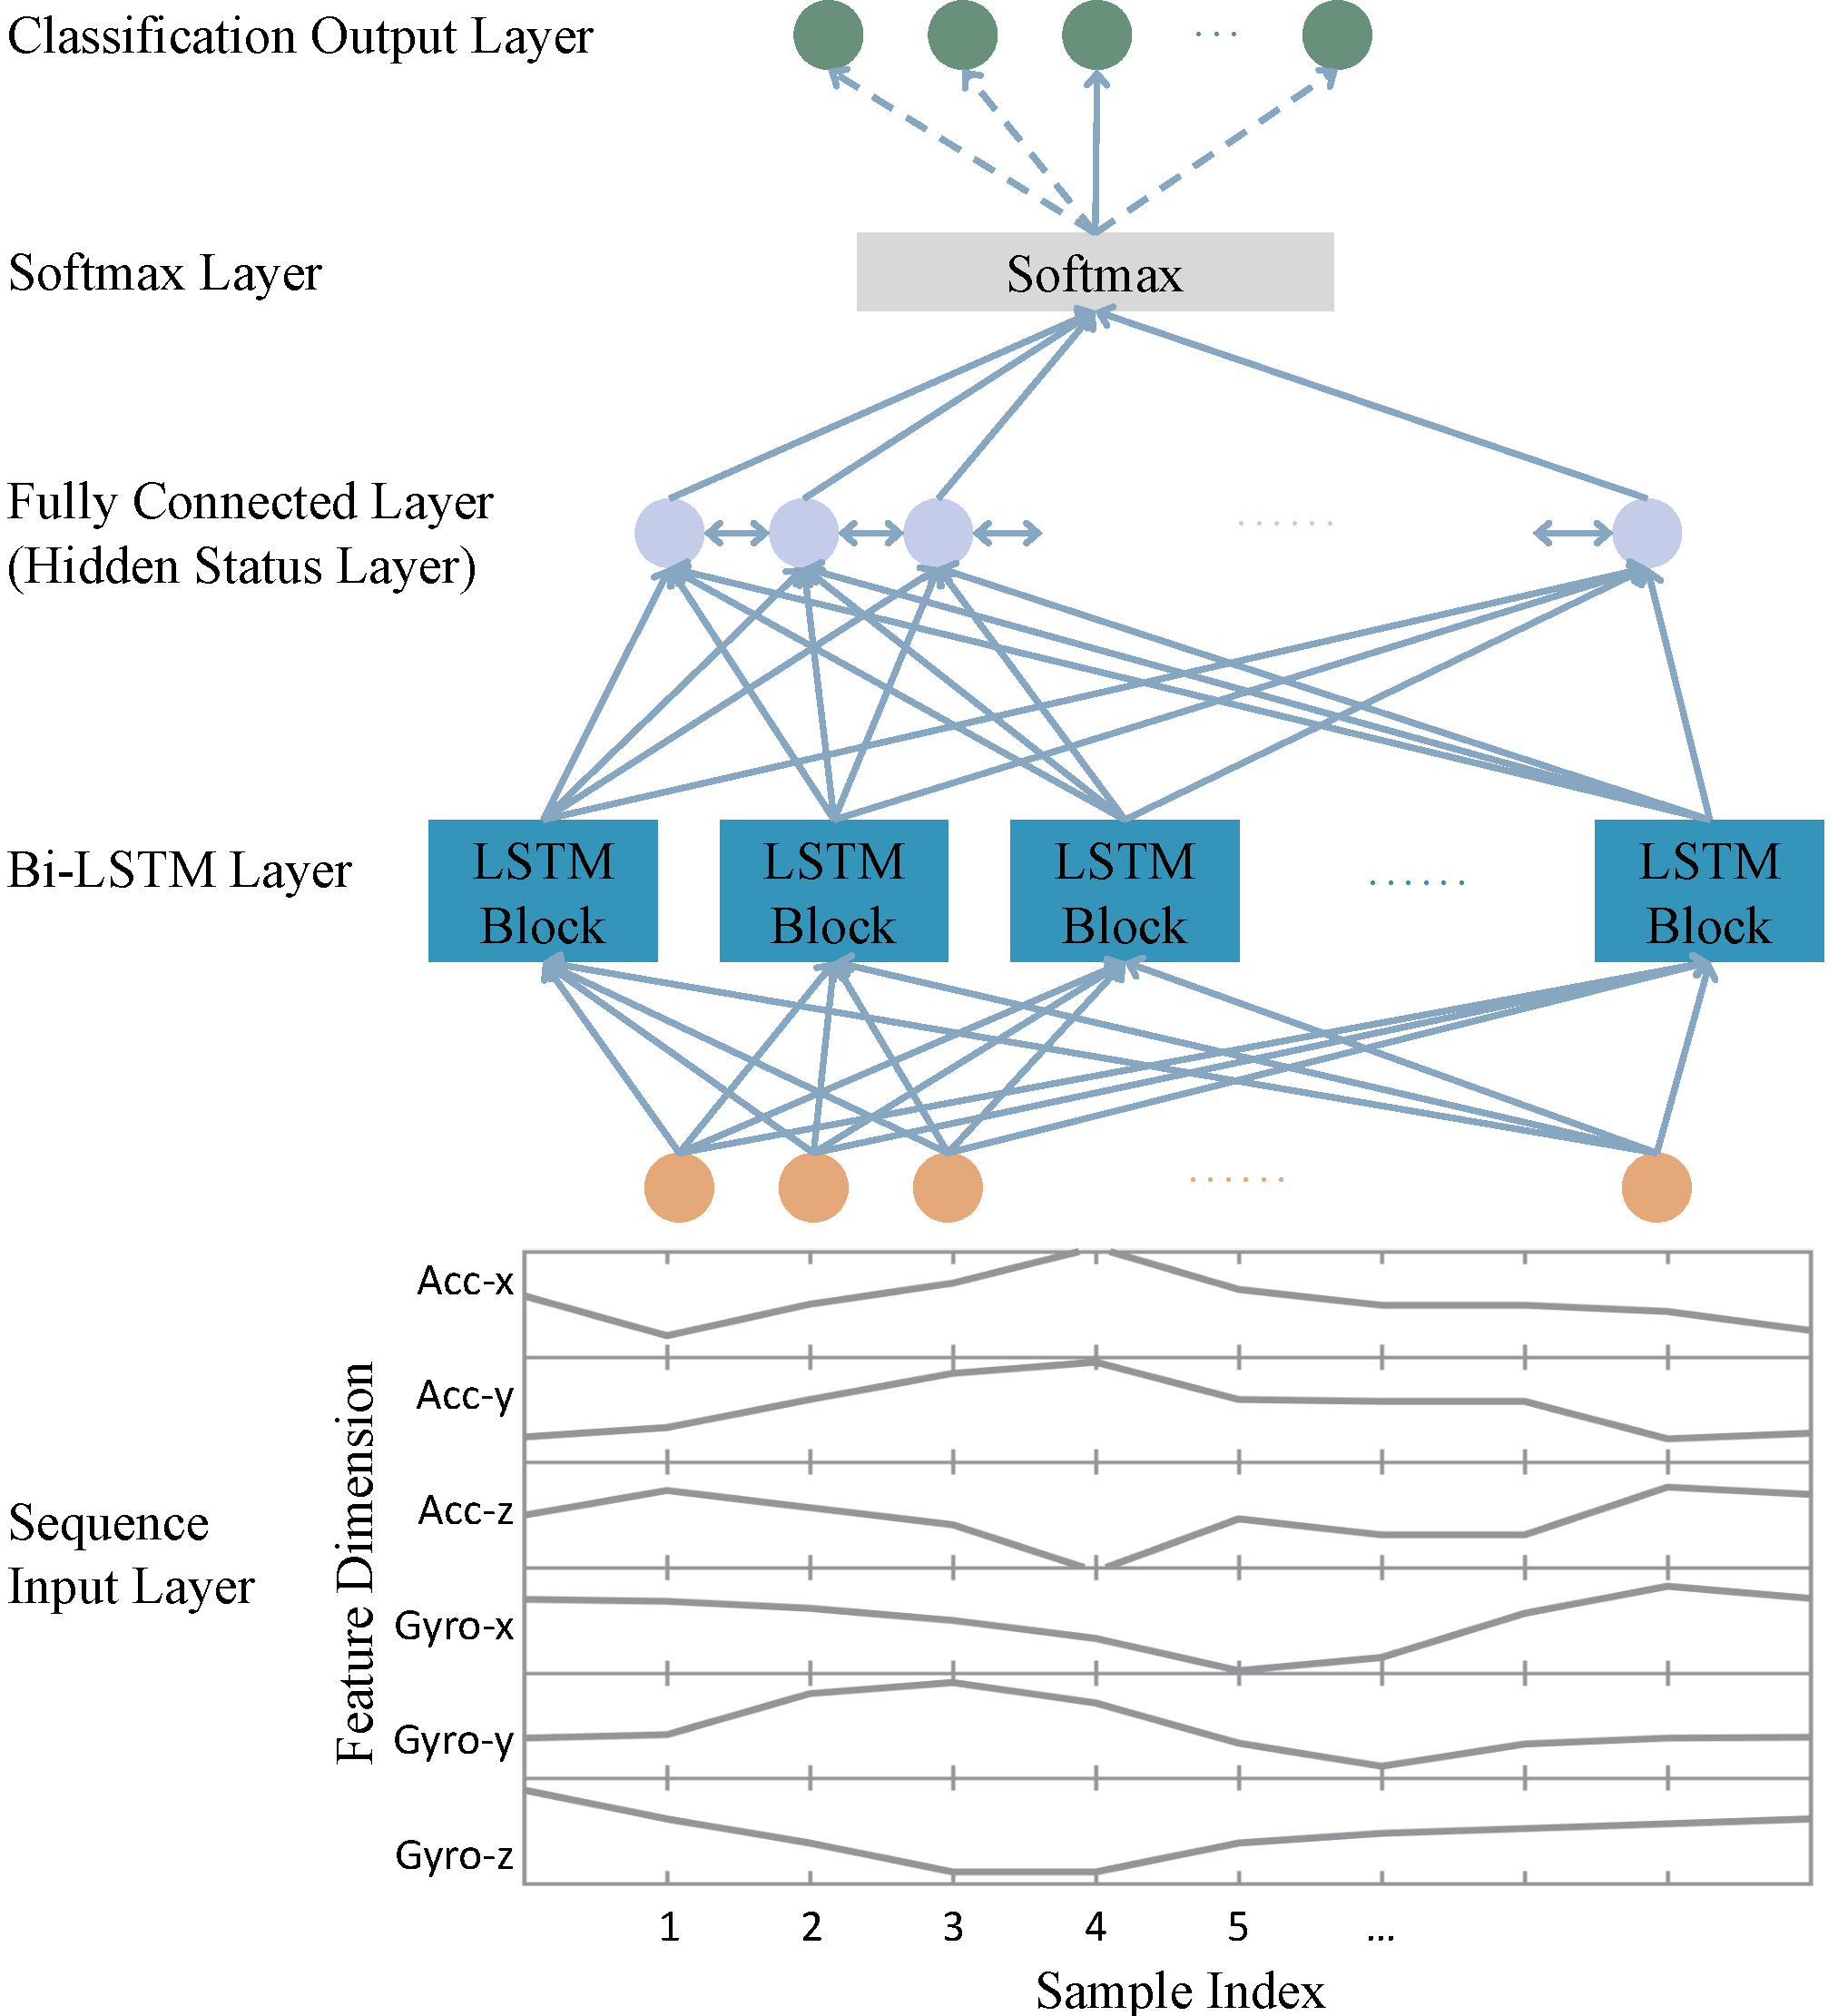
\includegraphics[width=.9\linewidth]{rnn}
%	\caption{The sequence-to-sequence Long Short-Term Memory network (LSTM network) used in \shortname.}
%	\label{fig:rnn}
%\end{figure}

Our sequence-to-sequence LSTM has five layers in total and it is able to make different predictions for each individual time step of the input data. In the sequence input layer, the input data have 6 feature dimensions, which consists of 3 accelerometer dimensions and 3 gyroscope dimensions. Then we establish an LSTM layer formed by LSTM blocks, where each block publish its cell state to the next LSTM block. The output of the LSTM layer is the fully connecte hidden status layer. We set the total number of hidden units to be 100, then feed the hidden status to a softmax function and output the classification of each time step of input data.


%\input{majority}
\section{Majority Voting}

%\begin{figure}[h]
%	\centering
%	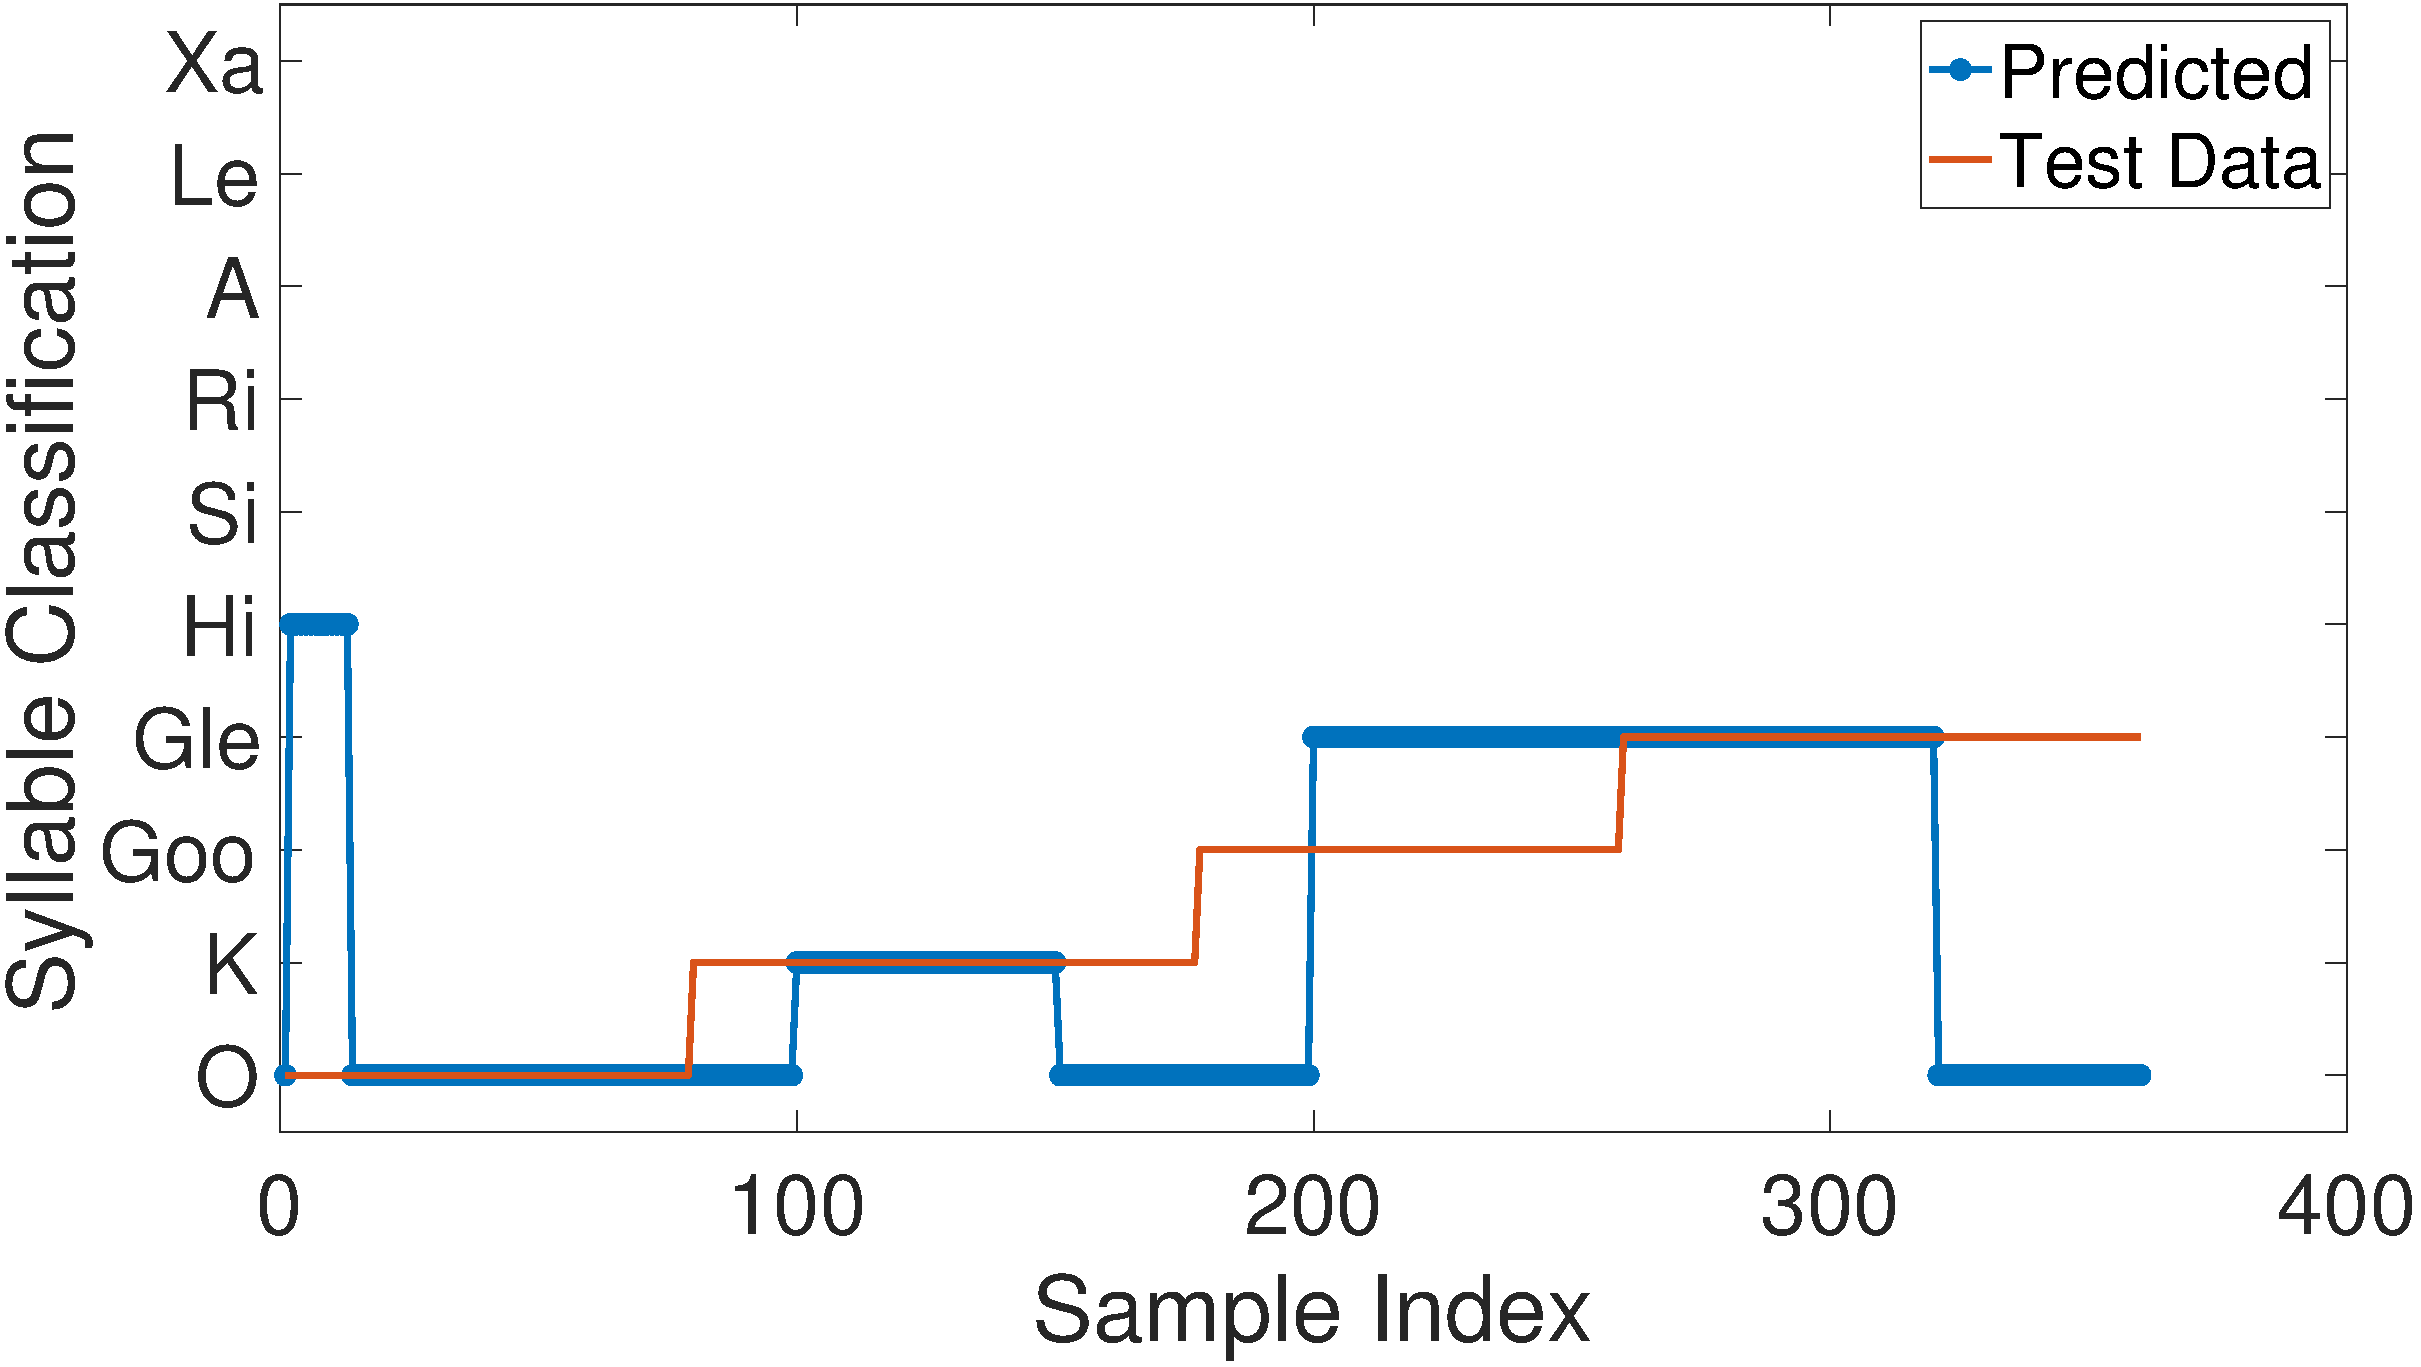
\includegraphics[width=.6\linewidth]{majority}
%	
%\end{figure}

\begin{figure}
	\centering
		\centering
		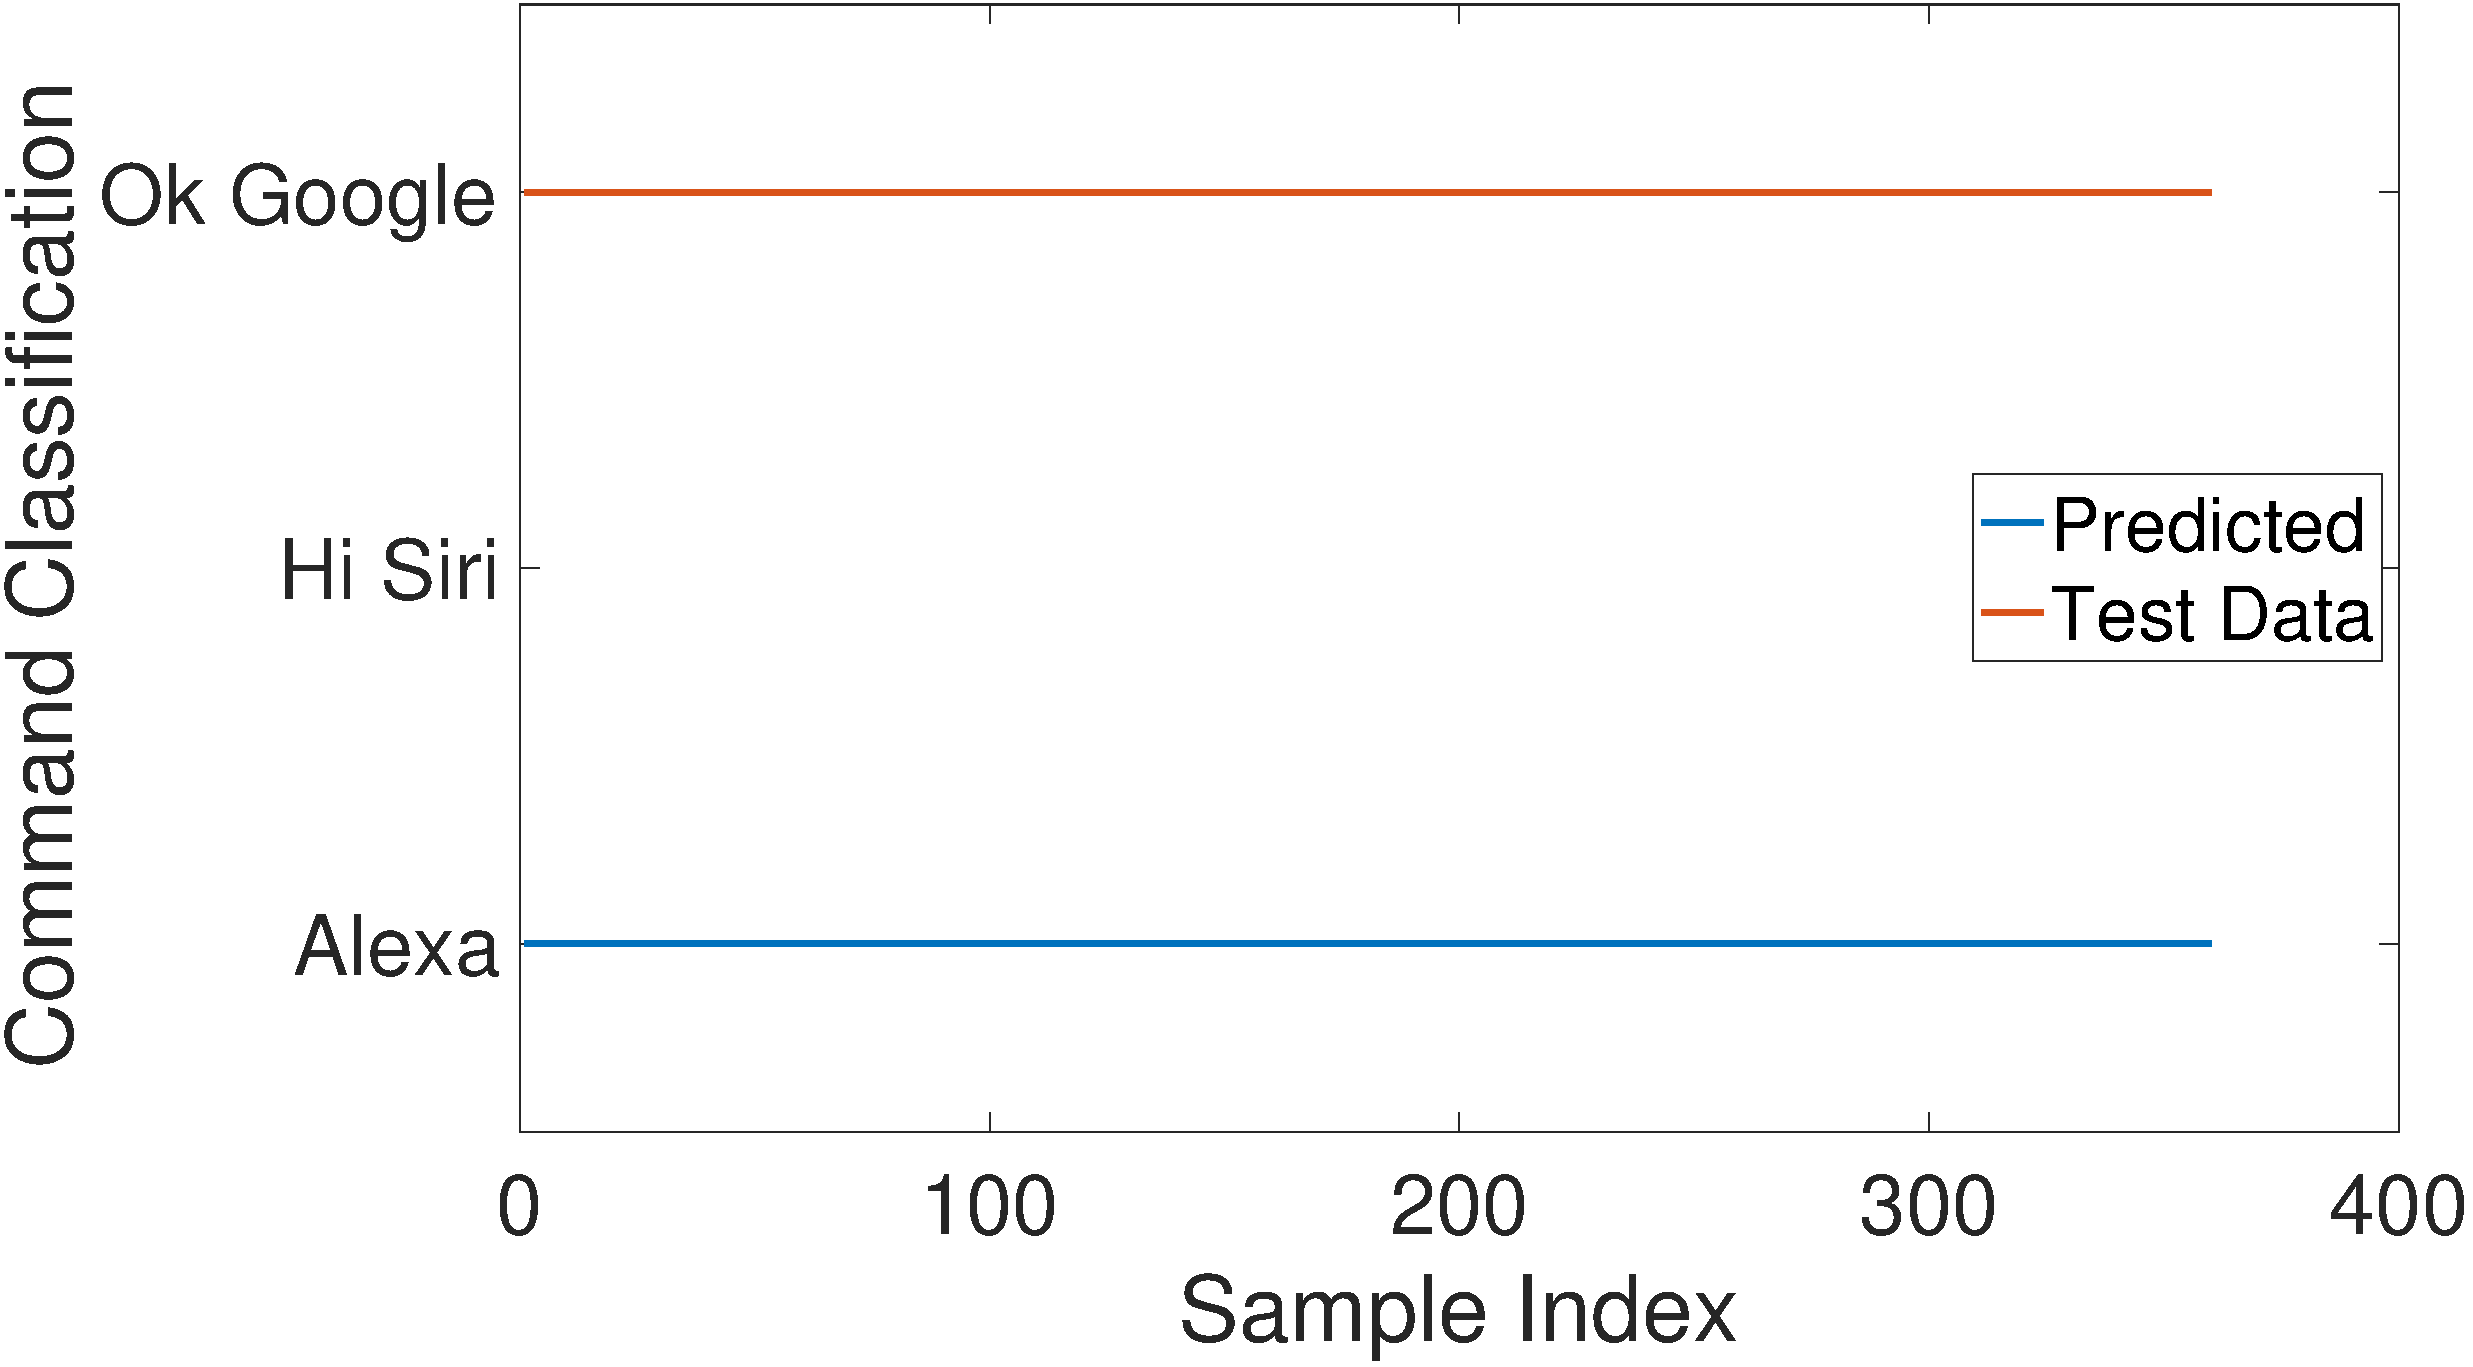
\includegraphics[width=.5\linewidth]{nonmajority}
		\caption{Classification result without syllable separation and majority voting: Falsely classifying an `Ok Google' sample to `Hi Siri'.}
		\label{fig:nonmajority}
\end{figure}
\begin{figure}
	
		\centering
		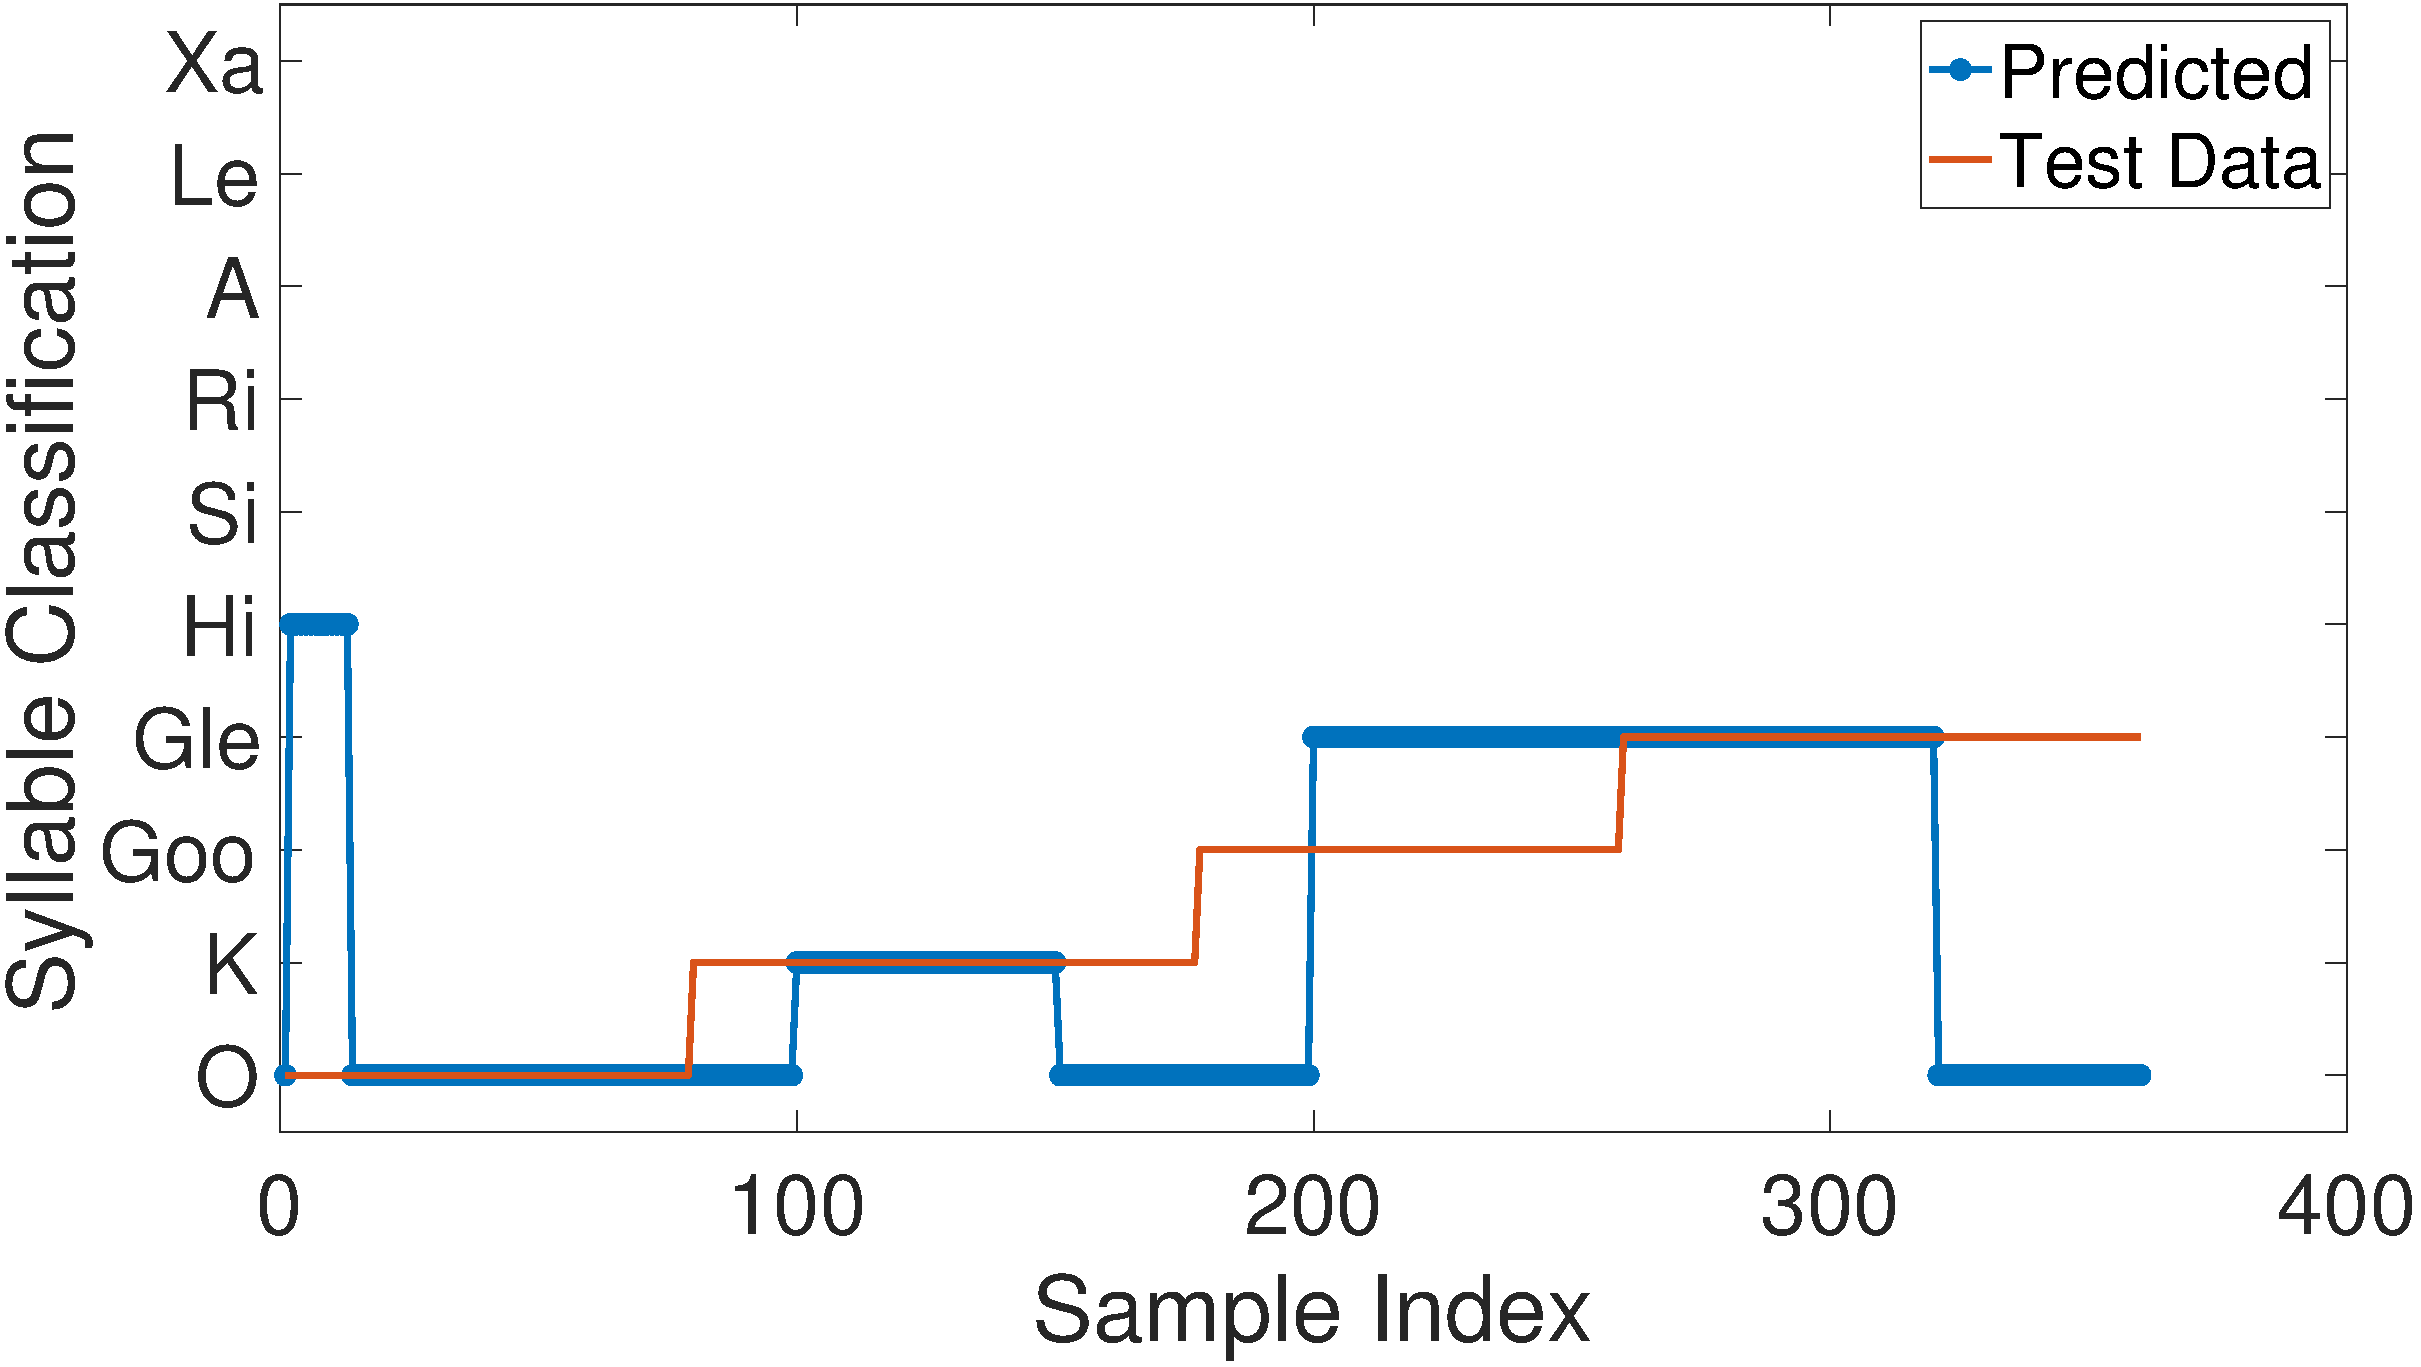
\includegraphics[width=.5\linewidth]{majority}
		\caption[Classification Result]{Classification result from the sequence-to-sequence LSTM network. Although many parts of the classification is incorrect, with majority voting, the final classification is the correct `Ok Google'. }
		\label{fig:majority}

\end{figure}


Since we are using the sequence-to-sequence LSTM network, an example classification result is shown in Fig.~\ref{fig:majority}. Though the ground truth of the test data is O-K-Goo-Gle, the predicted result is O-Hi-O-K-O-Gle-O. However, with a majority voting algorithm, as long as half of the sample falls in category `O', `K', `Goo' and `Gle', we will regard the whole input data as in category `Ok Google'. The principle behind this majority voting is the consistency of the throat movement when speaking different syllables of one single command. In addition, since the syllable segmentation algorithm is heuristic, its uncertainty in separating syllables also increases the demand of adopting majority voting to compensate for the uncertainty.
%TODO
In all, adopting syllable separation and majority voting can greatly increase the true positive rate of {\shortname}.  

%compared to classification without syllable separation and majority voting, as an example shown in Fig.~\ref{fig:nonmajority}, 


\textbf{Remark.} In our experiment, we only train our model with 10 syllables since our system is designed as a text-dependent voice authentication system. However, with larger training database, we can build a model with more syllables, and extend our system to work for text-independent systems. According to~\cite{onlinelist}, 322 syllables can form 5000 most frequent English words. With such extension, {\shortname} can also become a continuous voice authentication system.


%\subsection{Bi-LSTM Learing}
%
%The last stage is to use the reconstructed data to establish a Bi-directional Long Short-Term Memory (Bi-LSTM) network model, which will be used for classifying the input data later on.
%
%LSTM was first proposed by Sepp Hochreiter and J{\"u}rgen Schmidhuber in 1997 ~\cite{hochreiter1997long}. It is a special variant of  Recurrent Neural Networks (RNN), and is widely used in learning, processing, and classifying \textit{sequential } data because of 
%its great property of selectively remembering patterns for long durations of time. 
%
%
%
%
%Over the years, there have also been many variants of LSTM networks. However, based on a study in 2017, none of the variants can improve upon the standard LSTM architecture significantly~\cite{greff2017lstm}. Therefore, we still choose to implement the standard LSTM network in this work except for the bi-directional calculation. The original unidirectional LSTM network only preserves information from the inputs seen at the past. Bi-LSTM network, on the contrary, preserves information both from the past and the future. 
%
%%Short-Term duplicate 
%%change figure font display
%
%
%As shown in Fig.~\ref{fig:rnn}, our Bi-LSTM  network has five layers in total. In the sequence input layer, the input data have 6 feature dimensions, which consists of 3 accelerometer dimensions and 3 gyroscope dimensions. Then we establish an LSTM layer formed by LSTM blocks, where each block publishes its cell state to the next LSTM block. The output of the LSTM layer is sent to the fully connected hidden status layer. We set the total number of hidden units to be 100, and each hidden unit has two hidden states, one from the past and the other from the future. Then we feed the combined hidden status to a softmax function and output the classification of the input data.

\section{Implementation and Evaluation}


\textbf{Phones and Placements.} We use Huawei Nexus 6P Android smartphone to collect user data. Since we mainly use the microphone data to detect the syllable nuclei time, we do not require a high sampling frequency of audio data. Indeed, we only record the data at 8000 Hz (telephone quality). For the motion data, however, the sample frequency is the higher the better. The Nexus 6P is manufactured in 2015, but we have updated its operating system to Android Orea (API level 26), which is released in 2017. By calling the \texttt{getMinDelay()} function, we found the minimum delay allowed between two motion sensor events is 2500 microsecond, which is a sample frequency of 400 Hz. Therefore, we use 400 Hz for both gyroscope and accelerometer. As shown in Fig.~\ref{fig:use}, a smartphone user places his device to his throat tightly so that conductive vibrations can be measured. The data collection app is shown in ~\ref{fig:defendappa}.

\begin{figure}[H]
	\centering
	\begin{minipage}{.3\linewidth}
		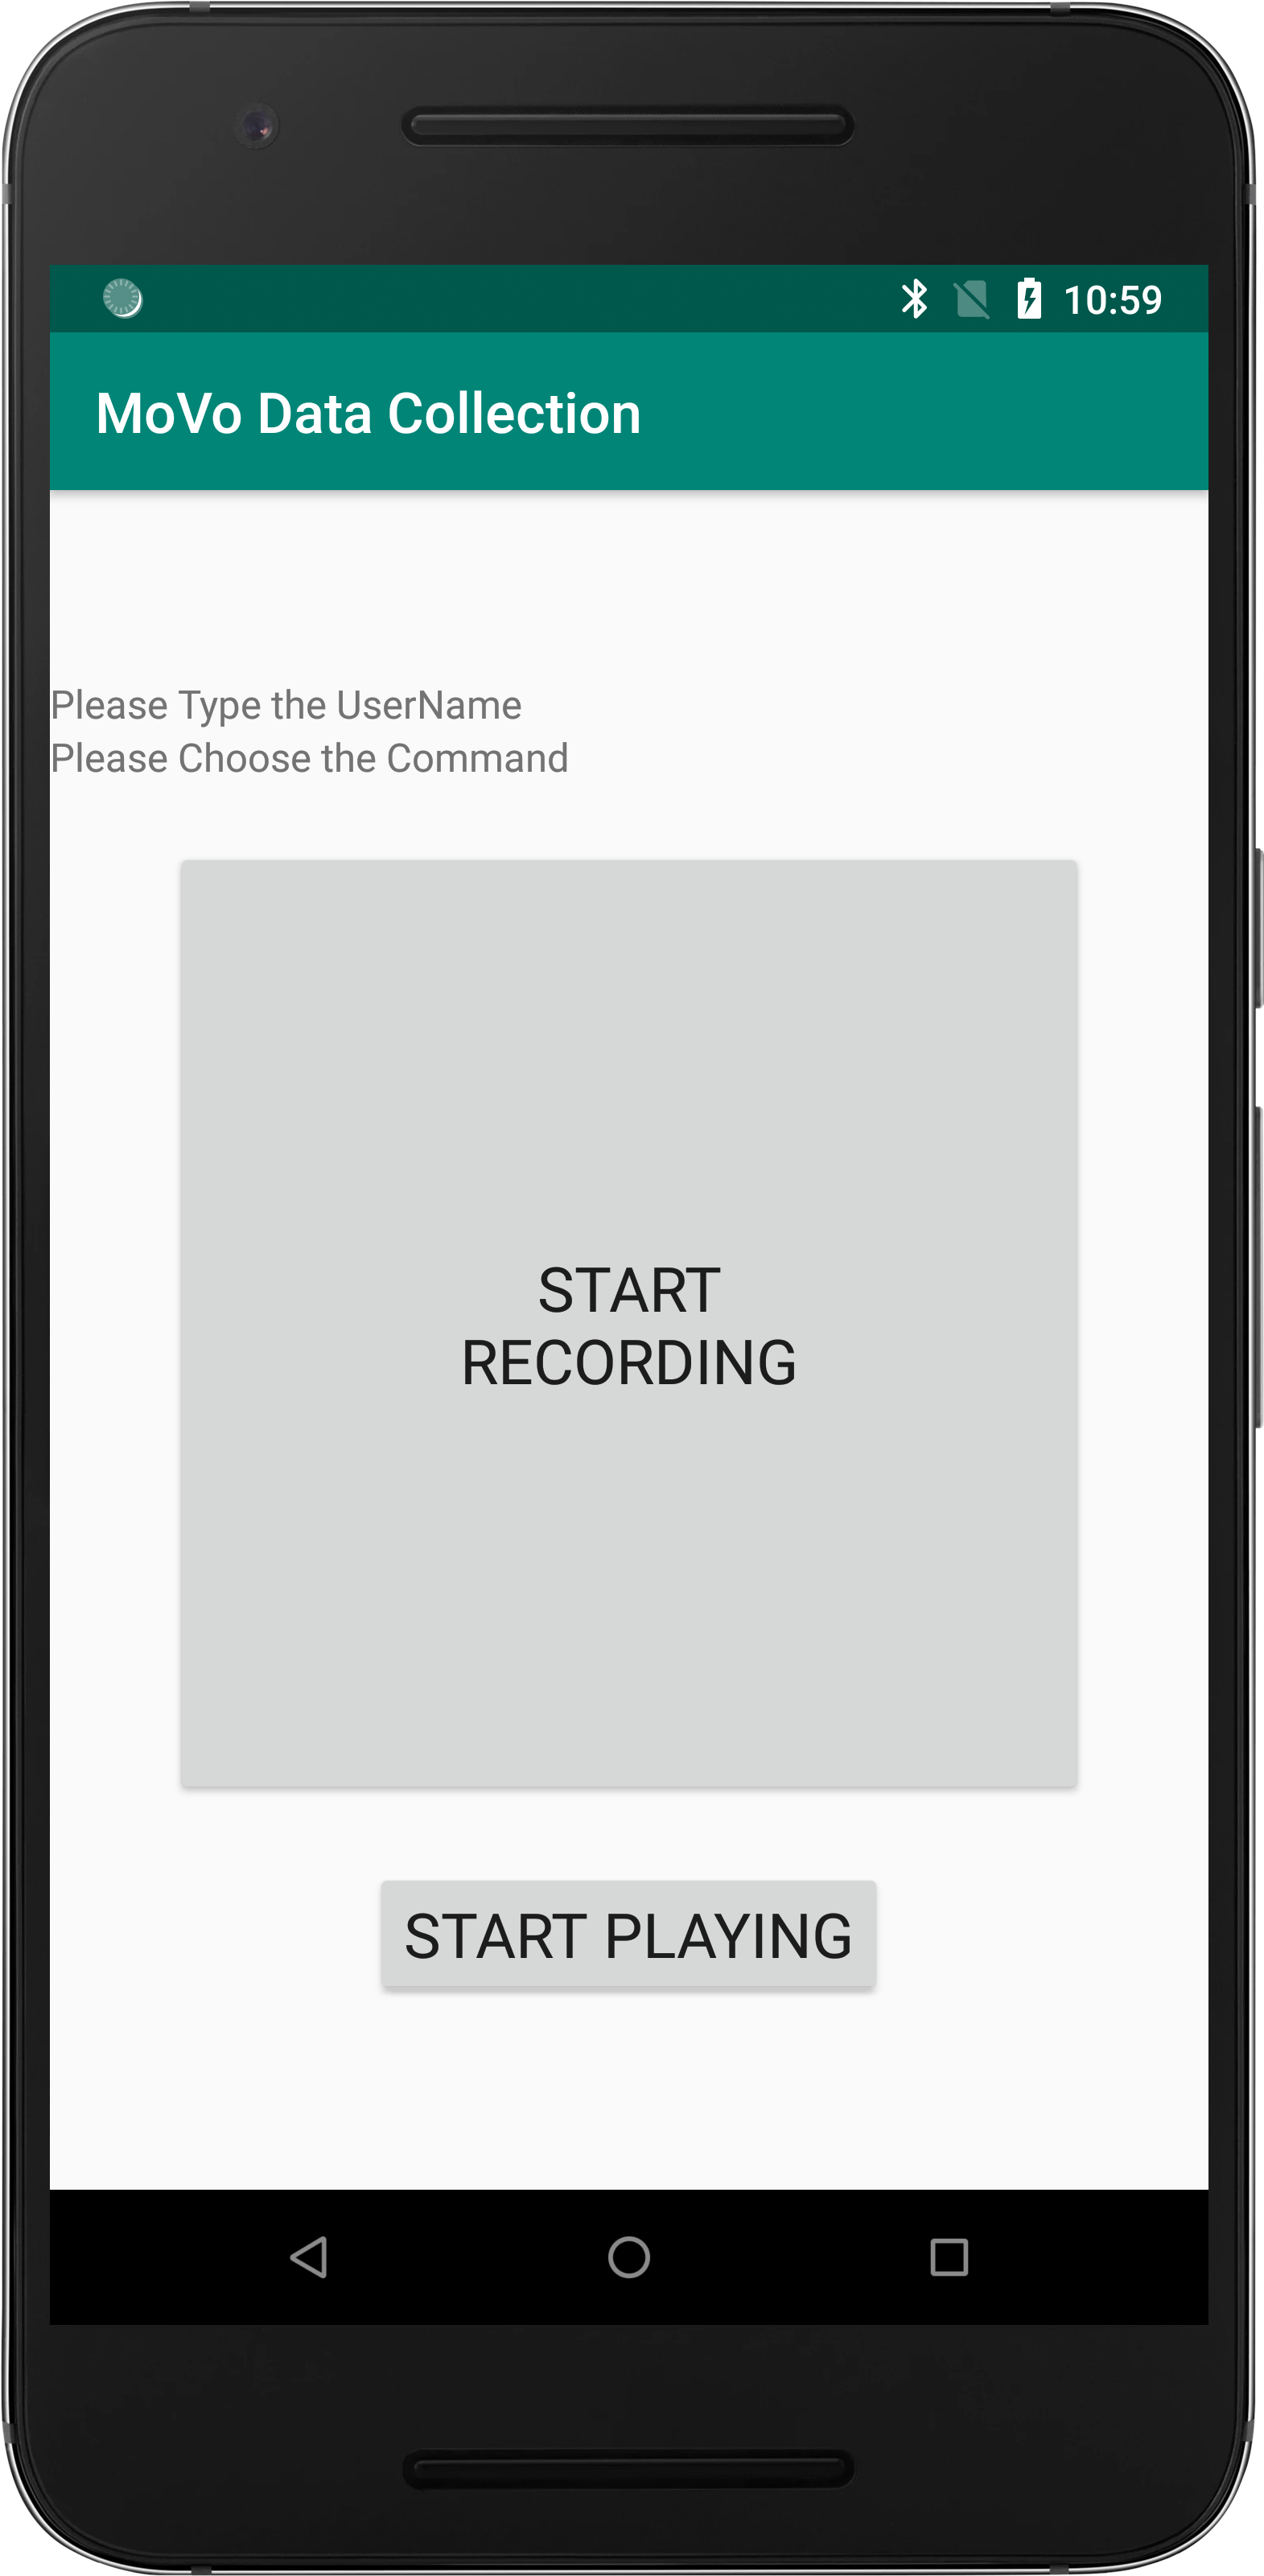
\includegraphics[height=.4\textheight]{MoVoData}
		\subcaption{{\mv} Data Collection}\label{fig:defendappa}
	\end{minipage}
	\qquad 
	\begin{minipage}{.6\linewidth}
		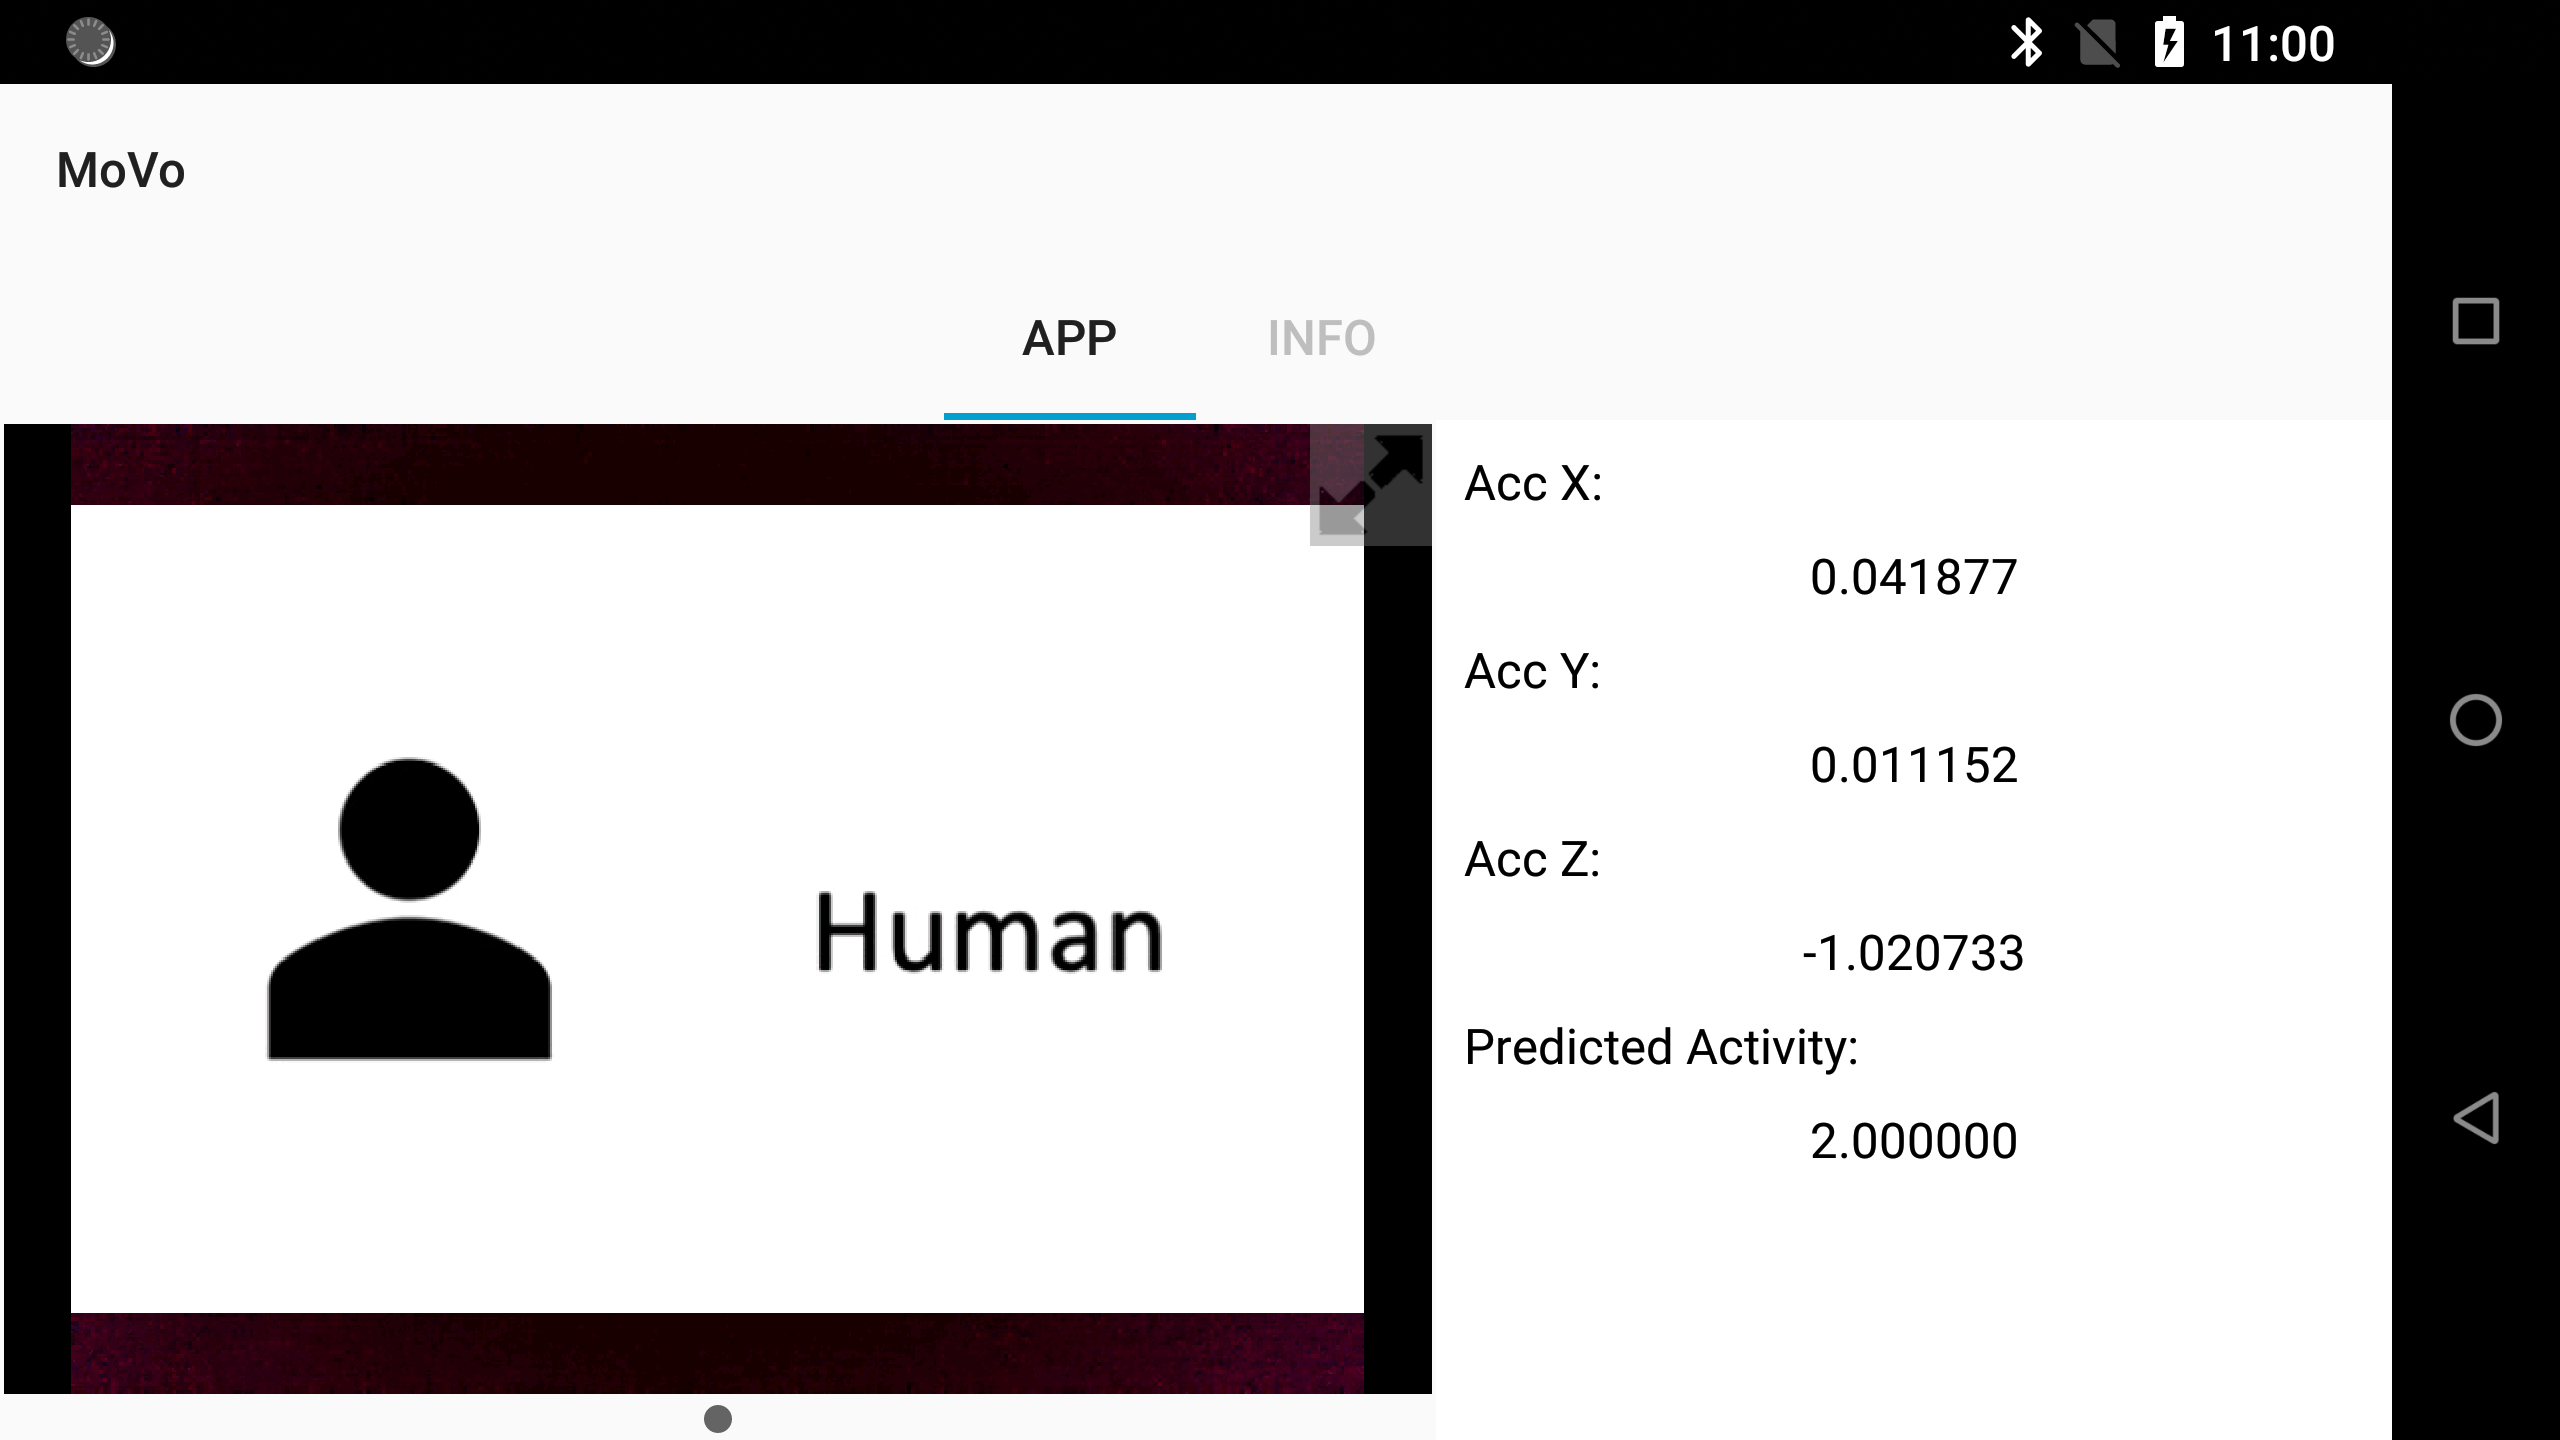
\includegraphics[width=\linewidth]{movohuman}
		\subcaption{Real Person Speaking}
		\vspace{.1in}
		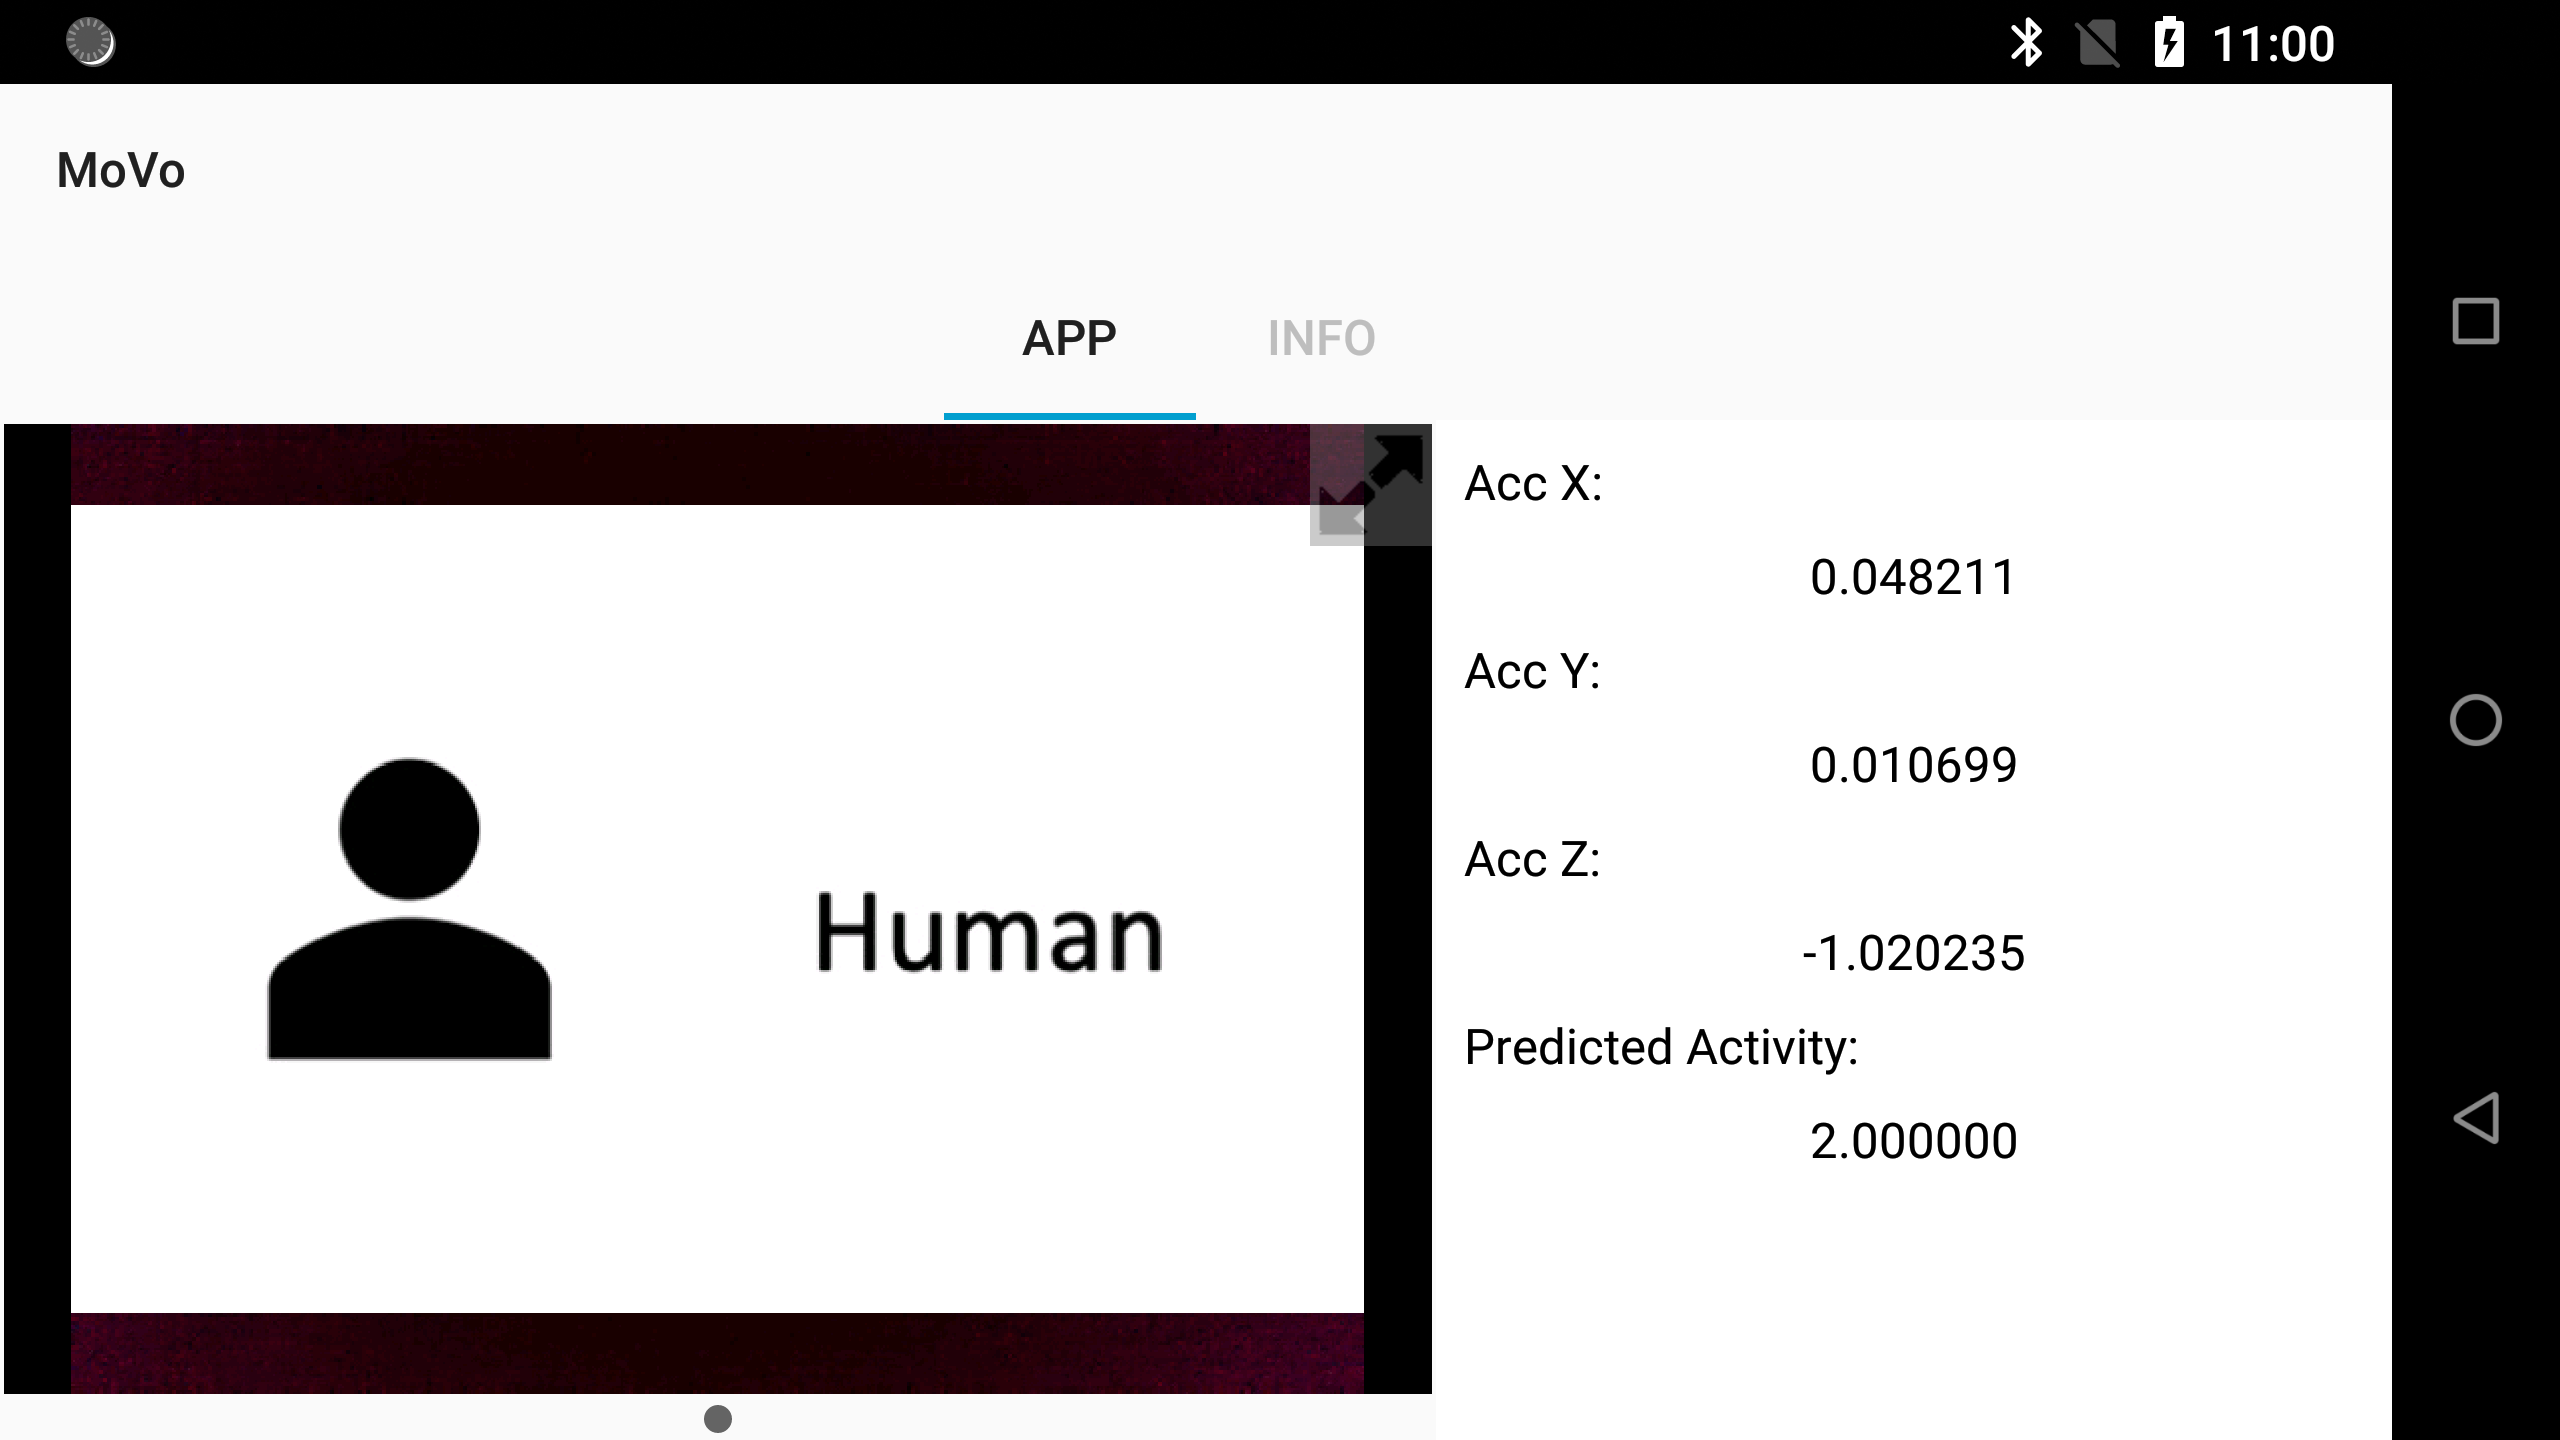
\includegraphics[width=\linewidth]{movodevice}
		\subcaption{Electronic Device Replaying Human Sounds}
		\vspace{.1in}
		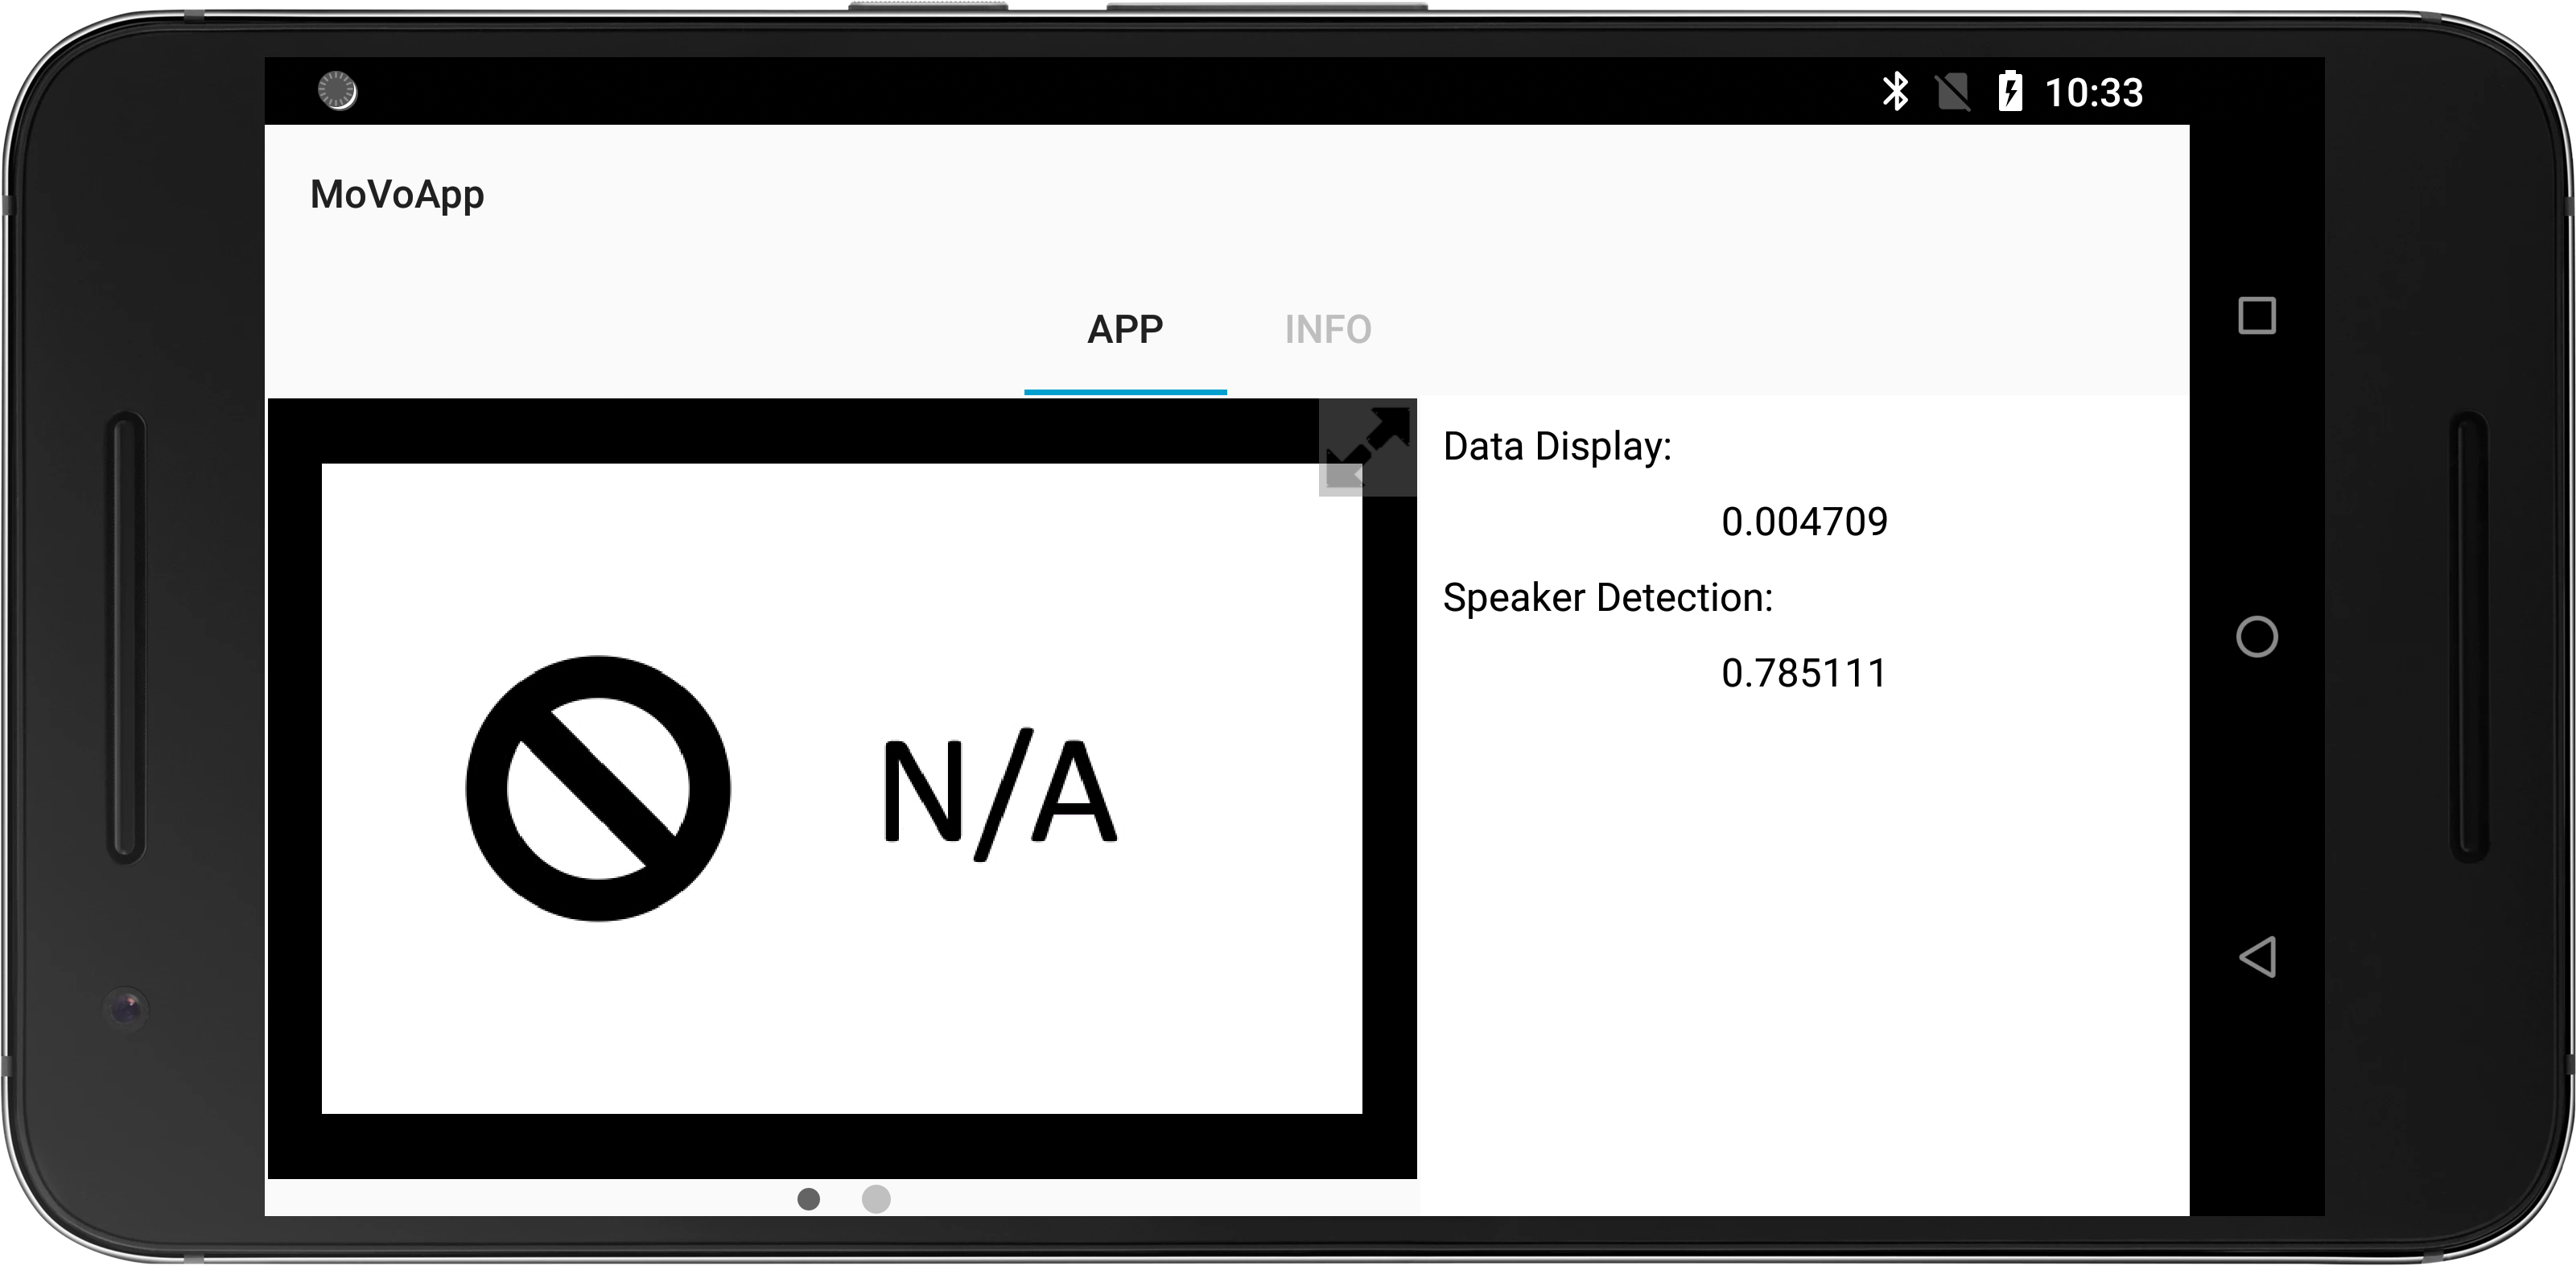
\includegraphics[width=\linewidth]{notapplicable}
		\subcaption{No Human Sounds}
	\end{minipage}
	\caption{Screenshots of the MoVo Data Collection App and MoVo Speaker Detection App}	
	\label{fig:defendapp}
\end{figure}

\textbf{Data Collection}. Our experiment involves 20 participants aged from 20 to 35. Among them, 13 are males and 7 are females; 15 are native English speaker and 5 uses English as a second language. For each user, we ask them to speak the following three hot-words: ``Ok Google'', ``Hi Siri'', and ``Alexa''. For each command, each user repeats it for 5 times. Therefore, we have 300 command samples in total. When we train our LSTM network, we are using the segmented motion data to train 10 different categories (`O', `K', `Goo', `Gle', `Hi', `Si', `Ri', `A', `Le', `Xa'). In this respect, we have 1000 sample sequences, where each sequence is about 100 samples long.


\begin{figure}[!h]
	\centering
	\begin{subfigure}[t]{0.45\textwidth}
		\centering
		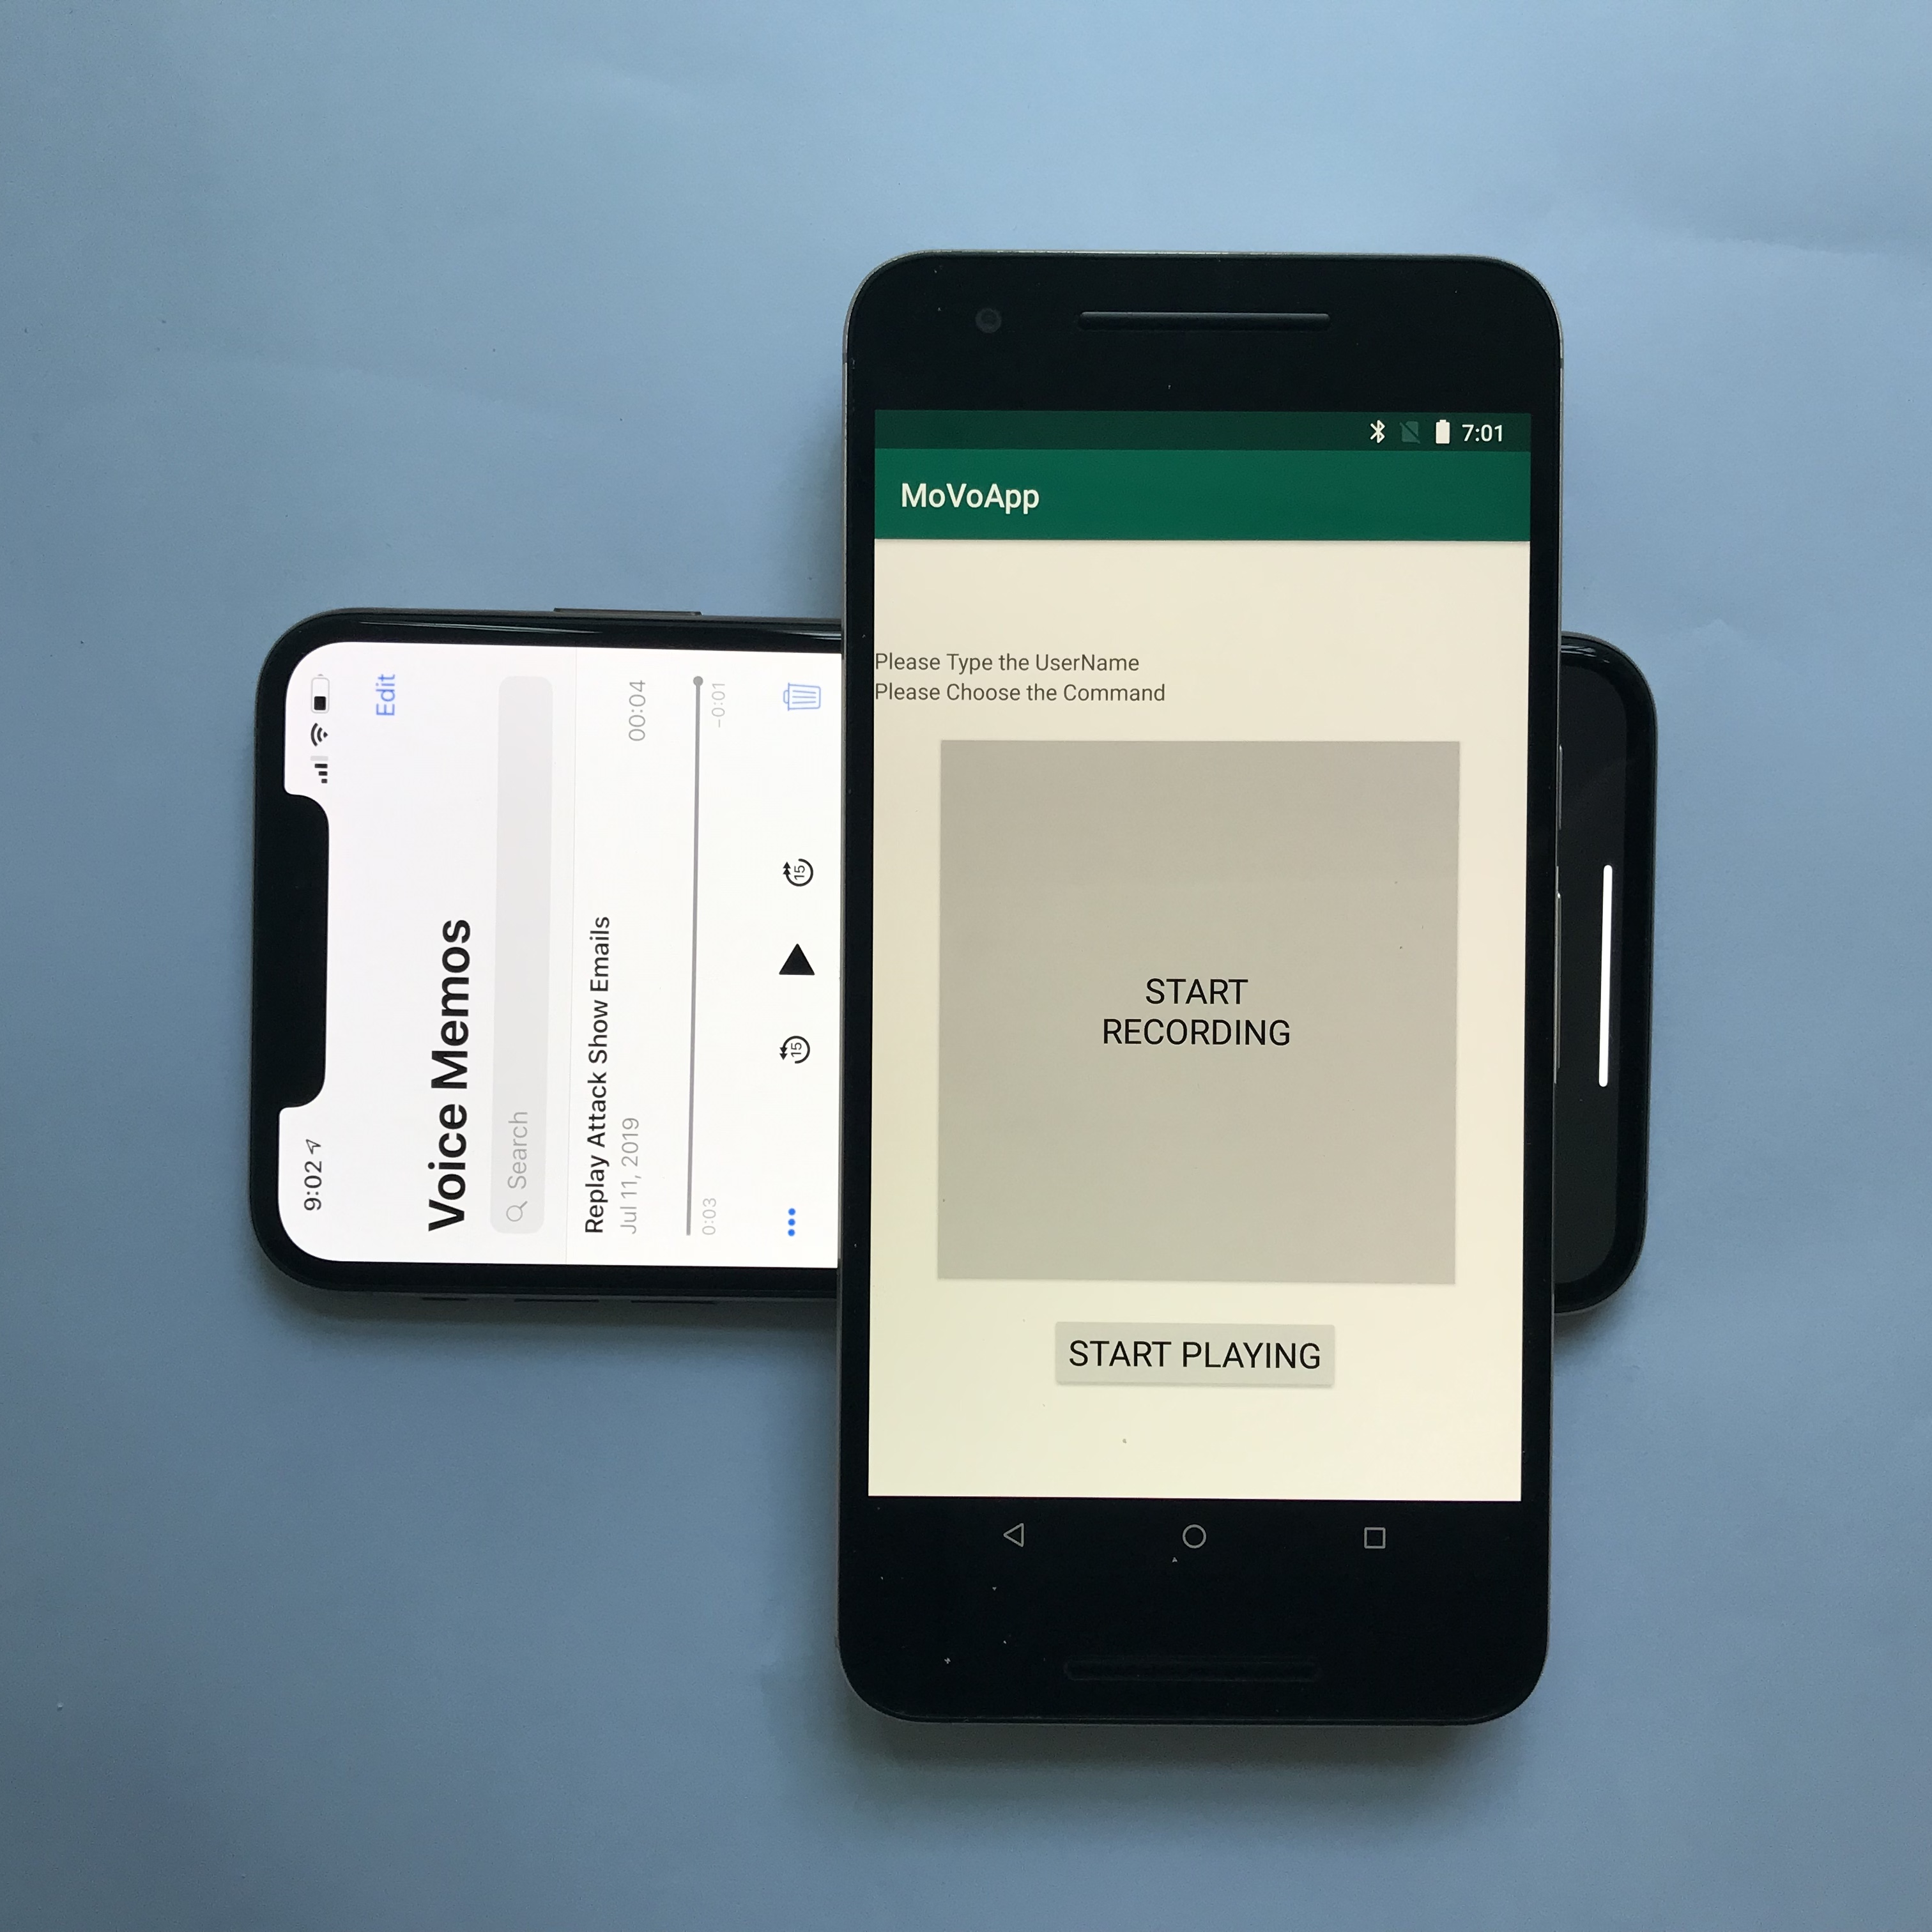
\includegraphics[height=\textwidth]{phone}
		\caption{Smartphone}
	\end{subfigure}%
	~ 
	\begin{subfigure}[t]{0.45\textwidth}
		\centering
		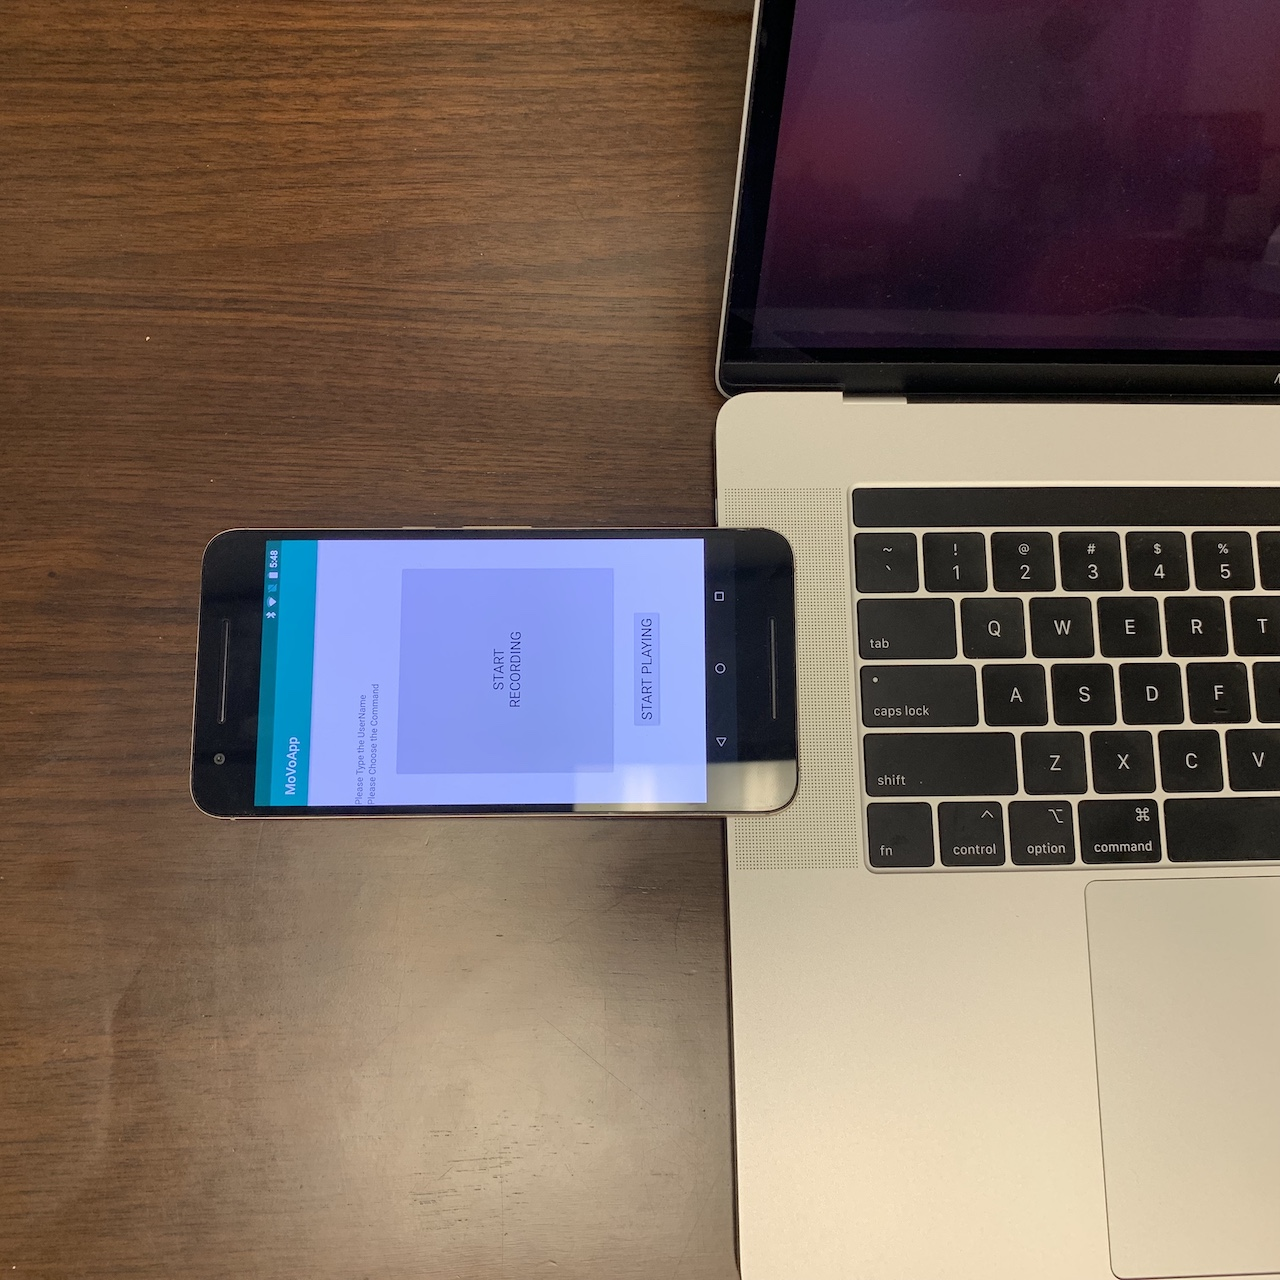
\includegraphics[height=\textwidth]{laptop}
		\caption{Laptop Speaker}
	\end{subfigure}
~ 
\begin{subfigure}[t]{0.45\textwidth}
	\centering
	\includegraphics[height=\textwidth]{desktop}
	\caption{Desktop Speaker}
\end{subfigure}
	~
	\begin{subfigure}[t]{0.45\textwidth}
	\centering
	\includegraphics[height=\textwidth]{mimic}
	\caption{Mimicry }
\end{subfigure}
	\caption{Attacker Settings}
	\label{fig:attacks}
\end{figure}





\textbf{Attacks}. As elaborated in Section~\ref{sec:attack}, we evaluate our system against three types of attack scenarios, simple playback attack, mimicry attack and sophisticated mimicry attack, where each scenario contains three kinds of attacks.  Since speech synthesis and voice conversion will generate speech signals similarly if use the same user's speech profile. Therefore, we only test the replay attack.

\begin{figure}[H]
	\centering
	\begin{minipage}{.35\linewidth}
		\includegraphics[width=\linewidth]{movoAttack}
		\vspace{.05in}
	\end{minipage}
	
	\centering
	\begin{tabular}{lr}
		\toprule
		Accuracy: 90.43\% & \hspace{-.55in} Error Rate: 9.57\% \\
		Precision: 90.72\% & \hspace{-.55in} True Positive Rate (Sensitivity/Recall): 90.52\% \\
		$F_1$ Score: 0.904 & \hspace{-.55in} True Negative Rate (Specificity): 95.19\% \\
		False Negative Rate: 9.48\%  & \hspace{-.55in} False Positive Rate: 4.81\% \\
		\bottomrule
	\end{tabular}
	\caption{Success rate of \shortname~on defending against various attacks. }
	\label{fig:defend}
\end{figure}


In simple playback attacks, the recordings of the legitimate user is replayed by either Logitech S120 2.0 Stereo Speakers, the built-in speakers of Apple Macbook Pro, and the built-in speaks of an Apple iPhone XS Max. Each of the 20 participants is considered as a legitimate user separately. For each participant, 5 attacks are conducted by the loudspeaker, 5 attacks are conducted by the laptop speaker, and 5 attacks are conducted by the iPhone speaker. All the three hot-words are tested. In total, there are 450 attacks. The attacking target is always Nexus 6P. The replay sound level is about 80dB, which is in consistent with the decibel level of normal human speech. 
The attacking device and the attacking target  are contacted, so that conductive vibrations are measured. 
In mimicry attacks, two smartphones are placed together and attached to the human throat. In sophisticated mimicry attacks, we consider 2 attackers: one male attacker to mimic the 7 male participants, and the other female attacker to mimic the 3 female participants. The attacker holds the phone tightly to his/her throat while replaying the target user's voice commands as in the simple playback attack cases. The sophisticated mimicry attack is repeated 10 times for each hot-word for each participant. Again, there are 450 such attacks. The final results are shown in Fig.~\ref{fig:defend}, \shortname~can defend replay attack with at least 90.43\% accuracy.

We have also implemented an application on Android to run {\uu} in real-time. As shown in Fig.~\ref{fig:defendapp}, the MoVoApp will decide among the following three cases: 1) a real human is speaking, 2) an electronic device is replaying human speeches, 3) no human sounds are made. Currently, this app only serves as an liveness detection app. We plan to add the user authentication features to this app  in future work. 
\begin{figure}[H]
	\centering
	\begin{minipage}{.35\linewidth}
		\includegraphics[width=\linewidth]{movoCommandbefore}
		\subcaption{Without Majority Voting}\label{fig:commadmata}
		\vspace{.05in}
	\end{minipage}
	\begin{minipage}{.35\linewidth}
		\includegraphics[width=\linewidth]{movoCommandafter}
		\subcaption{With Majority Voting}\label{fig:commadmatb}
		\vspace{.05in}
	\end{minipage}
	
	\centering
	\begin{tabular}{lr}
		\toprule
		Accuracy: 93.67\% & \hspace{-.55in} Error Rate: 6.33\% \\
		Precision: 93.67\% & \hspace{-.55in} True Positive Rate (Sensitivity/Recall): 93.71\% \\
		$F_1$ Score: 0.937 & \hspace{-.55in} True Negative Rate (Specificity): 96.84\% \\
		False Negative Rate: 6.29\%  & \hspace{-.55in} False Positive Rate: 3.16\% \\
		\bottomrule
	\end{tabular}
	\caption{Confusion Matrix of Matching Motion Data to Different Hot-Words. }
	\label{fig:commadmat}
\end{figure}


\textbf{Results}.
%
Besides defending against various attacks, \shortname~should accept legitimate users as in normal voice authentication systems. In other words, \shortname~should correctly classify a legitimate user's motion data to the hot-words he says. As shown in Fig.~\ref{fig:commadmat}, the overall accuracy of correct classification is 93.67\%.  
Note that we have two confusion matrices. Figure~\ref{fig:commadmata} is the original results provided by the machine learning network, while Figure~\ref{fig:commadmatb} is the result with majority voting procedure. There is a significant accuracy improvement with the presence of majority voting. Therefore, we only show the statistic evaluations of Figure~\ref{fig:commadmatb}. 


\begin{table}[t]
	\caption{Statistical Analysis of the User Classification Result}
	\label{tab:userTable}
	\centering
	\begin{tabular}{lr}
		\toprule
		Accuracy: 92.98\% & \hspace{-.55in} Error Rate: 7.02\% \\
		Precision: 93.33\% & \hspace{-.55in} True Positive Rate (Sensitivity/Recall): 94.58\% \\
		$F_1$ Score: 0.924 & \hspace{-.55in} True Negative Rate (Specificity): 99.64\% \\
		False Negative Rate: 5.42\%  & \hspace{-.55in} False Positive Rate: 0.36\% \\
		\bottomrule
	\end{tabular}
\end{table}



\begin{figure}[h]
	\centering
	\includegraphics[width=.5\linewidth]{movoTime}
	\caption{Robustness of {\shortname} over time.}
	\label{fig:time}
\end{figure}



The results for user authentication are shown in Fig.~\ref{fig:usermat} and Table.~\ref{tab:userTable}. Without majority voting, the accuracy of user authentication is only 54.48\%. With majority voting, the accuracy increases to 92.98\%. Note that this accuracy cannot beat existing speaker recognition systems based on audio files. Therefore, for better security, this result can serve as an extra channel of information. 

We also test the robustness of {\shortname} in Fig.~\ref{fig:time}. We test both the one-time trained model and the learning model which will use the accepted data as trained data for future authentication. Over 8 weeks, the learning model has more stable performance.






%We also evaluate the impact of feature dimensions on the classification accuracy. When we train the sequence-to-sequence LSTM network, we use all six dimensions of the motion data. In fact, different dimensions impact the classification result differently. As shown in Fig.~\ref{fig:axis}, accelerometer data are more useful in the classification than the gyroscope data. The more dimensions we use, the higher accuracy we can achieve. Among all single dimensions, the z direction of accelerometer is the best, which is the direction perpendicular to human throat surface. This is because the vibration on this direction is larger and easier to be caught by the accelerometer.
%
%\begin{figure}[h]
%	\centering
%%	\includegraphics[width=.6\linewidth]{axis}
%	\caption{Classification accuracy using different feature dimensions in the sequence input layer of our LSTM network.}
%	\label{fig:axis}
%\end{figure}







%\textbf{Discussion}. 
%Our \shortname~have some limitations. For example,  the number of evaluation participants and the size of hot-words dataset are relatively small. A larger dataset can be very useful to help evaluate the system though the technique contribution is limited. Another limitation is the overall classification accuracy. This shortcoming can be easily overcome by building a user-dependent classification model instead of the current user-independent one.  We have tested on the same dataset and found that the classification accuracy increases from 85.3\% to 93.7\% as shown in Fig.~\ref{fig:depenmat}. 

%\begin{figure}[H]
%	\centering
%	\includegraphics[width=.4\linewidth]{depenmat}
%	\caption{Confusion matrix of matching motion data to different hot-words when training the user-dependent LSTM model.}
%	\label{fig:depenmat}
%\end{figure}
%TODO more evaluation
%\begin{itemize}
%\item
%Evaluate different gender
%\item
%Evaluate user-dependent
%\item
%Evaluate Walking-Sitting-Running
%\item
%Evaluate syllable separation vs. process as a whole
%\item
%Evaluate high pass filter
%\item
%Evaluate majority voting
%\item
%compare with other algorithms (Spinx, SVM,...)
%\item
%Evaluate against different smartphones
%\item
%More person
%\end{itemize}


%Currently, we have implemented 4 traditional features (min, max, skewness, std. deviation)  and test the accuracy on 3 commands (‘Hi Siri’ and ‘Ok Google’). In total, we have 180 samples and each has a feature vector of length 32. By using the MATLAB classification app, we could achieve the maximum accuracy of 89%, which is achieved by the Quadratic Support Vector Machines.

%


\section{conclusion}

Self demodulation and acoustic attenuation can be used to build {\shortname}, a spoof-proof voice authentication system. When a user speaks with the smartphone placed on his throat, his voice not only influences the microphone readings, but also affects the accelerometer and gyroscopes. By adopting a sequence-to-sequence long short-term memory network, syllable separation, and majority voting, \shortname~can defend against 3 different types of attacks with 90.43\% defend rate and a 92.98\% acceptance rate for legitimate users.




\begin{landscape}
	\begin{figure}[h]
		\centering
		\begin{minipage}{.48\linewidth}
			\includegraphics[width=\linewidth]{movoUserBefore}
			\subcaption{Without Majority Voting}\label{fig:usermata}
			\vspace{.05in}
		\end{minipage}
		\begin{minipage}{.48\linewidth}
			\includegraphics[width=\linewidth]{movoUserAfter}
			\subcaption{With Majority Voting}\label{fig:usermatb}
			\vspace{.05in}
		\end{minipage}
		\caption{Confusion Matrix of Matching Motion Data to Different Users.}
		\label{fig:usermat}
	\end{figure}
\end{landscape}

